\documentclass[12pt,a4paper]{scrreprt}
\usepackage[latin1]{inputenc}
\usepackage[T1]{fontenc}
\usepackage{ngerman}
\RequirePackage[ngerman=ngerman-x-latest]{hyphsubst}
%\usepackage[ngerman]{babel}
\usepackage{amsmath}
\usepackage{amsfonts}
\usepackage{amssymb}
\usepackage{pgf}
\usepackage{listings}
\usepackage{url}
\usepackage[babel,german=quotes]{csquotes}
\usepackage[raggedright]{sidecap}
\usepackage{tabularx}
\usepackage[onehalfspacing]{setspace}
\usepackage{geometry}
\usepackage{color}
\usepackage{listings}
\usepackage{subfigure}
\usepackage{graphics}
\usepackage{wrapfig}
\usepackage{caption}
\usepackage{tabularx}
\usepackage[bottom,hang,multiple]{footmisc}

\newcolumntype{L}{>{\raggedright\arraybackslash}X}
\newcolumntype{Q}{>{\raggedright\arraybackslash}p{.13\linewidth}}

\captionsetup{format=plain,font=small,labelfont=bf}

\lstloadlanguages{bash,sh,Java,Ruby,Ant,XML}
\lstset{basicstyle=\footnotesize, escapechar={~}, stringstyle=\ttfamily, frameround=fttt, frame=trBL}

\geometry{a4paper, top=26mm, left=26mm, right=26mm, bottom=35mm, headsep=10mm, footskip=15mm}

\newcommand{\mycite}[1]{\enquote{\emph{#1}}}
\newcommand{\cd}{Continuous"=Delivery}
\newcommand{\ci}{Continuous"=Integration}
\newcommand{\devops}{DevOps}
\newcommand{\zb}{z.~B.}
\newcommand{\rc}{Release"=Candidate}
\newcommand{\dpipe}{Deployment"=Pipeline}
\newcommand{\comstage}{Commit"=Stage}
\newcommand{\acstage}{Acceptance"=Stage}
\newcommand{\uastage}{User"=Acceptance"=Stage}
\newcommand{\capstage}{Capacity"=Stage}
\newcommand{\prodenv}{Production}
\newcommand{\hf}{Humble und Farley}
\newcommand{\go}{\emph{Go}}
\newcommand{\dr}{\emph{Dreadnot}}
\newcommand{\dpl}{\emph{Deployinator}}
\newcommand{\ssp}{Self"=Service"=Portal}
\newcommand{\verskont}{Versionskontrollsystem}
%\newcommand{\comment}[1]{\vspace{1.5\baselineskip}\noindent\begin{addmargin}[3cm]{1.5cm}\begin{scriptsize}\textit{\emph{Kommentar:} #1 \vspace{1.5\baselineskip}}\end{scriptsize}\end{addmargin}}
\newcommand{\comment}[1]{}

\newcommand{\zitat}[1]{\enquote{\emph{#1}}}

\newcommand{\TODO}[1]{\framebox{\begin{minipage}{\linewidth}\begin{footnotesize}\texttt{\color{red}{TODO:\\#1}}\end{footnotesize}\end{minipage}}\\}

\newcommand{\quelle}[1]{\begin{flushright}{\small Quelle: #1 .}\end{flushright}}

\hyphenation{Dev-Ops}
\hyphenation{Con-tin-uo-us}
\hyphenation{De-live-ry}
\hyphenation{In-te-gra-tion}
\hyphenation{Vor-gehens-mo-dell}
\hyphenation{w�n-sch-ens-wert}
\hyphenation{Ver-sions-kon-troll-sys-tem}
\hyphenation{Frame-work}
\hyphenation{Dri-ven}
\hyphenation{De-vel-op-ment}
\hyphenation{De-ploy-ment}
\hyphenation{Man-age-ment}
\hyphenation{Feed-ba-ck}


\begin{document}

\begin{titlepage}

\noindent
\begin{minipage}{\linewidth}
\begin{minipage}{.5\linewidth}
\begin{flushleft}

\includegraphics[scale=.8]{Grafiken/FH_logo.jpg}
\end{flushleft}
\end{minipage}
\begin{minipage}{.5\linewidth}
\begin{flushright}
\includegraphics[scale=.8]{Grafiken/adesso_claim_4C.png} 
\end{flushright}
\end{minipage}
\end{minipage}

\vspace{6\baselineskip}

\begin{center}
%\maketitle

\begin{large}
\textbf{Master-Thesis}\\\vspace{2\baselineskip}
\end{large}

\begin{LARGE}
\begin{onehalfspace}
Evaluierung von ausgew�hlten Werkzeugen zur Realisierung von Continuous Delivery im Vergleich zur aktuellen Auslieferungspraxis von Software der adesso~AG
% Vergleich von Ans�tzen?
% Vergleich von Werkzeugen: Thoughtworks Go, Etsy Deployinator, Rackspace Dreadnot.
% Umsetzung von Continuous Delivery? (Gibt es wirklich ein Projekt)
% Softwareprojeke der adesso~AG: J2EE / Java-Web-Anwendungen / Bsp-Stack: Tomcat-Server, JSF 2.1, Oracle-DB (v. 11)
\end{onehalfspace}
\end{LARGE}

\vspace{2\baselineskip}

\begin{large}
\begin{tabular}{ll}
Verfasser: & Andr� G�rtner\\
 & F�hrhofstra�e 28a\\
 & 18439 Stralsund\\
Erstkorrektor: & Prof.~Dr.~rer.~nat. Gerold Blakowski\\
Zweitkorrektor: & Dipl.~Ing.(FH) Dieter Gaikowski
\end{tabular}
\end{large}

\end{center}

\vfill

\begin{tabular}{ll}
Datum & \today \\
Kontakt E-Mail: & swangaer@gmail.com\\
\end{tabular}

\end{titlepage}

\renewcommand{\thepage}{\Roman{page}}
\setcounter{page}{1}

\tableofcontents

\listoffigures

\lstlistoflistings

\chapter*{Abk�rzungsverzeichnis}

\begin{tabularx}{\linewidth}{LL|LL}
BGB & B�rgerliches Gesetzbuch & IaaS & Infrastructure as a Service\\
\end{tabularx}

\newpage
\renewcommand{\thepage}{}

\part{Master-Thesis}

\renewcommand{\thepage}{\arabic{page}}
\setcounter{page}{1}

\chapter{Einleitung und Zielstellung}

Diese Arbeit setzt sich mit dem Themenkomplex von \cd\ auseinander. Wolf Schlegel formulierte die Zielstellung von \cd\ in einem Artikel folgenderma�en: \zitat{Software ist erst dann fertig, wenn sie produktiv eingesetzt wird.}\footnote{Vgl. \cite{schlegel}} Damit wird der Schritt, die Anwendung in die Produktivumgebung zu heben, in einen besonderen Fokus gesetzt.

% Was ist CD

In den sp�ten 90er Jahren arbeitete Kent Beck f�r ein Versicherungsunternehmen in der Schweiz, bei der jede Nacht in das Produktivsystem ausgeliefert wurde. Dieses Verfahren war f�r den Versicherer von Vorteil, da fertige und produktiv einsetzbare Software nicht erst auf das n�chste Release in drei Monaten warten musste, wie in anderen Projekten �blich, sondern schon am n�chsten Tag gewinnbringend eingesetzt werden konnte.\footnote{Vgl. Vorwort von Martin Fowler in \cite[S. xxi]{CD}}

Das erste der 2001 verfassten 12 Prinzipien aus dem Manifest f�r Agile Softwareentwicklung, nachfolgend kurz \emph{Agiles Manifest} genannt, priorisiert eine fr�he und kontinuierliche Auslieferung von wertvoller Software.\footnote{Vgl. \cite{manifesto}} Mit \cd\ wird ein Prinzip des \emph{Agilen Manifests} umgesetzt. Daraus kann abgeleitet werden, dass aus der Sicht des Kunden, durch jeden Entwicklungsschritt der Wert der Software erh�ht wird und der daraus resultierende Nutzen fr�hestm�glich auch produktiv eingesetzt werden sollte. Ein Ziel, das Kent Beck in dem zuvor genannten Versicherungsprojekt bereits verwirklichen konnte.

In dem agilen Vorgehensmodell Scrum wird der Prozess der Softwareentwicklung in Iterationen mit einer Dauer von 2 bis 4 Wochen unterteilt. Jede Iteration soll eine Version der Software liefern, die mehr f�r den Kunden n�tzliche Funktionalit�ten bereitstellt, als die Version der vorhergehenden Iteration.\footnote{Vgl. \cite{scrum_wirdemann}}

Anforderungen erf�llt, ist eine Inbetriebnahme dieser Version vom Kunden durchaus w�nschenswert. Bei einem Kunden-Lieferanten-Verh�ltnis kann dem Kunden dann die M�glichkeit einger�umt werden, die aktuelle Version zu testen, abzunehmen und die so bereitgestellten Funktionalit�ten schon produktiv einzusetzen. Die Entwicklung ist zu diesem Zeitpunkt noch nicht abgeschlossen und weitere geplante Funktionalit�ten k�nnen folgen. Nachfolgende Entwicklungsschritte erfordern dann aber wiederum weitere Abnahmetests und Inbetriebnahmen der neuen Version. Bis zum Ende der Projektlaufzeit k�nnte diese mehrere Wiederholungen des Abnahmeprozesses nach sich ziehen. Bei der Forderung eine Software kontinuierlich in kleinen Schritten auszuliefern, wird die dahinterstehende Komplexit�t nicht unmittelbar ersichtlich, die sich aus der Bereitstellung einer Software in der spezifizierten Produktivumgebung verbirgt. 

Nach Steinweg umfasst die Einf�hrung einer Software die Phasen der Werkabnahme, des Pilotbetriebs, der offiziellen Abnahme, dem Rollout, dem Training der Anwender und dem Going-Live.\footnote{Vgl. \cite[S. 172 ff]{steinweg04}} Bei der Werkabnahme ist der Besteller nach �~640 Absatz~1 Satz~1 BGB verpflichtet, das vertragsm��ige Werk abzunehmen. Dieser Schritt ist notwendig, damit M�ngel beim Hersteller des Werkes fristgerecht angezeigt werden k�nnen und der Kunde seine in �~634 Nr.~1 bis~4 BGB aufgef�hrten Rechte auf die Nacherf�llung, den Ersatz f�r erforderliche Aufwendungen, den Vertragsr�cktritt, die Minderung oder den Schadensersatz wahrnehmen kann. Damit sind aber auf Kundenseite auch nicht zu untersch�tzende Aufw�nde f�r die Abnahme der Software in den geregelten Betrieb einzuplanen.

\cd\ verspricht durch die Automatisierung und eine klare Prozessgestaltung die Komplexit�t des Liefervorgangs zu reduzieren. Es soll die Basis eines schnellen und zuverl�ssigen Software-Lieferprozess bereitstellen.\footnote{Vgl. \cite{schlegel}} Soll f�r ein Projekt ein teil- bzw. vollautomatisierter Prozess umgesetzt werden, m�ssen zuvor nicht nur eine Reihe technischer Probleme, sondern auch vielmehr vertragliche und organisatorische Implikationen auf einen automatisierten Lieferprozess betrachtet werden. \cd\ wird aber erst durch Technologie erm�glicht.

\cd\ steht in einem engen Zusammenhang mit der \devops -Bewegung. \devops\ fordert die engere Zusammenarbeit von Softwareentwicklern und IT-Betrieb als die Weiterentwicklung der agilen Vorgehensmodelle. Durch die konsequente Verwirklichung, neue Funktionalit�ten dem Kunden schnellstm�glich bereitstellen zu k�nnen, sind neue Strukturen in der Organisation von Entwicklungsteams notwendig. \cd\ ist in diesem Zusammenhang die technologische Verwirklichung von \devops , da es hilft, Kommunikationsbarrieren zwischen den Teilbereichen Betrieb und Entwicklung abzubauen. \devops\ selbst fokussiert keinen spezifischen Technologie-Stack. Die Ideen zu \devops\ und \cd\ stammen aber von Personen, die besonders aktiv im Umfeld von Web~2.0-Anwendungen und Cloud-Computing sind. 

Die Anforderung, eine neue Funktionalit�t den Anwendern m�glichst vor der Konkurrenz bereitstellen zu k�nnen, ist in diesem Umfeld besonders hoch. Der Prozess, eine neue Funktionalit�t in die Produktionsumgebung auszuliefern, muss deshalb schnell und ohne zus�tzlichen Aufwand ablaufen k�nnen. Beim Ausliefern einer neuen Softwareversion darf aber nicht das Risiko des Scheiterns des Prozesses missachtet werden. Ein Webshop mit vielen tausend aktiven Nutzern, der nach einem Update pl�tzlich nicht mehr verf�gbar ist oder schwere Fehler \zb\ bei der Kalkulation des Preises macht, kann einen hohen wirtschaftlichen Verlust verursachen. Automatisierte Tests und das st�ckweise Aktualisieren der Anwendung sowie ein sofort verf�gbares Roll-Back Konzept sind daher auch Komponenten von \cd . 

In seinem Blog-Eintrag aus dem Jahr 2009 ging Timothy Fitz auf das Thema \cd\ ein. In diesem schrieb er, dass l�ngere Releasezyklen in Projekten problematisch sein. Er sah, dass auch kleinere Fehler, die erst in der Produktionsumgebung durch hervortreten, \zb\ durch eine andere Konfiguration oder andere Systembedingungen, sehr schwierig sind, zu beheben. Er beschrieb, wie durch ein einfaches Refactoring einer Anwendung kleinere Fehler in die Quellcode-Basis gebracht wurden. Der Fehler trat auf, als die Anwendung zwei Wochen sp�ter in Produktion ausgeliefert wurde. Da es ein Konfigurationsfehler war, der das Produktivsystem betraf, konnte der Fehler durch die Qualit�tssicherung nicht entdeckt werden. Erst nach mehrst�ndiger intensiver Inspektion konnte der Fehler entdeckt werden und Anwendung wieder produktiv gehen. Die Erinnerung an die durchgef�hrten �nderungen waren nur noch ungenau vorhanden, da die �nderung schon zwei Wochen her war. Fitz empfahl nach diesem Vorfall t�glich in die Produktionsumgebung auszuliefern. Er ging davon aus, dass dieser Fehler auch nicht durch die Steigerung von automatisierten Tests zu vermeiden gewesen w�re. Der Prozess selbst war das Problem. W�re die Anwendung direkt nach dem Refactoring und dem Durchlauf der Tests in die Produktivumgebung ausgeliefert worden, h�tte die Auswirkung schneller mit der durchgef�hrten �nderung in Verbindung gebracht werden k�nnen.\footnote{Vgl.  \cite{fitz_cd}}

In den nachfolgenden Kommentaren zu seinem Vorschlag fanden sich viele Aussagen wie \mycite{unrealistisch}, \mycite{funktioniert nicht}, \mycite{geht nur mit kleineren Anwendungen}, \mycite{nette Theorie, aber kann nicht klappen}. Ein weiterer Verfasser eines Kommentars hatte auf die Anforderungen eines komplexen Finanztransaktionssystem hingewiesen, in dem alle Transaktionen einer fehlerhaften Version m�glicherweise wieder r�ckg�ngig gemacht werden m�ssten. F�r den Verfasser kann ein direktes Ausliefern der Anwendung in die Produktivumgebung nur f�r kleinere Anwendungen mit geringem Funktionsumfang m�glich sein. Die Nutzung dieses Konzeptes f�r Testumgebungen h�lt er jedoch f�r lohnenswert.\footnote{Vgl.  \cite{fitz_cd}}

%Beispielsweise entstanden die Cloud-Dienste von Amazon aus der internen Anforderung den Entwicklern einer Shopkomponente die ben�tigte Infrastrukturen zum Testen und Ausf�hren der Komponente �ber ein Selbstbedienungsportal beziehen zu k�nnen. Hierf�r bildete Amazon Teams die alle F�higkeiten, die zur Entwicklung und zum Betrieb der Anwendung notwendig sind, auf sicher vereint.

Auf Ebene der Betriebssysteme ist es m�glich wiederkehrende Vorg�nge, wie Programmaufrufe, Softwareinstallationen oder Dateibewegungen, in Shell-Skripten zu verfassen und vom System jederzeit wieder ausf�hren zu lassen. So k�nnte das Kompilieren des Quellcodes oder die Bereitstellung einer Software auf einem Testsystem in einem derartigen Kleinstprogramm beschrieben werden. �ber die Systemkonsole lie�e sich dieses jederzeit auf die gleiche Art und Weise ausf�hren. Eine Teilautomatisierung des existierenden Auslieferungsprozess w�rde so schon realisiert werden k�nnen. Dieser w�rde allerdings nur aus einer losen Sammlung von Skripten bestehen, die auf eine konsistente Aufrufreihenfolge angewiesen sind. Wenn die Prozesse der Softwareerstellung, des Tests und der Lieferung auf entfernten Systemen durchgef�hrt werden, ist die Durchf�hrung m�glicherweise nur auf einen bestimmten Personenkreis beschr�nkt, welcher Zugriffsrechte auf die entfernten Systeme besitzt.

Der Problematik, den Lieferprozess von jedem Mitglied des Entwicklungsteam durchf�hren lassen zu k�nnen ohne aber die Systemrechte an alle zu verteilen, standen auch eine Reihe von Projekten im Bereich der Webanwendungen gegen�ber, die in eigene L�sungen m�ndeten. Einige dieser L�sungen, wie \dpl\ und \dr\ wurden unter eine quelloffene Lizenz gestellt und einer breiten �ffentlichkeit zur Nutzung und Weiterentwicklung zug�nglich gemacht.\footnote{Vgl. \cite{codeascraft}} Daneben haben auch Hersteller propriet�rer Software den Bedarf an derartigen L�sungen entdeckt und bieten Systeme, wie \go\ von Thoughtworks, unter dem Schlagwort \cd\ an.\footnote{Vgl. \cite{go_product}}

%Dieser letzte Schritt stellt sich h�ufig als ein sehr schwieriger dar und ist nicht selten mit hohen Aufw�nden bei der Planung und Durchf�hrung verbunden. Aus diesem Grund wird in Softwareprojekten gew�hnlich nur eine �berschaubare Anzahl von Terminen f�r eine Auslieferung vereinbart, um den damit verbundenen Aufwand m�glichst gering zu halten. \cd\ bietet hier einen anderen Ansatz an. Der Prozess, beginnend mit dem \emph{Commit} von Quellcode in ein Repository bis hin zur Auslieferung der fertigen Software auf die Produktionsumgebung, wird mit Hilfe von Werkzeugen und organisatorischen Ma�nahmen weitgehend automatisiert gestaltet. Eine Bedingung von \cd\ ist, nur getestete und fehlerfreie Software auf das Zielsystem auszuliefern. \cd\ versucht durch Automatisierung die Basis f�r einen schnellen und zuverl�ssigen Software-Lieferprozess herzustellen.\footnote{Vgl. \cite{schlegel}}

% Management der Softwareentwicklung S. 174 ff -> Roll Out, Teilabnahme eines Werkes.
% Ziel:

Die adesso~AG, nachfolgend adesso genannt, ist ein unabh�ngiger IT-Dienstleister, der mit Beratung und Softwareentwicklung die Kerngesch�ftsprozesse seiner Kunden optimiert.\footnote{Vgl. \cite{ad_profil}} adesso besitzt dabei, neben anderen Technologien, eine Kompetenz im Java-Technologiespektrum. Dies umfasst auch besonders das Komponentenmodell der Java Enterprise Edition, kruz JEE. Auf dieser Basis verwirklicht adesso regelm��ig Projekte.\footnote{Vgl. \cite{ad_kompetenz_jee}}

F�r die Realisierung von neuen Softwareprojekten hat adesso ein eigenes agiles Vorgehensmodell, \emph{adVANTAGE}, entwickelt. \emph{adVANTAGE} soll die Entwicklung auf Basis eines grob kalkulierten Budgets erm�glichen. Anforderungen werden hierbei, �hnlich dem Vorgehen in Scrum, priorisiert und f�r Sprints ausgew�hlt und entwickelt. Bei der Auswahl stehen die f�r das Gesch�ft kritischen Anforderungen im Vordergrund, die f�r einen fr�hestm�glichen Start der Anwendung notwendig sind.\footnote{Vgl. \cite{ad_advantage}}

Hieraus ergibt sich f�r adesso ein Interesse am automatisierten Auslieferungsprozess und \cd . Im Unternehmen werden deshalb verschiedene Aktivit�ten rund um das Thema vorangetrieben. Dabei hat adesso drei Werkzeuge identifiziert, die einen Fortschritt f�r den derzeitigen Auslieferungsprozess bedeuten k�nnten. Folgende Werkzeuge sind zu untersuchen: 

\begin{itemize}
\item \go\ von Thoughtworks Studios\footnote{Informationen zu \go\ unter \\\url{http://www.thoughtworks-studios.com/go-agile-release-management}},
\item \dpl\ von Etsy\footnote{Informationen zu \dpl\ unter \url{https://github.com/etsy/deployinator}} und
\item \dr\ von Rackspace\footnote{Informationen zu \dr\ unter \url{https://github.com/racker/dreadnot/}}.
\end{itemize}

Der genaue Funktionsumfang der Werkzeuge ist nicht bekannt. Bekannt ist nur, dass diese in Verbindung mit \cd\ stehen. adesso m�chte aus diesem Grund einen �berblick �ber die Funktionalit�ten und Ans�tze dieser Werkzeuge gewinnen. Ziel dieser Arbeit soll deshalb die Evaluierung dieser sein. Dabei soll gepr�ft werden, ob eines der untersuchten Werkzeuge geeignet ist, um den derzeitigen Auslieferungsprozess sinnvoll zu erg�nzen. Aus diesem Grund m�ssen nicht nur die angef�hrten Werkzeuge untersucht, sondern auch der bestehende Auslieferungsprozess betrachtet werden. Einf�hrend besch�ftigt sich diese Arbeit mit der Kernfrage von \cd\ und beschreibt die entsprechenden Konzepte, die zum Verst�ndnis der Werkzeuge notwendig sind.

% Die technologische Kompetenz von adesso und den beschriebenen Vorteilen von CD f�hrt zum Interesse, CD in Software-Projekten den Kunden von adesso anbieten zu k�nnen.

% Drei Werkzeuge stechen durch ihren Beschreibungen als Werkzeuge f�r CD heraus. Es soll untersucht werden, ob diese Werkzeuge sich f�r einen Einsatz bei adesso eignen und welche Ans�tze diese dabei verfolgen. Dem gegen�ber steht die dezeitige Auslieferungspraxis von adesso. Um erkennen zu k�nnen, welche Werkzeuge sind gegebenenfalls eignen, muss der aktuelle Ausliefreungsprozess und die dabei verwendeten Werkzeuge n�her untersucht werden.

% Das Ergebnis der Arbeit ist eine Gegen�berstellung dre Ans�tze und Funktiosweisen von drei, von adesso als interessat eingestuften, Werkzeugen f�r CD. Der Vergleich mit der derzeitigen Auslieferungspraxis f�hrt m�glicherweise zu einer Werkzeugempfehlung, einer Verfahrensempfehlung oder zu einer Best�t�tigung des derzeitigen Vorgehens.

\comment{In der Einleitung wird die Motivation f�r das Thema aufgegriffen und erkl�rt warum dieses wichtig ist. Zudem wird der Bezug zu adesso gesetzt und die Perspektive erl�utert, die sich f�r adesso aus dem Thema ergibt.}

\comment{Welche Projekte werden bei adesso typischer Weise umgesetzt?}

\comment{Woher kommt \cd\ und was f�r Vorz�ge werden versprochen? Hier wird auf die Herkunft eingegangen und der Bezug zum Agilen Minifest gesetzt. \cd\ wird als ein Betrag zu DevOps gesehen und verspricht unter anderem einen qualitativen Softwarelieferprozess. Dies ist wichtig, um zu verstehen, was \cd\ erreichen will und gegen was die zu untersuchenden Werkzeuge zu pr�fen sind.}

\chapter{Entstehung und Konzepte von \cd}\label{konzepte_cd}

Um die Funktionalit�ten der zu untersuchenden Werkzeuge verstehen zu k�nnen, ist eine Betrachtung der Konzepte \cd\ notwendig. Dieser Abschnitt behandelt eingehend die Problemstellung von \cd , denen mit den hier vorgestellten Konzepten begegnet werden soll. Hinter den Ideen von \cd\ steht die \devops -Bewegung. Aus \devops\ leiten sich technische und organisatorische Implikationen wie \zb\ die \emph{Definition of Done}, der \rc , die Prozessautomatisierung und das Fast"=Feedback an das Entwicklungsteam ab. Wesentliche Bef�rderer dieses Themenkomplexes sind Jez Humble und David Farley, die in ihrem Buch \cd\ und die \dpipe\ zusammenh�ngend darstellen und L�sungsstrategien f�r technische Fragestellungen anbieten.\footnote{Vgl. \cite{CD}} \cd\ ber�hrt durch das automatisierte Auslieferungsverfahren auch die Domaine der ITIL Service Transitions gerade im Bereich von Service- und Release"=Management. Am Ende des Abschnitts wird mit einem Exkurs auf die gegenseitigen Implikationen von \cd\ und ITIL eingegangen.

\section{Die \devops -Bewegung}

%\comment{\cd\ ist ein Thema aus der DevOps-Bewegung. Das Zusammenwachsen von Entwicklung und Betrieb kann z.B. durch \cd\ verbessert bzw. sogar erst erm�glicht werden. Das soll hier beschrieben und gepr�ft werden. Ein \dpipe\ stellt im weiten Sinne einen Eingriff des Entwicklers in den klassischen Aufgabenbereich des IT-Betriebes ein. Wird das bei der umgesetzten Pipeline der Fall sein oder w�chst IT-Betrieb und Entwicklung nicht n�her zusammen?}

In der belgischen Stadt Genth fand unter dem Titel \devops -Days im Jahr 2009 eine Konferenz zu den Themen Build\footnote{Build bezeichnet den das Kompilieren und Paketieren von Quellcode.}, Softwaretest und Deployment\footnote{Deployment bezeichnet das Ausliefern von Softwarepaketen in eine Ausf�hrungsumgebung. Dies kann \zb\ eine Webanwendung sein, die von einem Webserver ausgef�hrt wird} statt.\footnote{Vgl. \cite{cd_devops_1}} Die Seite \url{www.DevOps.com} begr��t seine Besucher mit dem Slogan \mycite{Helping finish what Agile development started}\footnote{\cite{devopsdays.org2012}}. Dieser Slogan beschreibt das eigene Verst�ndnis der \devops -Bewegung. Chris Read schreibt in einem Gastbeitrag �ber \devops\ wie folgt: \mycite{At its heart it is the integration of Agile principles into Operations practices}. Dies erm�glichte nach seiner Ansicht die Clound- und Web-2.0"=Giganten.\footnote{Vgl. \cite{cd_devops_stateofnation}} \devops\ versucht im Kern die Kommunikation zwischen Systemadministratoren und den Entwicklern der Systeme zu verbessern. Die agilen Praktiken, wie sie zwischen Entwicklern und ihren Kunden schon fl�chendeckend betrieben werden, sollen auch zwischen IT"=Betrieb und Softwareentwicklern implementiert werden. Auch \hf\ sind in ihrem Buch der Ansicht, dass agile Techniken zum Managen von Infrastrukturen sehr gut geeignet sind.\footnote{Vgl. \cite[S. 279]{CD}}

\begin{wrapfigure}{r}{0.4\textwidth}
\centering
\fbox{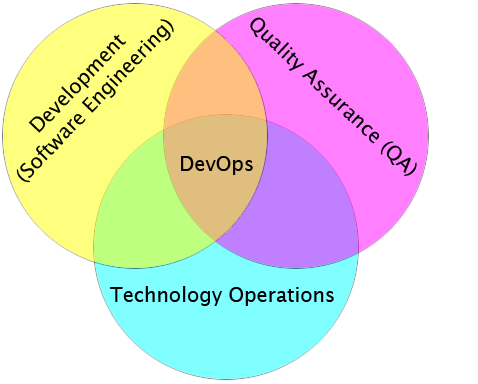
\includegraphics[width=\linewidth]{Grafiken/devops.png}}
\quelle{\cite{pant09}}
\caption[Schnittmenge \devops .]{\devops\ als Schnittmenge von Entwicklung, IT"=Betrieb und Qualit�tssicherung.}
\end{wrapfigure}

Nach Ansicht von Stephen Nelson"=Smith bereitet vornehmlich die Angst der Unternehmensf�hrung und des IT"=Managements, �nderungen an einer laufenden Anwendung vorzunehmen, Probleme bei der Entwicklung von Software mit kurzen Releasezyklen. Zudem werden h�ufig b�rokratische Prozesse wie das Change"=Management von ITIL, welche f�r die Compliance eines Unternehmens wichtig sind, von der Unternehmensf�hrung als Argument genutzt, eine �nderung von laufenden Systemen an hohe Anforderungen zu kn�pfen. Nach Einsch�tzung von Nelson"=Smith kommt es hierdurch zu einem merklichen Zeitverlust, wenn ein neues Feature oder ein Bug"=Fix eingespielt werden soll.\footnote{Vgl. \cite{cd_devops_1}}

Bei der Auslieferung von Software in die Produktivumgebung treten erhebliche Risiken auf, die den fehlerfreien Betrieb der Anwendung gef�hrden k�nnen. Dabei gibt es keine vollst�ndige Sicherheit, ob die Software in der geplanten Umgebung wie erwartet l�uft oder \zb\ f�r Webanwendungen die Lastanforderungen durch steigende Nutzerzahlen erf�llt werden k�nnen. Nelson"=Smith zielt dabei auf Projektszenarien ab, bei der die Lauff�higkeit einer Anwendung, durch Build-Prozess und Testdurchlauf, nur auf den Arbeitsger�ten der Entwickler bewiesen wird. Ein Test, in einer dem Produktivsystem angelehnten Umgebung, wird aus Zeit- und Kostengr�nden nicht durchgef�hrt.\footnote{Vgl. \cite{cd_devops_1}} 

Bei Webanwendungen kommen h�ufig mehrere Komponenten wie Web- und Applikationscontainer, Frameworks, Datenbankserver oder ein ganzer Server"=Cluster zum Einsatz. Ein Testsystem, welches der sp�teren Produktionsumgebung entspricht, verursacht zus�tzliche Kosten, da weitere Infrastruktur und Wartungsaufw�nde f�r die Test"=Systeme hinzukommen. Hat ein Entwickler Bedarf eine neue Komponente zu testen, k�nnen je nach Organisation des IT"=Betriebs mehrere Tage vergehen, bis die notwendige Infrastruktur f�r einen Kapazit�tstest zur Verf�gung steht. In den kurzen Entwicklungszyklen agiler Methoden bedeutet dies einen empfindlichen Zeitverlust, bis die Reife der neuen Komponente bewiesen und im Produktionssystem laufen kann.\footnote{Vgl. \cite{cd_devops_1}}

Smith"=Nelson f�hrt weiter an, dass zwischen IT"=Betrieb und Entwicklern h�ufig ein \mycite{Bunkerdenken} existiert, in der jeder Beteiligter in seiner fachlichen Domaine eines Entwicklers, Testers, Release"=Managers oder Systemadministrators denkt, als produktiv an der Verwirklichung neuer gewinnbringender Funktionalit�ten zu wirken. Bei Fehlern werden h�ufig Aufgaben oder Schuldzuweisungen zwischen den geschaffenen Domainen hin und her geschoben.\footnote{Vgl. \cite{cd_devops_1}}

Humble sieht in der generellen Aufteilung von Entwicklung und IT"=Betrieb als auch durch das Governance"=Framework ITIL und Cobit den Wunsch nach stabil laufenden Systemen. Seiner Ansicht nach soll hierdurch verhindert werden, dass die Entwickler einen zu gro�en Schaden durch neue und noch nicht vollst�ndig ausgereifte Funktionalit�ten am Produktivsystem verursachen k�nnten. Die Entwicklung und Einf�hrung neuer Funktionalit�ten wird so verlangsamt.\footnote{Vgl. \cite{devops_enterprise}}

Damon Edwards schreibt, dass es sich bei \devops\ nicht um ein technologisches sondern viel mehr um ein betriebswirtschaftliches Problem handelt. Technologie nimmt aber die Schl�sselrolle ein, wenn es darum geht, dieses betriebswirtschaftliche Problem auch zu l�sen. Bei der Entwicklung einer neuen Software steht immer das betriebswirtschaftliche Problem im Vordergrund. Dies k�nnte \zb\ die Erschlie�ung eines neues Marktes �ber das Internet sein. Der Nutzen, der aus der Entwicklung eines neuen Online"=Shops gezogen werden soll, ist die Erwirtschaftung von Gewinn. Um dieses Ziel zu erm�glichen, m�ssen alle Beteiligten im Prozess wie Entwickler, Qualit�tssicherung und IT"=Betrieb, eng zusammenarbeiten. F�r Edwards steht folgende Frage bei \devops\ im Vordergrund: \mycite{How to enable a business to react to market forces as quickly as possible?}\footnote{Vgl. \cite{edwards10}}

Nach Nelson"=Smith m�ssen Entwickler, Tester, Manager, Administratoren von Datenbanken, Netzwerktechniker und Systemadministratoren das selbe Ziel verfolgen, gute Software liefern. Dabei fordert er Entwicklungsteams die die Kompetenz eines \mycite{sysadmin coders} besitzen. Dies ist ein Team, welches die F�higkeiten, Kompetenzen und Rechte des IT"=Betriebs und der Softwareentwicklung auf sich vereint.\footnote{Vgl. \cite{cd_devops_1}}

F�r Read besteht eine Definitionsl�cke zwischen \mycite{dev complete}, also der Fertigstellung der Entwicklung einer Anwendung oder einzelnen Features und \mycite{live, in production, stable, making money}. Typischerweise sind Systemadministratoren in der Verantwortung und der Pflicht eine neue oder aktualisierte Anwendung, deren genaue Funktionsweise sie nicht kennen, in die Produktivumgebung auszurollen und deren Betrieb sicherzustellen. Dementsprechend ist auf dieser Seite mit Vorbehalten und Vorsicht zu rechnen, wenn es darum geht, neue Software einzuf�hren. Wie Nelson"=Smith ist auch Read der Ansicht, dass Entwicklungsteams alle Disziplinen besetzen sollten, die notwendig sind, um eine Anwendung nicht nur entwickeln sondern auch betreiben zu k�nnen.\footnote{Vgl. \cite{cd_devops_stateofnation}}

Chad Dickerson, CEO bei Etsy, berichtete, dass bei Etsy Designer, Produktmanager, Entwickler und Administratoren sehr eng an der Verwirklichung neuer Funktionalit�ten zusammenarbeiten. Etsy erreicht durch \devops\ und der Automatisierung bis zu 517 Deployments in das Produktivsystem im Monat. Diese werden von bis 63 unterschiedlichen Mitarbeitern angesto�en. M�glich wurde diese auch durch den Einsatz von \dpl .\footnote{Vgl. \cite{devops_dickerson}}

F�r Read helfen folgende Ans�tze, \devops\ zu erm�glichen:\footnote{Vgl. \cite{cd_devops_stateofnation}}

\begin{itemize}
\item Die Aufl�sung verwurzelten Funktionsstrukturen im Unternehmen die verhindern, dass Entwicklungsteams sich aus Programmierern, Testern, Business"=Analysten, Administratoren zusammensetzen k�nnen. Falls dies nicht m�glich sein sollten, ist eine enge Verbindung zwischen IT"=Betrieb und Entwicklern sowie allen sonstigen Beteiligten herzustellen und agile Praktiken im IT"=Betrieb einzuf�hren.
\item Investition in die Automatisierung von Administrationsvorg�ngen, wie das Ausrollen einer neuen Softwareversion. Hier kann eine \emph{Tool"=Chain}, die Aneinanderreihung von geeigneten Werkzeugen, einen Mehrgewinn bedeuten.
\item Das operative Risiko durch Softwareaktualisierungen kann gesenkt werden, wenn nur kleine daf�r aber kontinuierliche �nderungen am System vorgenommen werden.
\item Eine Cloud"=Strategie im Unternehmen erm�glicht es dem Entwicklungsteam sich schnell und einfach mit Test- und Produktivsystemen selbst zu versorgen.
\item Allen an der Entwicklung eines Dienstes oder einer Anwendung Beteiligten sollte die gemeinsame Verantwortung f�r eine qualitative Lieferkette bewusst sein.
\end{itemize}

Die Einf�hrung einer \devops -Kultur ist f�r Read die Grundlage, um \cd\ zu betreiben. \cd\ wiederum l�st die Probleme von \devops . Die Umsetzung von \cd\ f�r ein spezifisches Projekt wird dementsprechend auch die Probleme von \devops\ ber�hren.\footnote{Vgl. \cite{cd_devops_stateofnation}}


\section{Problemstellung von \cd}

%\footnote{Vgl. \cite[S. 174 f]{steinweg04}}

%\comment{Welche Problem versucht \cd\ zu l�sen? Was sind die Ursachen, die zu diesem Ansatz gef�hrt haben? Diese Frage ist wicht, um zu verstehen was \cd\ zu l�sen versucht und warum die Arbeit sich mit diesem Thema besch�ftigt. Hier muss die Einleitung aufgegriffen werden und mehr in das Detail gegangen werden.}

F�r \cd\ k�nnen vier verschieden Problemfelder ausgemacht werden. Die im nachfolgenden Abschnitt vorgestellten Konzepte versuchen diese zu l�sen.

\paragraph{Ausnutzung des Wertzuwachses durch iterative Softwareentwicklung:}

Bei Web"=2.0"=Anwendungen ist der Erfolg auch davon abh�ngig, neue Funktionalit�ten m�glichst schnell und vor der Konkurrenz bereitstellen zu k�nnen. Diese F�higkeit kann zu einem hohen Ma�e den wirtschaftlichen Erfolg positiv beeinflussen.

Der iterative Ansatz der agilen Softwareentwicklung produziert, wenn entsprechend organisiert, die Funktionalit�ten mit dem h�chsten Kundennutzen an erster Stelle. N�tzliche und funktionierende Software sollte nach \hf\ den Anwendern auch schnellstm�glich zur Verf�gung gestellt werden.\footnote{Vgl. \cite[S. 11]{CD}}

Einen Gegenentwurf zu diesem Vorgehen, dem sich Dienstleister in einem typischen Kunden"=Lieferanten"=Verh�ltnis gegen�bersehen, stellt der regul�re Einf�hrungsprozess von Software dar. Hier flie�en Werkabnahme, Pilotbetrieb, Abnahme und Erf�llung aller Anforderungen, Roll"=Out und Going"=Live sequenziell ineinander.\footnote{Vgl. \cite[S. 169 ff]{steinweg04}} Ein neues Feature schnell und einfach in die Produktion zu bringen, auch wenn nach agilen Methoden vorgegangen wird, ist mit einem derartigen Prozess schwer m�glich. Der Abnahmeprozess f�r eine neue Software ist aufwendig aber notwendig, da der Kunde verpflichtet ist, das Werk abzunehmen. Jede Lieferung in die Produktivumgebung w�rde auch zu einer notwendigen Abnahme des Werkes f�hren. In einem Dienstleitungsverh�ltnis k�nnen diese Begleitumst�nde aber abgemildert werden.

Der Softwarelieferprozess muss darauf ausgerichtet werden, die Vorteile die sich aus den iterativen Vorgehen agiler Modelle ergeben, auch gewinnbringend ausnutzen zu k�nnen. Dieser Softwarelieferprozess sollte unabh�ngig davon sein, ob es sich um eine Web"=Anwendung mit tausenden anonymen Nutzern oder um eine Anwendung im Back"=Office einer Versicherung mit nur 100 Nutzern zu gew�hnlichen B�rozeiten handelt.

\paragraph{Einspielen eines Hot-Fix:}

Ein kritischer Systemfehler in einer Banking"=Software, der erst einige Wochen nach der Abnahme auff�llt, erfordert einen hohen Personalaufwand und verursacht unn�tige Kosten. Diese entstehen vorwiegend bei der Fehlersuche, da die Implementierung der fehlerhaften Stelle m�glicherweise schon Monate zur�ckliegt und die Erinnerung der Entwickler nicht mehr frisch ist. Zudem kommen Aufw�nde f�r die Vorbereitung des Release sowie f�r das Einspielen des Bugfixes hinzu. Die Aufw�nde, die hierdurch entstehen, sind unabh�ngig davon, ob sich es bei der fehlerhaften Stelle nur um ein einzelnes Zeichen oder eine gr��ere �nderung handelt.

Ist eine Hot"=Fix einzuspielen, geht dem h�ufig die Situation voraus, dass die Produktivumgebung nicht ordnungsgem�� arbeitet. M�glicherweise ist \zb\ ein Web"=Shop nicht mehr zu erreichen oder berechnet Preise falsch. Der dringende Bedarf, dieses Fehlverhalten schnellstm�glich zu beseitigten, f�hrt dann zu einem Umgehen des regul�ren Lieferprozesses und der Qualit�tssicherung. Neue kritische Fehler und Sicherheitsl�cken k�nnen so schnell in die Software einschleichen.

Bei einer kontinuierlichen Auslieferung der Software durch einen automatisierten Prozess k�nnten derartige Risiken minimiert werden. Eine fehlerhafte Implementierung, die auch durch eine sorgf�ltige Qualit�tssicherung nicht erkannt wird und erst in der Produktivumgebung erkannt wird, ist schnell auf die letzte �nderung einzugrenzen. Die Fehleridentifizierung kann hierdurch beschleunigt werden und das fehlerhafte Verhalten schnell beseitigt werden.

Der Softwarelieferprozess muss auch die L�cke schlie�en k�nnen, die durch die schnelle Beseitigung eines Fehlers auftritt. Die qualitative Auslieferung von Software muss auch f�r schnelle Hot"=Fixes gelten. Das Umgehen des regul�ren und auf Qualit�tssicherung gest�tzten Lieferprozesses sollte auch f�r das schnelle Einspielen eines Notfallpatches nicht hingenommen werden. Ein automatisierter Prozess garantiert auch f�r Hot"=Fixes eine gleichbleibende Qualit�t.

\paragraph{Komplexit�t der Softwarelieferung:}

Der Softwarelieferprozess ist das Ausrollen einer neuen Software in die Produktivumgebung. Dieser Prozess ist mit einem hohen Aufwand an Vorbereitung und personellen Ressourcen verbunden. Ein Beispiel aus dem Projektkontext von adesso ist das Ausrollen einer neuen Softwareversion bei einem gro�en Versicherer. Dieser Vorgang konnte nur als \mycite{Night"=Session} durchgef�hrt werden nachdem das regul�re Personal gegangen war. Um die neue Version der Anwendung zu installieren sind Server nacheinander herunter gefahren, anschlie�end aktualisiert und wieder hochgefahren worden. Ein \emph{Smoke"=Test} zeigte die grundlegende Funktionalit�t der Anwendung. In dieser Situation war das gesamte Team hochgradig angespannt, da nicht endg�ltig zweifelsfrei vorher gepr�ft werden konnte, ob der Aktualisierungsvorgang gelingt und das System anschlie�end wieder seinen regul�ren Dienst aufnimmt.

Ein manueller Lieferprozess kann nach Ansicht von \hf\ vielschichtige Fehler verursachen, deren Gr�nde sich nicht immer unmittelbar identifizieren lassen. Der manuelle Lieferprozess ist fragil, da er auf das korrekte und disziplinierte Vorgehen der Ausf�hrenden angewiesen ist. Ein automatisierter Prozess kann diese Komplexit�t mit einem einmaligen Aufwand in die Automatisierung einfangen. Der Prozess ist dann immer in gleichbleibender Qualit�t ausf�hrbar.\footnote{Vgl. \cite[S. 5-10]{CD}}

\paragraph{Sp�tes Feedback:}

In dem von Steinweg beschriebenen Einf�hrungsprozess f�r neue Software ist ein Pilotbetrieb dieser vorgesehen. Beim Pilotbetrieb wird eine Software durch einen ausgew�hlten Nutzerkreis zuk�nftiger Anwender auf Performanz und Stabilit�t gepr�ft. Der Pilotbetrieb folgt auf die vorl�ufige Werkabnahme, was die Fertigstellung der Anwendung aus Sicht des Herstellers impliziert. Werden im Pilotbetrieb Fehler ausfindig gemacht, ist der Hersteller zur Nachbesserung verpflichtet.\footnote{Vgl.\cite[S. 179 ff]{steinweg04}}

Werden Fehler in dieser Phase noch ausfindig gemacht, sind diese vom Entwicklungsteam nur noch mit hohem Aufwand zu beheben. Die Lokalisierung der Fehler ist zeitaufw�ndig, da zwischen Implementierung und Auslieferung mehrere Monate vergangen sein k�nnen. Dieses Vorgehen bezeichnen \hf\ als ein \mycite{common release antipattern} f�r den Softwarelieferprozess.\footnote{Vgl. \cite[S. 7 ff]{CD}} Zudem ist in dieser Phase der durchaus n�tzliche Input des Testteams der Pilotphase kaum noch verwertbar. Das Agile Manifest stellt die schnelle Bereitstellung von funktionierender Software sowie ein schnelles Feedback an das Entwicklungsteam in den Mittelpunkt des Softwareentwicklungsprozesses.\footnote{Vgl. \cite{manifesto}}

Der Softwarelieferprozess selbst sollte dem Entwicklungsteam ein fr�hestm�gliches Feedback �ber den Zustand der Quellcode"=Basis und damit der Software erm�glichen. Je fr�her ein Fehlverhalten aufgedeckt wird, desto einfacher und effizienter wird deren Beseitigung.

%\section{\cd\ und das Agile Manifest}

%\comment{\cd\ stellt eine Verbindung zum agilen Manifest her, da es als logische Konsequenz aus dem agilen Manifest angesehen werden kann. Dieser Zusammenhang muss zuvor erl�utert werden und stellt die Verbindung zu agilen Vorgehensmodellen her.}

\section{Konzepte von \cd}

%\comment{\cd\ wird mit bestimmten Vorz�gen beworben. Diese bauen direkt auf der schon beschriebenen Problemstellung auf und stellen diese aber klarer heraus. Dieser Schritt ist notwendig, da hier die zu untersuchenden Werkzeuge gegen die formulierten Ziele und Vorz�ge gepr�ft werden kann. Sind die Vorz�ge bei der sp�teren Umsetzung der \dpipe\ auch zu beobachten?}

Die nachfolgend beschriebenen Konzepte basieren auf der Arbeit von \hf , die diese in ihrem Buch �ber \cd\ geben. Diese Konzepte stellen, dem Erachten von \hf\ nach, die notwendige Basis dar, um eine zentrale und automatisierte \dpipe\ f�r den Softwarelieferprozess zu implementieren.\footnote{Vgl. \cite[S. 3 ff]{CD}}

\subsection{Feedback-Prozess}

Software kann in vier Komponenten zerlegt werden: der ausf�hrbare Code, die Konfiguration der Software, die Laufzeitumgebung und Daten mit denen die Software arbeitet. Das Verhalten der Anwendung wird von allen vier Komponenten beeinflusst, was es erfordert, alle Komponenten unter Kontrolle zu halten. Eine M�glichkeit diese Kontrolle auszu�ben ist jede �nderung an der Quellcode"=Basis in ausf�hrbare Software zu wandeln, also zu kompilieren, und in ihrer geplanten Ausf�hrungsumgebung zu testen. Das Entwicklungsteam erh�lt so ein schnelles Feedback, welches hilft, die Qualit�t des aktuellen Softwarestandes zu beurteilen. Kommt es zu einem Fehler, kann dieser schnell identifiziert und behoben werden.

Unabh�ngig davon, ob es sich um ein Testsystem oder das Produktivsystem handelt, sollte es keine �nderung der erstellten Softwarepakte, im weiteren Verlauf allgemein als Binaries bezeichnet, mehr geben. Werden die Binaries vor Auslieferung in die Produktivumgebung neu kompiliert und es kommt zu unerwarteten Fehlern im Produktivsystem, kann nicht sicher ausgeschlossen werden, dass diese Fehler erst durch das erneute Kompilieren auftraten. Einmal kompilierte Binaries sollten w�hrend des gesamten Lieferprozesses nicht mehr ver�ndert werden. Ein dann auftretendes Fehlverhalten im Produktivsystem kann so \zb\ auf eine ver�nderte Konfiguration eingegrenzt werden.

Unterschiedliche Umgebungen erfordern auch h�ufig unterschiedliche Konfiguration der Software. Konfigurationsparameter f�r unterschiedliche Ausf�hrungsumgebungen sollten, \hf\ zufolge, die einzigen ver�nderbaren Werte sein. �ndern sich diese Daten, muss die Anwendung auf die neuen Einstellungen hin getestet werden.

Zum Feedback �ber den Zustand der Quellcode"=Basis geh�rt die Qualit�tssicherung durch Softwaretests. Komponenten- bzw. Unit"=Tests geh�ren zur ersten Stufe des Feedback"=Prozesses. Dieser soll zeigen, dass sich alle Komponenten, losgel�st betrachtet, der Erwartung entsprechend verhalten.

Der Test von einzelnen Komponenten kann nur eine Aussage �ber das Verhalten einzelner Methoden und Klassen der Anwendung liefern. Ob die Komponenten und Module einer Anwendung wie erwartet zusammenarbeiten, m�ssen Integrationstests ermitteln. Diese bilden die zweite wichtige Stufe im Feedback"=Prozess und erfordern die Ausf�hrung der Anwendung in einer dem Produktionssystem angelehnten Umgebung. Nimmt ein Entwickler eine Anpassung einer Funktionalit�t vor, bei der ein auf dem Entwicklungssystem ausgef�hrter Komponententest keine Fehler anzeigt, ist noch nicht sichergestellt, dass die �nderung keinen negativen Einfluss auf \zb\ abh�ngige Komponenten hat. Das korrekte Zusammenspiel aller Komponenten wird durch Integrationstests sichergestellt. Scheitert dieser an der neuen Version, obwohl die vorherige Version stabil lief, kann die Ursache schnell aus dem �nderungsprotokoll der Versionsverwaltung ermittelt und die fehlerhafte Stelle angepasst werden.

Die dritte Stufe des Feedback"=Prozesses, die eine Aussage zum Zustand der Quellcode"=Basis erm�glicht, ist die Pr�fung der Akzeptanzkriterien. Dabei wird die Erf�llung der f�r die Abnahme der Software relevanten funktionalen und nicht"=funktionalen Anforderungen gepr�ft. K�nnen diese kontinuierlich mit jeder �nderung der Quellcode"=Basis gepr�ft werden, kann eine Aussage zur Lieferf�higkeit einer jeden Version gemacht werden.\footnote{Vgl. \cite[S. 13 ff]{CD}}

Ein guter Ansatz, um in einem neuen Projekt fr�hzeitig zu einer Aussage �ber den Erf�llungsgrad der Akzeptanzkriterien zu kommen, ist die Umsetzung von Behavior"=Driven"=Development, kurz BDD. BDD ist eine Weiterentwicklung des Test"=Driven"=Development, kurz TDD. Bei TDD werden Komponententests einer neuen Funktionalit�t vor deren Implementierung erstellt. Nach Dan North besteht ein wesentliches Problem bei der Umsetzung von TDD darin, dass Entwickler am Anfang nicht genau wissen, wo sie beim Testen beginnen bzw. was konkret sie testen sollen und wie viel. Dan North versuchte diese Probleme zu l�sen und dabei die guten Seiten von \emph{TDD} noch mehr mit den agilen Methoden zu verkn�pfen. Beim BDD"=Ansatz werden aus den Akzeptanzkriterien, mit den Schl�sselw�rtern \emph{given}, \emph{when} und \emph{then}, Testf�lle generiert. Akzeptanzkriterien k�nnen so vor dem Beginn der Entwicklungsarbeit, bzw. auch parallel zu diesen, in automatisierte Testf�lle umgesetzt werden.\footnote{Vgl.  \cite{North}}

\subsection{Zugewinn f�r das Entwicklungsteam}

Der Nutzen von \cd\ liegt in der Vereinfachung des Deployment"=Prozesses. Das Entwicklungsteam, das Test"=Team, der IT"=Betrieb und der Support soll in die Lage versetzt werden, einen bestimmten Softwarestand in eine beliebige Ausf�hrungsumgebung deployen zu k�nnen. Kern dieser Ideen ist ein Self"=Service"=Portal. Durch dieses Portal k�nnte sich das Test"=Team die aktuelle Version der Anwendung in eine Testumgebung selbst deployen, um \zb\ explorativ zu testen oder Design und Layout zu �berpr�fen. Das Support"=Team kann einen aus dem Testdurchlauf und vom \emph{Quality"=Gate} als lieferf�hig eingestuften Hot"=Fix in die Produktivumgebung ausrollen lassen.

Durch die M�glichkeit, jede Version einer Software, auch �ltere, in eine bestimmte Umgebung bereitstellen zu k�nnen, k�nnen pl�tzlich auftretende und bisher unbekannte Verhaltensweisen einer verifiziert werden. So kann gepr�ft werden, ob ein Verhalten auch schon in vorhergehenden Versionen aufgetreten ist und bisher nur nicht entdeckt wurde oder es sich um ein neues Fehlverhalten handelt. Auf diese Weise kann das Auftreten ein Fehlverhalten auf eine bestimmte �nderung zur�ckgef�hrt werden.  Zudem kann bei Bedarf jederzeit auf eine �ltere Version mit Knopfdruck zur�ck gewechselt werden die als stabil bekannt ist.

\hf\ weisen besonders auf den zunehmenden Druck vor einem geplanten Release hin, der auf dem Entwicklungsteam lastet. Die Motivation des Entwicklungsteams fassen sie wie folgt zusammen: \mycite{Just get something working}. Die M�glichkeit am Tag des Release, dieses einfach mit einem einfachen Knopfdruck ausf�hren zu k�nnen, schafft Freir�ume f�r die eigentliche T�tigkeit, qualitative Software zu erstellen. Geht beim Deployment in die Produktivumgebung doch etwas schief, kann die vorherige Version schnell wieder hergestellt werden.

\hf\ sind der Ansicht, je h�ufiger ein Release durchgef�hrt wird, desto kleiner ist das Delta zwischen neuer und alter Version und so geringer das Risiko unerwarteter Fehler. Der Softwarelieferprozess wird nach ihrer Ansicht damit stabiler und verl�sslicher.\footnote{Vgl. \cite[S. 17 ff]{CD}}

\subsection{Der \rc}

In einem automatisierten Lieferprozess ist es erforderlich, die Eigenschaften einer lieferf�higen Software zu definieren. Hierf�r f�hren \hf\ das Konzept des \rc\ ein.

Jede �nderung an der Code"=Basis f�hrt m�glicherweise zu lieferf�higer Software, einem \rc . Ob eine bestimmte Version der Software auch die Eigenschaften eines \rc\ besitzt, muss zuvor validiert und getestet werden. Ein \rc\ ist eine bestimmte Version, in der keine Fehler in den Komponenten- und Integrationstests gefunden wurden, die Metriken wie Code"=Abdeckung sowie alle funktionalen und nicht"=funktionalen Akzeptanzkriterien erf�llt werden konnten.

Jede �nderung an der Quellcode"=Basis f�gt der Software einen Wert hinzu. Im Gegensatz hierzu k�nnen sich mit jeder �nderung auch Fehler in das System einschleichen. Eine �berpr�fung erfordert die Ausf�hrung des Systems in einer an das Produktivsystem angelehnten Umgebung. Dies ist ein Prinzip von \ci , kurz CI. \ci\ stellt einen Grundpfeiler f�r die \dpipe\ in \cd\ bereit. 

\hf\ f�hren an, dass bei Projekten, die nicht kontinuierlich ein Release in eine an die Produktivumgebung angelehnte Testumgebung durchf�hren, die Integration der Anwendung mit allen zugeh�rigen Komponenten gerne in eine sp�tere Projektphase verschoben wird. Nach der Erfahrung von \hf\ ist die Integration eines Softwaresystems unvorhersehbar und schwer zu handhaben. Je sp�ter die Integration des Gesamtsystems erfolgt, desto aufwendiger wird die Zusammenf�hrung sowie die Beseitigung von Fehlern, die erst zu diesem Zusammenhang sichtbar werden. Je fr�her die Integration des Gesamtsystems betrieben wird, desto geringer der Aufwand. Der \rc\ integriert fr�hestm�glich alle Komponenten miteinander und stellt die kontinuierliche Lieferf�higkeit der Software her.\footnote{Vgl. \cite[S. 22]{CD}}

\subsection{Implementierung eines wiederholbaren und verl�sslichen Lieferprozesses}

Um \cd\ verwirklichen zu k�nnen, m�ssen, nach Ansicht von \hf , die nachfolgend beschriebenen Prinzipien umgesetzt werden.\footnote{Vgl. \cite[S. 24]{CD}}

Wenn Software gut getestet wird, sollte es einfach sein, diese in die Produktivumgebung ausliefern zu k�nnen. Das Deployment einer neuen Version sollte nur einen Knopfdruck bedeuten. Automatisiert werden sollen alle Teilschritte im Softwarelieferprozess wie Build, Test und Deployment. Ein automatisiertes Deployment setzt voraus, dass die Zielumgebungen mittels Programm oder Konfiguration verwaltet und gesteuert werden k�nnen. Zur Laufzeit der \dpipe\ m�ssen m�glicherweise ben�tigte Softwarekomponenten und Infrastrukturdienste installiert oder angepasst werden.

Manuelle Stufen im Softwarelieferprozess bleiben das explorative Testen, die Demonstration der Funktionsf�higkeit und die Compliance. Compliance beschreibt die Einhaltung von Regelungen, die f�r eine IT"=Landschaft in einem Unternehmen getroffen wurden oder durch gesetzliche Bestimmungen eingehalten werden m�ssen, um einen bestimmten IT"=Service bereitstellen zu k�nnen.\footnote{Vgl. \cite{Teuteberg2011}}

\hf\ gehen davon aus, dass die Schritte, die in einer automatisierten \dpipe\ ablaufen, am Anfang einfacher sind, diese manuell auszuf�hren. Nach der zehnten manuellen Ausf�hrung ist es aber ein typisches menschliches Verhalten, diese Vorg�nge ungenauer und weniger konzentriert als beim ersten Mal durchzuf�hren. Auf diese Weise wird der Prozess fragil und ist von der Disziplin der Beteiligten abh�ngig, die aber nicht erwarten werden darf. Deshalb pl�dieren sie, zu Beginn eines Projektes in die Automatisierung des Deployments zu investieren.

Der Versionsverwaltung wird in diesem Prozess eine zentrale Bedeutung zugeschrieben. Neben der Verwaltung der Quellcode"=Basis m�ssen die Konfigurationselemente der Ausf�hrungsumgebungen verwaltet werden. F�hrt die �nderung der Einstellung zu einem Fehler im Test- oder Produktivsystem, ist es leicht, �ber die Versionsverwaltung die fehlerhaften Einstellungen zu identifizieren. Solche Konfigurationselemente k�nnen \zb\ Test"=Skripte, Netzwerkeinstellungen, Deployment"=Skripte, Datenbank"=Skripte, Installationsskripte f�r Infrastrukturkomponenten, ben�tigte Bibliotheken und technische Dokumentationen sein.

Ein zentraler Lieferprozess ist neben der technischen Komponente auch eine organisatorische Aufgabe. In kleineren Teams besteht zumeist die vollst�ndige Kontrolle �ber die ben�tigten Ressourcen. Gr��ere Unternehmen bauen durch ihre Organisationsstrukturen m�glicherweise auch Kommunikationsbarrieren zwischen den Beteiligten im Entwicklungs- und Lieferprozess ein. Entwickler, Tester und Systemadministratoren sind dann unterschiedlichen Organisationseinheiten unterstellt und r�umlich voneinander getrennt. Die Ziele von \devops\ geben hier einen guten Ansatzpunkt, um Strukturen zu schaffen, in der eine Kultur der ungehinderten Kommunikation mit einer gemeinsamen Verantwortlichkeit f�r Qualit�t und Nutzen eines IT"=Dienstes entsteht.

Ein weiterer zentraler Gedanke, der auf die \devops -Idee aufbaut, ist die \emph{Definition of Done}. Nach \hf\ ist ein neues Feature erst dann als fertig anzusehen, wenn es fehlerfrei in der Produktionsumgebung ausgef�hrt werden kann. \emph{Done} bedeutet, dass eine Funktionalit�t einer Software erfolgreich einer repr�sentativen Nutzergruppe demonstriert und durch diese ausprobiert wurde. Diese f�hrt zur�ck zur Notwendigkeit des Pilotbetriebs mit einem eingeschr�nkten Benutzerkreis, dieser unterliegt hier aber dem iterativen Vorgehen agiler Softwareentwicklung und w�re dann f�r einzelne Funktionalit�ten durchzuf�hren.\footnote{Vgl. \cite[S. 178]{steinweg04}}

Bei \hf\ ist der Lieferprozess kein statisches System, welches implementiert und dann unver�ndert betrieben werden kann. Viel mehr sehen sie die Notwendigkeit, diesen Prozess in einem \mycite{continuous improvement} zu entwickeln. Die erste Implementierung der \dpipe\ steht am Anfang eines Projektes, mit den minimal m�glichen Schritten, das geplante System in die Produktivumgebung auszuliefern. Mit der Umsetzung der geplanten Funktionalit�ten nimmt das System an Gr��e und Komplexit�t zu. Die \dpipe\ muss den ge�nderten Anforderungen kontinuierlich angepasst werden. Hierzu geh�ren neue Ma�nahmen der Qualit�tssicherung, die Implementierung von Quality"=Gates oder die Ber�cksichtigung der Datenbank in der \dpipe .

\section{Exkurs: ITIL und \cd}

ITIL ist ein Referenzmodell f�r die Compliance eines Unternehmens und stellt einen Leitfaden f�r das IT"=Service"=Management bereit. \cd\ ber�hrt mit dem Konzept einer automatisierten \dpipe\ besonders den Bereich der Service"=Transition. ITIL Service"=Transition beschreibt Prozesse und Verfahren, um neue oder auch ge�nderte IT"=Services in den operativen Betrieb zu heben. Die Service"=Transition folgt auf das Service"=Design und m�ndet dann in Service"=Operation. Die Kernprozesse von Service"=Transition sind Transition"=Planning \& Support, Change"=Management, Service"=Asset \& Configuration"=Management, Release"=Management, Release \& Deployment"=Management.\footnote{Vgl. \cite{itil_boetcher}}

Das Change- und Release Management ist bei der Implementierung einer \dpipe\ zu beachten, wenn \zb\ der Kunde, f�r den ein neuer IT"=Dienst umgesetzt werden soll, intern nach dem ITIL Compliance"=Framework vorgeht.\footnote{Vgl. \cite{itil_boetcher}}

Erik Minck ist der Ansicht, dass das Change- und Release"=Management von ITIL Synergien mit \devops\ besitzt und die gleichen Ziele verfolgt, schnell nutzbringende und qualitative IT"=Dienste und Anwendungen bereitstellen zu k�nnen.\footnote{Vgl. \cite{DevOpsITIL}}

Ein wichtiges Merkmal im Release Management ist der Erhalt der Systemintegrit�t der bestehenden Infrastruktur. Unvorhergesehene Beeintr�chtigungen m�ssen vor der Einf�hrung neuer oder ge�nderter Dienste vermieden werden.\footnote{Vgl. \cite[S. 108]{itil_boetcher}}

ITIL hat vornehmlich in gr��eren Unternehmen R�ckhalt, da bei diesen eine risikoscheue Haltung im IT"=Betrieb zu beobachten ist. Bei kleineren Unternehmen und Start"=Ups sind hingegen h�ufiger die Konzepte von \devops\ anzufinden.\footnote{Vgl.  \cite{DevOpsITIL}}

Zu den Aktivit�ten im Change"=Management, der Ablaufsteuerung f�r Ver�nderungsma�nahmen, geh�rt die Dokumentation aller �nderungsanfragen, der \emph{R}equest \emph{F}or \emph{C}hange, das Zulassen und die Beurteilung der RFCs, die Autorisierung, die Koordinierung der Implementierung und das Pr�fen des Ergebnisses. Aktivit�ten im Release"=Management sind die Erstellung von Release"=Richtlinien, die Planung eines Release, die Erstellung von Testf�llen, die Steuerung der Implementierung, der Support bei der Einf�hrung und der Abschluss des Projektes. Als Methodiken empfiehlt ITIL die Trennung der Umgebungen f�r Entwicklung, Test und Produktion sowie die Nutzung von Verteilungswerkzeugen f�r die neue Software.\footnote{Vgl. \cite[S. 89 ff]{itil_boetcher}}

Die Change- und  Release"=Richtlinien von ITTL weisen in Richtung \cd . \cd\ schl�gt die automatisierte Verteilung von Software in die Produktivumgebung vor sowie ein sequenzielles Roll"=Out und die Implementierung einer Push"=Funktionalit�t. Die Verifizierung eines Release erfolgt in einer m�glichst nahen Abbildung der Produktivumgebung durch verschiedene Testverfahren. Verifiziert werden dabei die F�higkeiten einer Software in die geplante Umgebung installiert werden zu k�nnen, der Test der Integration mit den vorhandenen Komponenten sowie eine Untersuchung der Auswirkung auf die Systemstabilit�t als auch auf das Systemverhalten. Ein neues System muss beweisen, dass es sich wie erwartet verh�lt.\footnote{Vgl. \cite[S. 114]{itil_boetcher}}

Die \dpipe\ unterst�tzt das Change- und Release"=Management effektiv und kann unter folgenden Umst�nden als ein Revisions- und Compliance"=Werkzeug angesehen werden:

\begin{itemize}
\item Der Prozess oder das Werkzeug muss die Version einer Software verwalten, die in einer Umgebung ausgef�hrt wird.
\item Die Ergebnisse der Zwischenschritte, die innerhalb der Pipeline ablaufen, m�ssen dokumentiert und ausgewertet werden. Hierzu geh�ren \zb\ die Testprotokolle der automatisierten Testdurchl�ufe und die Protokolle der System�nderungen, wenn automatische �nderungen an der Infrastruktur vorgenommen werden.
\item Es muss ersichtlich sein, welcher Mitarbeiter oder welches System einen Prozess angesto�en hat und wann.
\item Ein spezifisches Deployment muss sich auf eine Revisionsnummer im Versionsverwaltungssystem zur�ckf�hren lassen. 
\item Prozessmetriken, wie \zb\ die Durchlaufzeit der einzelnen Phasen m�ssen dokumentiert sowie ein kontinuierliches Monitoring- und Feedback"=System implementiert werden.  
\end{itemize}

\section{Zusammenfassung}

\devops\ und \cd\ haben einen starken Fokus auf Web"=Technologien. Die Ideen und Konzepte hierzu stammen von Personen, die im Umfeld von Web-2.0"=Anwendungen und Cloud"=Computing sehr aktiv sind. Bei \devops\ geht es um ein gemeinsames und zielorientiertes Zusammenwirken von Entwicklern, Testern und Systemadministratoren. Hierf�r werden gemischte Teams vorgeschlagen, die eine gemeinsame Verantwortung f�r die umzusetzenden Funktionalit�ten tragen. Alle im Team leisten dabei einen Betrag, den anvisierten wirtschaftlichen Nutzen zu erzielen. \cd\ beschreibt einen automatisierten Auslieferungsprozess, der dem Entwicklungsteam wiederkehrende Aufgaben abnimmt und diese pr�ziser und schneller ausf�hren kann. Dem Entwicklungsteam wird durch das Auslieferungssystem ein schnelles Feedback �ber den Zustand der Quellcode"=Basis gegeben. Im Mittelpunkt stehen automatisierte Komponenten, Integrations- uns Akzeptanztests. Zudem ist jederzeit ersichtlich, welche Version in welcher Umgebung ausgef�hrt wird. Der automatisierte Auslieferungsprozess reduziert Fehler, die durch manuelles Deployment der Software und manuelles Konfigurieren der Systemumgebung entstehen k�nnen. In der zeitkritischen Phase vor einem Release wird durch einen verl�sslichen und oft erprobten Lieferprozess, Stress und Druck vom Entwicklungsteam genommen. Dieses kann sich so besser auf die qualitative Umsetzung der Funktionalit�ten konzentrieren. F�r Unternehmen, die Compliance anstreben, ist \devops\ und \cd\ eine M�glichkeit, die Anforderungen aus dem ITIL Change- und Release"=Management in einer leichtgewichtigen Version zu erf�llen.

%\section{Rechtliche und vertragliche Implikation von \cd}

\comment{Auf welche Konzepte setzt \cd\ und welche bekannten Technologien kommen hierf�r zum Einsatz? Um eine geeignetes Werkzeug f�r die Umsetzung von \cd\ in einem adesso Projekt finden zu k�nnen, m�ssen eingesetzte Technologien verstanden und beschrieben werden, die f�r \cd\ zum Einsatz kommen. Zu den Konzepten von geh�ren 
\begin{itemize}
\item Continuous Integration (CI)
\item Testautomatisierung
\item automatisierter Aufbau von Infrastruktur
\end{itemize}}

\chapter{\dpipe\ und Liefersystem}\label{liefersystem}

Nach \devops\ kann die \dpipe\ als Realisierung eines Liefersystems betrachtet werden. Die \dpipe\ bildet den Auslieferungsprozess auf ein Liefersystem ab. Die Anforderungen aus diesem Abschnitt haben eine Implikation auf die zu untersuchenden Werkzeuge und dienen als Vergleichsbasis f�r das derzeitige Liefersystem bei adesso. Dieser Abschnitt befasst sich deshalb mit den Verfahren der Automatisierung und den Komponenten sowie dem Aufbau des Liefersystems.

\hf\ schreiben �ber eine h�ufig anzutreffende Verschwendung von Ressourcen im Auslieferungssystem, die durch Prozessverz�gerungen hervortreten. Als Beispiel geben sie an, dass der IT-Betrieb auf Unterlagen des Entwicklungsteams wartet, wie die ausstehende Dokumentation f�r ein einzuf�hrendes Softwaresystem. Das System kann vorher vom IT-Betrieb nicht in Produktion gebracht werden. Analog hierzu kommt es vor, dass das Testteam auf eine neue Version der Anwendung wartet, um diese zu testen oder umgekehrt das Entwicklungsteam den letzten Bug-Report der Testabteilung ben�tigt, um Fehler beseitigen zu k�nnen. Zudem existieren nach Ansicht von \hf\ bei zu sp�ter Integration der Softwarekomponenten, die Risiken, dass die Architektur nicht den Anforderungen entspricht. Lange Zyklen im Feedback-Prozess erh�hen die Gefahr, fehlerhafte Software auszuliefern. Dies kann auch die Projektkosten am Ende noch einmal deutlich steigen lassen. Wenn ein Release scheitert oder sich versp�tet, kann der betriebswirtschaftliche Nutzen hinter einem IT-Dienst nicht in der anvisierten H�he ausgesch�pft werden. Ferner drohen hierdurch m�glicherweise gar empfindliche Verluste, wenn \zb\ in einem umk�mpften Markt Kunden einer Plattform wegen Ausf�llen und instabilem Verhalten zu einem anderen Anbieter wechseln.\footnote{Vgl. \cite[S. 105 ff]{CD}}

\section{\ci}

\cd\ und das Konzept der \dpipe\ bauen auf \ci\ auf. Im Prozess von \ci\ wird die Software auf die technische Funktionsf�higkeit, die Einhaltung von Standards, auf Schwachstellen sowie das Zusammenspiel der Komponenten gepr�ft. Die Erf�llung von Akzeptanzkriterien ist hierin aber nicht mit eingeschlossen. Das Kriterium lieferf�hig ist damit noch nicht erf�llt.\footnote{Vgl. \cite{Duvall07}}

Das Ziel von \ci\ beschreibt Paul~M. Duval mit \mycite{build software at every change}. Dies f�hrt dazu, dass auch kleine �nderungen an der Code-Basis in einem Build- und Test-Prozess m�nden. Diese Prozesse sollen dem Entwicklungsteam ein schnelles Feedback �ber m�gliche Integrationsfehler geben, die bei komplexen und modularen Softwaresystemen auftreten k�nnen. \ci\ stellt sicher, dass alle entwickelten Komponenten in der geplanten Weise zusammenarbeiten.\footnote{Vgl. \cite[S. 4-6]{Duvall07}}

Nach Duval ist die zu sp�te Integration der Softwarekomponenten ein h�ufig anzutreffendes Problem. Die zu sp�te Integration betrifft h�ufig Projekte, in denen verschiedene Entwicklungsteams parallel an verschiedenen Softwarekomponenten arbeiten. Der Frage, ob die Komponenten auch tats�chlich in der geplanten Art und Weise zusammenarbeiten k�nnen, wird erst kurz vor dem Ende der Projektlaufzeit nachgegangen. Da dann fast alle Komponenten fertiggestellt sind, entsteht in der Phase vor dem geplanten Release noch einmal ein gro�er Aufwand, um die betroffenen Komponenten anzupassen\footnote{Vgl. \cite[S. 4-6]{Duvall07}}

\ci\ bietet hier eine fr�he Identifizierung von Fehlern, Problemen und Schwachstellen, die bei der Zusammenarbeit von Softwarekomponenten auftreten k�nnen und betrachtet in diesem Zusammenhang auch die Komplexit�t des Quellcodes durch statische Codeanalyse. Hierunter fallen \zb\ die Umsetzung von Programmierstandard und die Abdeckung von Quellcodes durch Testf�lle. �ber jede �nderung an der Quellcode-Basis kann mit \ci\ eine Aussage �ber die Auswirkung auf die Qualit�t getroffen werden. Das Verhalten der Integrierbarkeit der Komponenten wird so kontinuierlich gepr�ft und es k�nnen negative Einflussfaktoren durch verschiedene Metriken gemessen werden. Sollte die fehlerfreie Funktion der Anwendung nach einer �nderung an der Quellcode-Basis nicht mehr gegeben sein, ist die Ursache durch eine Analyse der zuletzt durchgef�hrten �nderung leicht auszumachen. Das Entwicklungsteam erh�lt ein unmittelbares Feedback und kann die notwendigen �nderungen vornehmen, um die Anwendung in einen lieferf�higen Zustand zur�ck zu setzen.\footnote{Vgl. \cite[S. 4-6]{Duvall07}}

\hf\ sehen \ci\ als sehr gut geeignet und als erste Stufe im Softwarelieferprozess an. \ci\ ist ihrer Ansicht nach aber nicht ausreichend.  Die alleinige Fokussierung auf das Entwicklungsteam im Lieferprozess geht ihnen nicht weit genug.\footnote{Vgl. \cite[S. 105]{CD}}

Das Ende der Prozesskette der Integrationssysteme ist der Eintrittspunkt des IT-Betriebes in den Lieferprozess. F�r die Installation und den korrekten Betrieb der Test- und Produktivumgebung ist in einer regul�ren Aufteilung der IT-Betrieb verantwortlich. Dies ist der Ankn�pfungspunkt der \devops\ -Bewegung. Diese betrachtet eine Anwendung nicht nur als kompilierten Code, sondern vielmehr auch im Zusammenhang mit dem Management der Umgebung in der diese ausgef�hrt wird. Die Entwicklung und der Betrieb einer Anwendung m�ssen f�r die Umsetzung von \cd\ ineinandergreifen. Dieses wird durch die \dpipe\ verwirklicht. Das Liefersystem besteht in seiner ersten Stufe aus einem CI-System. F�r die zweite Stufe werden werden eine Reihe geeigneter Werkzeuge ben�tigt, welche die anfallenden Aufgaben w�hrend der Auslieferung einer Anwendung automatisieren k�nnen. Mit \cd\ wird das Konzept von \ci\ um automatisierte Akzeptanztests sowie das automatisierte Ausliefern einer Anwendung in die Produktivumgebung erweitert.\footnote{Vgl. \cite[S. 105]{CD}}

\section{Erste L�sungsstrategie f�r die \dpipe}

Die \dpipe\ ist eine Kombination aus technischen und organisatorischen L�sungen und manifestiert den Lieferprozess. Ausgangspunkt ist eine Wertstromanalyse, \mycite{from conzept to cash}. Um eine \dpipe\ implementieren zu k�nnen, m�ssen alle Schritte in einem Auslieferungsprozess analysiert werden. Ausgangspunkt der Wertstromanalyse ist damit das \emph{commit} von �nderungen der Quellcode-Basis in die Versionsverwaltung, die ein Entwickler vorgenommen hat. Der Weg, den der Quellcode von diesem Punkt aus bis hin zur Ausf�hrung in einem Produktivsystem nimmt, muss vorweg genau untersucht werden. Im Zentrum stehen die Fragen: wer macht was, was wird gemacht und wie wird es gemacht? Diese Fragen geben einen Anhaltspunkt bei der Modellierung eines automatisierten Prozesses. 

In einem kleinen internen Projekt wurden folgende Beobachtungen gemacht: Freitag 14:00, \emph{Entwickler 1} hat eine neue Funktionalit�t implementiert und seine Komponenten auf dem Entwicklungssystem mit Unit-Tests getestet. Nach dem erfolgreichen Verlauf des Tests werden die �nderungen an der Quellcode-Basis in das Versionsverwaltungssystem commited. \emph{Entwickler 1} m�chte gerne wissen, ob die neuen Funktionalit�ten auch mit der ben�tigten Infrastruktur zusammenspielen. Hierf�r m�chte er die Version auf dem daf�r bereitgestellten Testserver installieren, da nur auf diesem alle notwendigen Infrastrukturkomponenten verf�gbar sind. Leider hat nur \emph{Entwickler 2} einen Remote-Zugriff auf den Testserver. \emph{Entwickler 2} f�hrt ein Update der lokalen Dateien durch und muss dabei einige Konflikte l�sen, da \emph{Entwickler 1} und \emph{Entwickler 2} �nderungen an derselben Komponente durchgef�hrt haben. Nachdem alle Konflikte aufgel�st werden konnten, kompiliert \emph{Entwickler 2} den Quellcode und packt die Anwendung f�r die Ausf�hrung. Anschlie�end loggt sich \emph{Entwickler 2} in die Konsole des Test-Servers ein und stoppt die Ausf�hrung der �lteren Softwareversion. Dabei muss er noch alle Log-Dateien und Anwendungszust�nde der �lteren Version sowie auch das �ltere Softwarepaket selbst l�schen, da es sonst zu unerwarteten Fehlern kommen kann. Das L�schen �bernimmt ein selbstgeschriebenes Shell-Skript, das im Ausf�hrungsverzeichnis der Anwendung bereit steht. \emph{Entwickler 2} kopiert das erstellte Paket der neuen Softwareversion in das Ausf�hrungsverzeichnis des Test-Servers und startet die Anwendung �ber ein Startskript. Es kommt zu einem Fehler. Die neue Softwareversion ben�tigt noch eine weitere Bibliothek, die auf dem System installiert werden muss. Da \emph{Entwickler 2} sich zwar in den Server einloggen kann, aber leider keine Administrationsrechte besitzt, um die ben�tigte Bibliothek selbst zu installieren, wendet er sich an den \emph{Helpdesk} des IT-Betriebes. Da der \emph{Helpdesk} ein Ticketsystem benutzt, sind die Mitarbeiter angehalten, dieses Ticketsystem zu nutzen und ihre Anfragen als E-Mail zu formulieren. \emph{Entwickler 2} schreibt die E-Mail mit der Bitte, die ben�tigte Bibliothek zu installieren. Leider ist es Freitag 15:00 und alle Mitarbeiter sind ausgelastet. Das Ticket kann erst am Montag-Vormittag bearbeitet werden. Um 16:00 kommt der Abteilungsleiter auf das Entwicklungsteam zu, er h�tte jetzt 15 Minuten Zeit, um sich den aktuellen Stand anzusehen und bittet um eine kurze Vorf�hrung. Zu diesem Zeitpunkt gibt es aber bedauerlicherweise keine ausf�hrbare Version der Anwendung, das Backup der alten Version wurde leider vergessen.

F�r dieses Szenario k�nnen folgende wiederkehrende Schritte ausgemacht werden:

\begin{itemize}
\item Kompilieren des Quellcodes.
\item Durchlaufen der Komponententests.
\item Erstellen des Softwarepaktes.
\item Stoppen der alten Anwendung.
\item Archivieren der alten Ausf�hrungsdateien, Anwendungszust�nde und Log-Dateien.
\item �berpr�fen und Aktualisieren der Systemkonfiguration.
\item Kopieren und Starten der neuen Version.
\item Informieren des Entwicklungsteams.
\end{itemize}

Das Kompilieren des Quellcodes f�r die Ausf�hrung im Testsystem wird ausschlie�lich auf der Basis der aktuellen Version im Versionsverwaltungssystem durchgef�hrt. Dadurch wird vermieden, dass noch �nderungen in den Quellcode einflie�en, die eine Fehleranalyse und ein Zur�ckf�hren auf bestimmte �nderungen erschweren. Alle Komponententests werden durchlaufen. Die Qualit�t auf Ebene der Komponenten ist gesichert. Scheitert der Testdurchlauf, scheitert der Prozess. Die kompilierten Dateien werden zu einem lieferbaren Paket zusammengefasst. Das Paket selbst wird mit der Versionsnummer der aktuellen Quellcode-Basis versehen. So lassen sich sp�ter verschiedene Versionen einer Anwendung verwalten. �ber einen Remote-Zugriff wird ein Stopp-Skript aufgerufen, das die aktuelle Version der Anwendung stoppt. Anschlie�end wird ein Clean-Up-Skript aufgerufen, das alle Log- und die gespeicherten Anwendungszust�nde zusammen mit der alten Version f�r eine sp�tere Inspektion packt und archiviert. Das Paket wird mit der Versionsnummer des alten Softwarearchivs versehen. Die \dpipe\ pr�ft die aktuelle Konfiguration des Systems und hat die Rechte, um ben�tigte Bibliotheken auf dem System installieren zu k�nnen. Die Datei, die eine Liste aller Abh�ngigkeiten enth�lt, wird aus dem Versionsverwaltungssystem geladen. Die neue Softwareversion wird auf das Testsystem kopiert und gestartet. Das Team wird �ber das E-Mail-System sowie das interne Nachrichtensystem informiert, dass eine neue Version der Anwendung auf dem Testsystem bereitgestellt wurde.

Die Automatisierung dieser Teilschritte kann durch eine Tool-Chain, eine ineinandergreifende Verkettung von Werkzeugen, erreicht werden. Dabei schlie�t der Softwarelieferprozess menschliche Interaktion nicht g�nzlich aus. So kann das Deployments auf das Test- oder Produktivsystem von einem Mitglied des Entwicklungs-, Test- oder Support-Teams angesto�en werden. Build- und Komponententests werden durch die neue Version in der Versionsverwaltung aber automatisch angesto�en. Das Testteam bzw. das Entwicklungsteam sollte entscheiden k�nnen, ob eine bestimmte Version in eine Umgebung deployt wird. Die Schritte hinter diesem Prozess werden automatisch durchgef�hrt und das Team �ber den Erfolg oder �ber aufgetretene Fehler informiert.\footnote{Vgl. \cite[S. 109]{CD}}

F�r \hf\ stellt dieses Vorgehen einen schnellen, jederzeit wiederholbaren und verl�sslichen Prozess dar. Auch dringende Hotfixes, die schnellstm�glich in die Produktivumgebung gebracht werden m�ssen, k�nnen diesen Prozess sicher durchlaufen.\footnote{Vgl. \cite[S. 109]{CD}}

F�r ein kleines Projekt, welches noch am Anfang der Entwicklung steht, gen�gt die geringe Komplexit�t der hier vorgestellte \dpipe\ zun�chst. W�chst die Gr��e der Anwendung und die Zahl der beteiligten Komponenten, muss die \dpipe\ den gestiegenen Anspr�chen angepasst werden. Dies k�nnte \zb\ bedeuten, dass das verwendete Schema einer Datenbank durch das Deployment-Skript aktualisiert wird oder in einem Server-Cluster einzelne Server gestoppt und wieder gestartet werden m�ssen. 

\section{Struktur der \dpipe}

\begin{figure}
\centering
\fbox{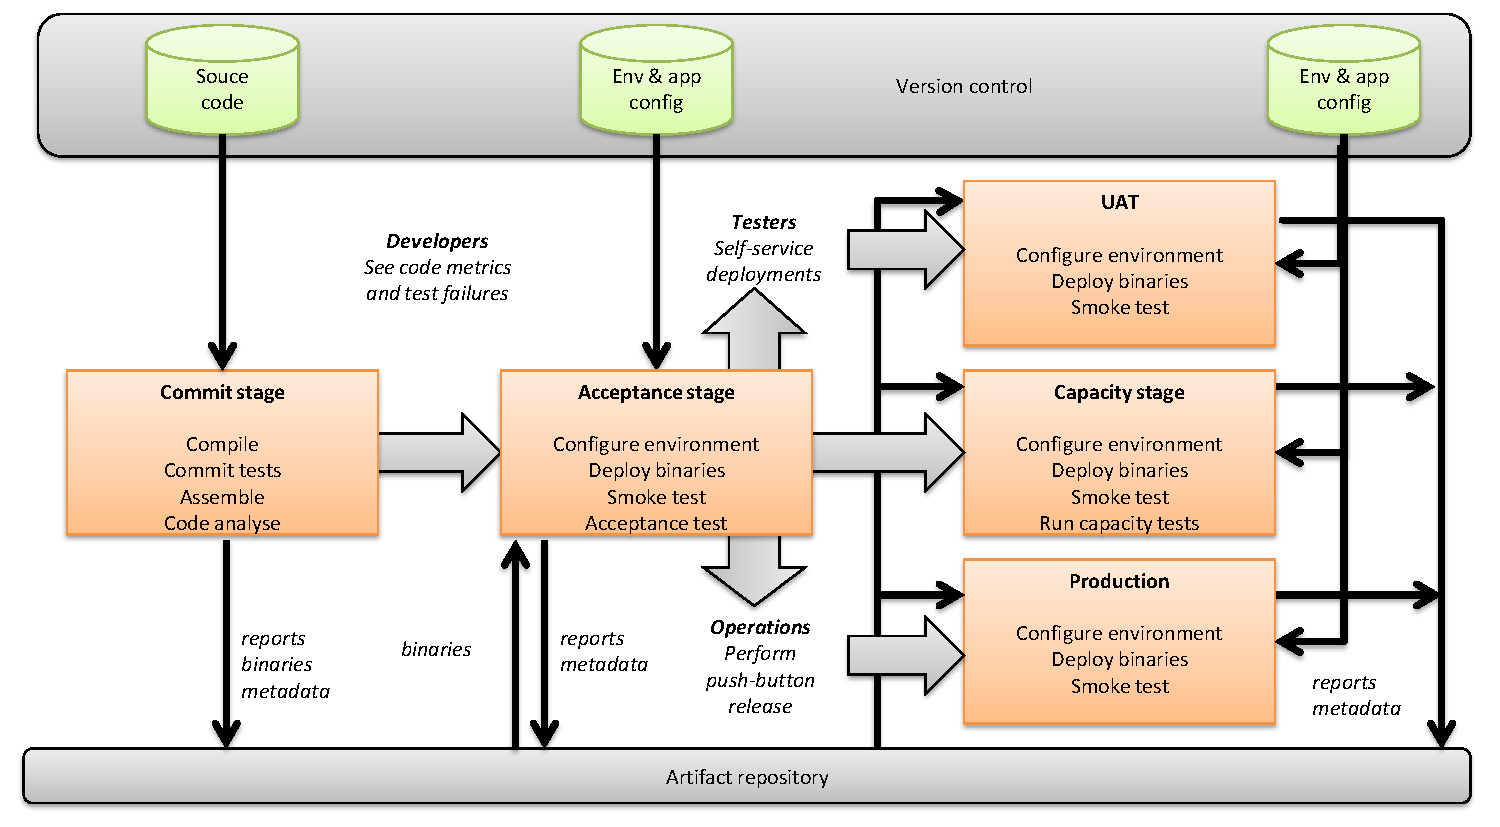
\includegraphics[width=.95\linewidth]{Grafiken/Delivery_Pipeline.pdf}}
\quelle{nach \cite[S. 111]{CD}}
\caption[Delivery Pipeline]{\dpipe\ nach \hf .}\label{pic:delivery_pipeline}
\end{figure}

\hf\ schlagen bei der Realisierung der \dpipe\ ein phasenweises Vorgehen vor und nutzen hierf�r den Begriff des \emph{Staging}.  Eine \emph{Stage} bildet eine deutlich abgrenzbare Phase ab. F�r die Umsetzung der \dpipe\ sollen diese nur der Orientierung einer m�glichen Einteilung dienen. Je nach gestellten Anforderungen an den Lieferprozess, ergeben sich andere Abl�ufen und Strukturen und die \emph{Stages} m�ssen anders modelliert werden. Abildung~\ref{pic:delivery_pipeline} zeigt die \dpipe , wie \hf\ sie vorschlagen. Grundlegende Elemente sind demnach:\footnote{Vgl. \cite[S. 109-110]{CD}}

\begin{itemize}
\item \comstage ,
\item \acstage ,
\item \uastage ,
\item \capstage\ und 
\item \prodenv .
\end{itemize}

\subsection{Die \comstage}

Die \comstage\ ist ein Prozess aus \ci . Sie stellt sicher, dass das entwickelte System sich auf dem erforderlichen technischen Niveau befindet. Das bedeutet, dass der Quellcode kompiliert und es keine Compiler-Fehler gibt, die die Komponententests fehlerfrei durchlaufen und die statische Analyse des Quellcodes eine hohe Testabdeckung und die Einhaltung von Programmierstandards bescheinigen.\footnote{Vgl. \cite[S. 109-110]{CD}}

Eine �nderung an der Quellcode-Basis im Versionsverwaltungssystem startet die \comstage . Das CI-System reagiert mit einer neuen Instanz des Integrationsprozesses und kompiliert sowie testet dabei den neuen Softwarestand. Dem Entwicklungsteam sollte ein Feedback �ber den aktuellen Zustand des Quellcodes nach ca. f�nf Minuten geben werden k�nnen. Nimmt dieser Prozess mehr Zeit in Anspruch, empfehlen \hf\ die Aufteilung der Unteraufgaben. Komponententests k�nnen \zb\ auch in parallel laufende Tasks aufgeteilt werden und auf verteilten Systemen ausgef�hrt werden. Die Ergebnisse k�nnen anschlie�end zusammengefasst und vom Entwicklungsteam ausgewertet werden.\footnote{Vgl.  \cite[S. 105-120]{CD}}

Metriken der statischen Codeanalyse, die in dieser Phase getestet werden, sind:\footnote{Vgl. \cite[S. 121]{CD}} 

\begin{itemize}
\item Testabdeckung, 
\item die Pr�fung auf Codedubletten, 
\item die zyklomatische Komplexit�t,
\item die Untersuchung nach der afferenten und efferenten Kopplung,
\item Warnungen und Programmierrichtlinien (\emph{Code Style}).
\end{itemize} 

Werkzeuge wie Sonar\footnote{Weitere Informationen zu Sonar unter \url{http://www.sonarsource.org/}.} verdichten die Testabdeckung auf einen prozentualen Wert. Dieser wird durch die Menge der im Test durchlaufenden Kontrollflusspfade bzw. der abgedeckten Codezeilen ermittelt. Wenn \zb\ bei der Menge der Eingaben, mit denen getestet wird, in einer Fallunterscheidung nie der alternative Zweig der Fallunterscheidung erreicht wird, betr�gt die Testabdeckung f�r dieses Konstrukt $50 \%$.\footnote{Vgl. \cite{sonar_testcoverage}}

Die zyklomatische Komplexit�t wird durch die zyklomatische Zahl ausgedr�ckt. Diese misst die strukturelle Komplexit�t des Quellcodes durch einen Kontrollflussgraph. Dabei wird die Menge unabh�ngiger Pfade im Programmablauf betrachtet.\footnote{Vgl. \cite[S. 100 f]{sl_basiswissen_sw_test}}

Mit der afferenten Kopplung wird die Anzahl der Pakete beschrieben, die von Klassen innerhalb des untersuchten Paketes abh�ngen. Efferente Kopplung hingegen beschreibt das Gegenteil, die Anzahl von Klassen eines Paketes die von Klassen au�erhalb des untersuchten Paktes abh�ngig sind. Diese Werte erm�glichen eine Beschreibung der Stabilit�t der Software. Demnach ist Stabilit�t $I = \frac{Ce}{Ca + Ce}$. Wobei $I$ im Intervall $[0,1]$ liegt, $Ce$ f�r efferente und $Ca$ f�r afferente Kopplung steht. Ein Wert von $0$ deutet auf Stabilit�t und darauf hin, dass dieses Pakte haupts�chlich von anderen benutzt wird. Dies k�nnte \zb\ f�r eine Schnittstellenbeschreibung der Fall sein oder auf einen Service hindeuten, der von anderen Paketen verwendet wird. Ein Wert von $0,5$ weist auf eine wechselseitige Beziehung zwischen den Paketen hin. Ein Wert von $1$ zeigt eine deutliche Abh�ngigkeit von anderen Paketen. �ndern sich die verwendeten Pakete, wird dieses auch Auswirkungen auf die Funktionsweise des untersuchten Paketes haben.\footnote{Vgl. \cite[S. 23-24]{martin_design_principles}}

Eine von Sun f�r die Programmiersprache Java empfohlene \emph{Code-Style}, also die Einhaltung von Programmierstandards, macht Vorgaben f�r die Organisation von Dateien, die Einr�ckungen im Quellcode, das Setzen von Kommentaren, die Deklaration von Variablen und die Vergabe von Namen. Ein Entwicklungsteam kann dabei weitere Richtlinien definieren. Ein verabredeter Standard unterst�tzt die Zusammenarbeit und erh�ht die Wartungsfreundlichkeit. Deren Einhaltung l�sst sich auf der Ebene der Entwicklungsumgebung sowie durch das CI-System in Form der statischen Code-Analyse pr�fen.\footnote{Vgl. \cite{java_code_conv}}

Ein CI-System sollte Artefakte wie Test-Protokolle und Binaries in einem zentralen Verzeichnis, einem Repository, verwalten k�nnen. Das ist notwendig, da nachfolgende Phasen auf diesem Ergebnis aufbauen und die Binaries in der \acstage , \uastage , \capstage\ und in \prodenv , dem Produktivsystem, wiederverwenden.

Die in der \comstage\ erstellten Softwarepakete sollten in einer sp�teren Phase nicht noch einmal kompiliert werden. Es k�nnte sonst nicht zweifelsfrei und revisionssicher garantiert werden, dass die dann gelieferte Version auch der getesteten exakt entspricht. Flexibilit�t und Wartbarkeit werden reduziert, wenn f�r bestimmte Umgebungen spezielle und angepasste Binaries erstellt werden m�ssen.\footnote{Vgl.  \cite[S. 113]{CD}}

\subsection{\acstage , \uastage , \capstage\ und \prodenv}

Ob ein \rc\ auch in die Produktivumgebung ausgeliefert werden kann, ist in der \comstage\ noch nicht endg�ltig entscheidbar, da hier nur die technische Funktion �berpr�ft wird. Eine Softwareversion in die Produktivumgebung zu bringen, setzt die Abnahme des Werkes und damit die Erf�llung der spezifizierten Akzeptanzkriterien aus den funktionalen und nicht-funktionalen Anforderungen voraus. 

Die \acstage\ pr�ft auf der Seite des Lieferanten, ob diese Anforderungen erf�llt werden und das Verhalten der Anwendung die Bed�rfnisse des Nutzers erf�llt und der Spezifikation gerecht wird. Bei den nicht-funktionalen Anforderungen wie \zb\ den Kapazit�tstests sollte eine Auslagerung der Tests als eigene Stage, der \capstage , vorgenommen werden. Die Pr�fung der Anwendung auf m�gliche Auslastungsengp�sse l�uft gew�hnlich l�nger und sollte deshalb parallelisiert werden.\footnote{Vgl. \cite[S. 124-128]{CD}}

\cd\ setzt voraus, dass alle Testf�lle f�r jede neue Version der Quellcode-Basis durchlaufen werden. Damit kann der Quellcode auch auf Regression getestet werden und eine Verschlechterung der Qualit�t so schnell erkannt werden. Eine zuvor funktionierende Software, die nach einer �nderung bestimmte Qualit�tskriterien nicht mehr erf�llt, kann schnell identifiziert und durch das Entwicklungsteam unverz�glich angepasst werden, damit diese Anforderungen wieder erf�llt werden.

F�r die Verifizierung von Akzeptanz- und Kapazit�tskriterien muss die Software in einer Umgebung ausgef�hrt werden, welche der Produktivumgebung entsprechen soll. Wenn Struktur und Konfiguration dieser Umgebungen zu sehr von denen der Produktivumgebung abweichen, kann nicht ausgeschlossen werden, dass es im Produktivsystem zu einem nicht vorhersehbaren Verhalten kommt. Handelt es sich beim Produktivsystem \zb\ um ein komplexen und teuren Server-Cluster, wird es wirtschaftlich nicht m�glich sein, die Produktivumgebung exakt nach zu bilden. Im Fall des Server-Cluster kann aber ein herunter skaliertes System f�r den Test bereitgestellt werden. Die Lasttests k�nnen entsprechend dem Verh�ltnis von Test- und Produktivumgebung skaliert werden.

Mit der \uastage\ wird f�r jede Softwareversion ein Pilotbetrieb der Anwendung umgesetzt. Wird die Software durch einen externen Dienstleister als Werk erbracht, f�hrt, sofern nicht anders vereinbart, das Ausliefern der Anwendung in die Produktivumgebung zur Abnahme des Werkes durch den Auftraggeber. Eine direkte Auslieferung nach jedem m�glichen Commit eines Entwicklers ist in dieser Konstellation nicht m�glich. Werden aber vertragliche Teillieferungen vereinbart, ist auch die Abnahme nur einen Teil, der im Gesamtpakt vereinbarten Funktionalit�ten m�glich, sodass die Abnahme des Werkes erst am Ende der Vertragslaufzeit endg�ltig vollzogen wird.

Die letzte Stufe im Liefersystem bildet die Auslieferung einer gut getesteten und den Anforderungen entsprechenden Version der Software in die Produktivumgebung. Ein Versagen in einer Teilphase verneint die Lieferf�higkeit der inspizierten Version. \hf\ schlagen f�r das Deployment eines \rc\ ein \ssp\ vor. Von diesem aus k�nnen die Beteiligten im Lieferprozess die F�higkeit erhalten, den Liefervorgang selbst ansto�en zu k�nnen. So kann ein Release-Manager dem Kunden die vereinbarte Version in seine Testumgebung liefern, damit dieser die Werkabnahme vollziehen kann. Die Entscheidung, das abgenommene Werk in das Produktionssystem auszurollen, tr�gt der Kunde dann selbst. Dieser Vorgang kann ihm durch die Bereitstellung eines speziell vorbereiteten \ssp\ vereinfacht bzw., wenn entsprechend vereinbart, durch den Dienstleister nach vorhergehendem Auftrag durchgef�hrt werden.

\subsection{Skripte f�r Build und Deployment}

Eine Grundtechnik der \dpipe\ stellen Skripten und Konfigurationsdateien dar. Je nach verwendetem Betriebssystem, auf dem die \dpipe\ ausgef�hrt wird, k�nnen kleinere Programme in einer vom Betriebssystem unterst�tzten Skriptsprache verfasst werden, um die anfallenden Aufgaben bei der Systemkonfiguration und dem Deployment auszuf�hren. Mit Skripten k�nnen Programme und Informationen zur Steuerung und Organisation von Kompilier- und Verteilungsvorg�ngen verfasst werden. Beim Kompilieren von Quellcode stehen \zb\ im Bereich der Programmiersprache Java die Build-Tools Ant und Maven zur Verf�gung, deren Anweisungen, bei Ant, in der \texttt{build.xml} bzw. deren Konfiguration, bei Maven, in der \texttt{pom.xml} festgehalten werden. Zu den weiteren Aufgaben von Konfigurations- und Verteilungskripten geh�ren das Anpassen der Datenbank an neue Erfordernisse, das Deployen der neuen Softwareversion sowie das Installieren und Konfigurieren ben�tigter Middleware, Diensten und Komponenten. Das Verfassen von Skripten sollte dabei aber eine Aufgabe sein, die von Entwicklern und IT-Betrieb in gemeinsamer Verantwortung durchgef�hrt wird.\footnote{Vgl. \cite[S. 147-150, 161]{CD}}

\hf\ sehen hier drei M�glichkeiten, um die Konfigurations- und Verteilungsscripte auf dem Zielsystem automatisiert auszuf�hren:

\begin{itemize}
\item Ein Script, welches auf dem System der \dpipe\ aufgerufen wird, sich mit der gew�nschten Plattform verbindet und die entsprechenden Kommandos zur �nderung absetzt. Bei Unix-Betriebssystemen kann hier \zb\ das SSH-Protokoll genutzt werden, um Befehle �ber eine gesicherte Verbindung auf einem Remote-System ausf�hren zu k�nnen.
\item Ein Konfigurationsskript wird auf einem Verwaltungsserver bereit gestellt. Auf der Zielplattform l�uft ein Agent, der sich mit dem Server verbindet und das Konfigurationsskript l�dt und ausf�hrt. Ein derartiges Konzept setzt das Werkzeug Chef\footnote{Mehr Informationen zu Chef unter: \url{http://www.opscode.com/chef/}} von Opscode um. Chef kann auf diese Weise einen ganzen Infrastruktur-Cluster verwalten und eine �nderung an der Systemkonfiguration durchf�hren und ben�tigte Software installieren.
\item Durch das Ausnutzen des Paketsystems der jeweiligen Zielplattform kann \zb f�r Debian Paketsystem \emph{dpkg} ein Paket erstellt werden, welches die auszuliefernden Binaries enth�lt sowie ein \emph{control file} der Informationen �ber die Pakete enth�lt, von denen die zu installierende Software abh�ngt sowie in Konflikte steht. Die Ausl�sung von Abh�ngigkeiten �bernimmt dann das Debian Package-Tool.\footnote{Vgl. \cite{Brockmeider2003}}
\end{itemize}

\section{Kritische Komponenten im Liefersystem}

\subsection{Datenbanken in der \dpipe}

Datenbanken im Liefersystem ben�tigen eine besondere Aufmerksamkeit w�hrend des Softwarerelease. Dies gilt, sofern die Struktur der verwendeten Datenbank durch ver�nderte Anforderungen an das Gesamtsystem angepasst werden muss. Kann zu Beginn einer Entwicklung davon ausgegangen werden, dass es keine �nderungen am Datenbankschema geben wird, weil ein System entwickelt wird, welches sich an der Struktur einer bestehenden Datenbank ausrichten soll, bedarf dieses Thema keiner weiteren Beachtung. 

Anders verh�lt es sich, wenn die Datenbank ausschlie�lich von einer Anwendung genutzt wird und das Schema der Datenbank den neuen Anforderungen und Funktionalit�ten angepasst werden muss. So k�nnte eine neue Funktionalit�t in einer Webanwendung \zb\ das Anlegen einer neuen Tabelle in der Datenbank erfordern oder die Anpassung von bestehenden Datenbankeintr�gen. Der Verlust von Daten kann dabei aber nicht hingenommen werden.  Der Aktualisierungsvorgang erfordert deshalb die gleiche Aufmerksamkeit, wie die Aktualisierung der Anwendung selbst.

Wird eine Anwendung inkrementell aktualisiert, \zb\ Server eines Clusters nacheinander, kann es dabei zu Problemen kommen, wenn in den Clustern unterschiedliche Datenbankversionen von den laufenden Anwendungen genutzt werden. Transaktionen mit der alten Datenbank, die w�hrend des Aktualisierungsvorgangs von der alten Softwareversion durchgef�hrt werden, m�ssen nach Abschluss des Aktualisierungsvorgangs auch in die neue Datenbank �bertragen werden. Ein Datenverlust muss vom Release vermieden werden.

Schwierig kann es aber auch sein, ein Rollback auf die alte Version durchzuf�hren. Transaktionen, die mit der neuen Softwareversion auf die aktualisierte Datenbank durchgef�hrt wurden, m�ssen bei einem Rollback in die alte Datenbankversion �bertragen werden. Hier stellt sich die Frage, was mit Daten geschehen soll, die nicht mit dem alten Datenbankschema kompatibel sind.

\hf\ schlagen hier folgendes Vorgehen vor:\footnote{Vgl. \cite[S. 328-333]{CD}}

\begin{description}
\item[Inkrementelle �nderungen: ] Zu Beginn der Entwicklung wird eine neue leere Datenbank aufgesetzt. Werden Tabellen ben�tigt oder m�ssen angepasst werden, k�nnen die ben�tigten Anweisungen durch ein Skript ausgef�hrt werden. Das Skript enth�lt auch Anweisungen f�r das Rollback der �nderungen. Im Skript selbst sind Informationen enthalten, von welcher Datenbankversion auf welche aktualisiert wird. Die aktuelle Version der Datenbank kann in der Datenbank selbst gespeichert werden. Die \dpipe\ kann so programmatisch pr�fen, ob die vorgesehenen �nderungen auch ausgef�hrt werden d�rfen. Im Zweifelsfall bricht der Vorgang ab. Bevor die \dpipe\ �nderungen durchf�hrt, m�ssen alle Bedingungen gepr�ft und erf�llt sein.
\item[Datenbank-Rollback: ] Geht ein Deployment schief, muss die alte Datenbank wieder hergestellt werden k�nnen, ohne in der Zwischenzeit durchgef�hrter Transaktionen verlustig zu werden. Daf�r muss vor einem Deployment ein Back-up der Datenbankdateien erstellt und auf einem zweiten Datenbankserver bereitgestellt werden. Anschlie�end k�nnen die �nderungen an an dem Datenbankserver vorgenommen werden, auf den die Anwendung nicht zugreift. Die korrekte Funktionsweise der Datenbank ist anschlie�end zu testen. Die Anwendung kann nun, \zb\ in einem Cluster, st�ckweise herunter gefahren, aktualisiert und wieder hochgefahren werden. Die neue Version der Software greift auf die neue Datenbank zu, die alte Software auf die alte Datenbank. Um den Vorgang abzuschlie�en, wird am Ende des Vorgangs ein Delta der alten Datenbank zwischen Update-Beginn und Update-Ende in die neue Datenbank �bertragen.
\item[Entkopplung von Anwendungs- und Datenbankupdate: ] Die Entkopplung von Datenbank- und Anwendungsupdate erfordert ein mehrstufiges Vorgehen. Soll von einer Version auf die andere aktualisiert werden und die neuere Version ben�tigt \zb\ eine neue Tabelle, muss dies vor dem Anwendungsupdate durchgef�hrt werden. Die neue als auch die alte Anwendungsversion m�ssen dann mit der ge�nderten Datenbank kompatibel sein. Werden Tabellen nach einem Anwendungsupdate nicht mehr genutzt und sollen entfernt werden, kann dies erst nach dem erfolgreichen Anwendungsupdate erfolgen. In Abbildung~\ref{pic:db_deploy} wird dieses Vorgehen visualisiert. Sind gr��ere �nderungen des Datenbank-Schemas notwendig, um \zb\ ein neues Feature zu realisieren, m�ssen die �nderungen am Quellcode die Einschr�nkungen durch die Datenbank ber�cksichtigen und in kleine Schritte zerlegt werden. Die Auswirkungen auf die aktive Datenbank k�nnen dann so gering wie m�glich gehalten werden.
\end{description}

\begin{figure}
\centering
\fbox{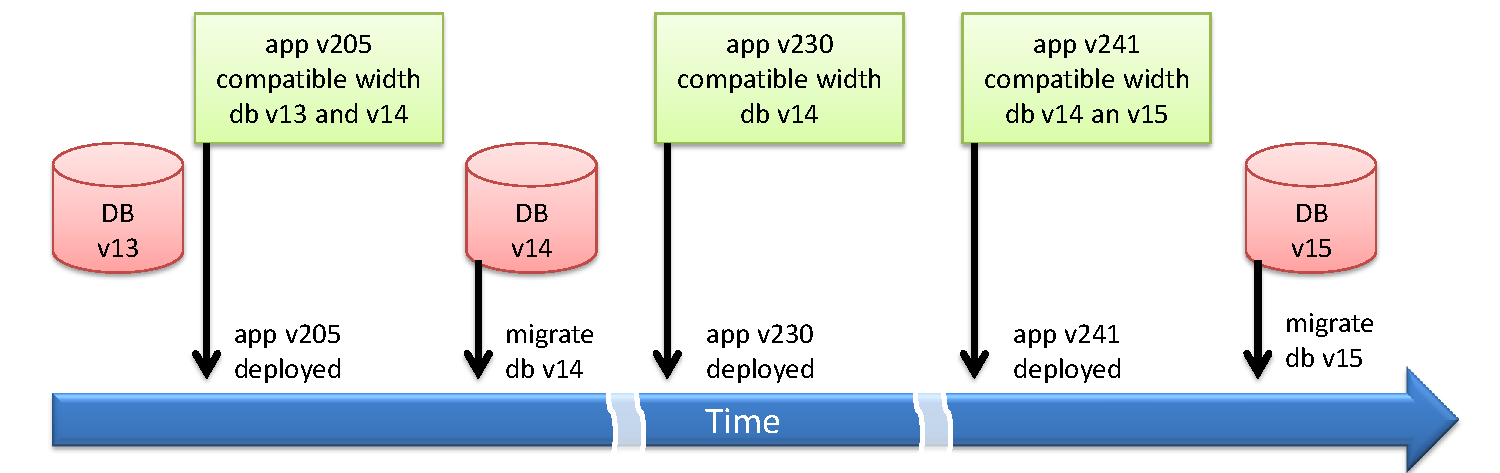
\includegraphics[width=.95\linewidth]{Grafiken/db_deploy.pdf}}
\quelle{nach \cite[S. 333]{CD}}
\caption[Datenbank-Migration]{Datenbank-Migration in der \dpipe.}\label{pic:db_deploy}
\end{figure}

Die besonderen Erfordernisse von Datenbanken m�ssen bei der inkrementellen Anwendungsaktualisierung ber�cksichtigt werden. Ein Release sollte dabei so gestaltet werden, dass nur marginale �nderungen an einer produktiv eingesetzten Datenbank durchgef�hrt werden m�ssen. Die Integrit�t der Daten darf nicht gef�hrdet werden. Sind gr��ere �nderungen an der Datenbank notwendig, um eine neue Funktionalit�t zu erm�glichen, ist es eventuell m�glich, aus einem gro�en Release mehrere kleine Schritte zu machen Die Auswirkung auf die Datenbank kann so reduziert werden.

\subsection{Strategien f�r die Versionsverwaltung}

Die Funktionalit�ten des Versionsverwaltungssystems, \emph{Branch} und \emph{Merge}, nehmen auf die Funktionsf�higkeit einer \dpipe\ Einfluss. Mit einem Branch wird ein paralleler Entwicklungszweig begonnen. Dies ist \zb\ notwendig um eine parallele Entwicklung eines Features zu erm�glichen, ohne den Hauptast oder andere Entwicklungen negativ zu beeinflussen, bis das Feature umgesetzt ist.\footnote{Vgl. \cite[S.154-159]{popp_konfig}}

Eine Folge dessen ist ein erh�hter Integrationsaufwand beim \emph{Merge}, bei dem ein Zweig in den Hauptstamm integriert wird. Je gr��er diese Differenzen, desto gr��er der Aufwand des Zusammenf�hrens. \hf\ empfehlen, einen Zweig nach ein bis maximal zwei Tagen wieder in den Hauptstamm zu integrieren. Zudem wird der Zweig nicht mehr von der \dpipe\ erfasst. Ein Feedback �ber den Zustand des Quellcodes ist f�r den Zweig nicht m�glich.\footnote{Vgl.  \cite[S. 390-393]{CD}}

\section{Implikationen f�r das Liefersystem}\label{lierfsys_implikation}

Aus den Konzepten von \cd\ und Vorschl�gen f�r die Umsetzung einer \dpipe\ ergeben sich folgende Implikationen f�r ein Liefersystem:

\begin{itemize}
\item Das Liefersystem besteht aus Infrastruktur und Systemumgebungen. Es hat Auswirkung auf das Entwicklungsteam und auf den IT-Betrieb. Beide Gruppen m�ssen eng zusammenarbeiten, um eine automatisierte, \dpipe\ realisieren zu k�nnen. \devops\ schl�gt hierf�r gemischte Entwicklungsteams vor, die Kompetenzen aus beiden Bereichen besetzen k�nnen.
\item Das Liefersystem gibt allen Beteiligten ein Feedback. Hierzu geh�ren der aktuelle und der historische Zustand der Quellcode-Basis, welche Version in welcher Umgebung ausgef�hrt wird sowie aktuelle Vorg�nge in der \dpipe .
\item Das Liefersystem wird in Phasen unterteilt. Die Qualit�tssicherung wird weitgehend automatisiert. Das Scheitern einer Phase stoppt die Instanz der \dpipe\ und damit alle nachfolgenden Phasen.
\item Das Liefersystem baut auf \ci\ auf und erweitert das Konzept um ein automatisiertes Deployment.
\item Das Liefersystem muss sich um die Konfiguration der Infrastruktur k�mmern und diese �berwachen. Hierf�r sind Skripte zu erstellen, welche die notwendigen �nderungen an der Ausf�hrungsumgebung vornehmen k�nnen.
\item Das Liefersystem stellt eine Oberfl�che bereit, welche das Deployment einer Version in eine Testumgebung oder in die Produktionsumgebung auf eine einfache Weise ansto�en kann. Ansto�en bedeutet, das Deployment-Skript auszuf�hren. Als Methode gen�gt eine schlichte Oberfl�che mit einem einfachen Push-Button dessen Bet�tigung zur Ausf�hrung des Skripts f�hrt.
\item Das Liefersystem muss f�r Komponenten wie Datenbanken ein geeignetes Konzept bereithalten, um �nderungen und Rollback ohne Verlust von Daten verwirklichen zu k�nnen. Zweige in der Versionsverwaltung umgehen das Liefersystem und sollten vermieden werden.
\item Das Liefersystem muss stetig weiter entwickelt werden und sich den Anforderungen anpassen k�nnen.
\end{itemize}

\cd\ und die \dpipe\ ben�tigen spezielle Werkzeuge. Dabei ist es f�r die Ausf�hrung unerheblich, ob es ein einzelnes Werkzeug gibt, mit dem alle Anforderungen erf�llt werden k�nnen oder eine Verkn�pfung von verschiedenen Werkzeugen und Scripten zu einer \emph{Tool chain} das Gleiche Ergebnis liefert. 

\comment{Wie ist der derzeitige Entwicklungsstand von \cd\ bei adesso und welche Technologien f�r die Auslieferung von Software werden derzeit verwendet? Hierzu ist ein typisches Web-Projekt hinsichtlich seiner Auslieferung zu untersuchen. Welche Auslieferungsverfahren f�r Web -Anwendungen gibt es? Der Entwicklungsstand ist eine Voraussetzung, um sp�ter Beurteilen zu k�nnen, welches Werkzeuge f�r adesso geeignet ist, weil es sich beispielsweise gut in die bestehende Infrastruktur integrieren l�sst.}

\chapter{Entwicklungsstand von \cd\ bei adesso}

%\comment{Was ist am Entwicklungsstand interessant, warum soll dieser untersucht werden?}

Dieser Abschnitt geht auf die derzeitige Situation der Auslieferung von Software bei adesso ein. Hierzu geh�ren der Auslieferungsprozess und die Infrastruktur, die f�r die Auslieferung bereitsteht. Dies ist notwendig, um Ansatzpunkte f�r die noch zu untersuchenden Werkzeuge zu finden.

adesso als unabh�ngiger IT-Dienstleister ber�t und entwickelt individuelle Software f�r Kunden aus den Branchen Versicherungen und R�ckversicherungen, Banken und Finanzmarkt, Gesundheitswesen, Lotterie, �ffentliche Verwaltung, Telekommunikation und Medien.\footnote{Vgl. \cite{ad_branchen}} Jeder Kunde hat dabei bestimmte Anforderungen und Rahmenbedingungen, die er an die Projekte kn�pft. Mit einer heterogenen Projektlandschaft hinsichtlich der eingesetzten Verfahren, Technologien oder Prozesse wird nicht zu rechnen sein. Zudem wird angenommen, dass es bei adesso schon parallel Bem�hung gibt, den Auslieferungsprozess zu verbessern bzw. \cd\ zu erm�glichen.

\section{Ausgangssituation f�r die Untersuchung des Entwicklungsstandes}

%\comment{Wird ben�tigt um das Betriebsszenario f�r die zu untersuchenden Werkzeuge genauer zu beschreiben. In der Einleitung muss schon erw�hnt werden, dass adesso haupts�chlich Web-Projekte im Java realisiert. Hier soll noch einmal ausf�hrlicher dargestellt werden, wie die Projekte genau aufgebaut sind. Diese sollte am bestem am Beispielprojekt erfolgens, an dem sp�ter die Deployment Pipeline realisiert wird. Dies ist aber nur einleitend f�r das anschlie�ende Kapitel und dient der allgemeinen Erhellung, dass es sich um Web-Projekt aus dem Java-Umfeld handelt f�r z.B. Kunden aus dem Versicherungs- bzw. Banken-Umfeld.}

%\comment{Technologieumfeld bei adesso und Zielprojekte}

%\TODO{Doppelnennungen! Absatz �berarbeiten und Bezug zur Einleitung herstellen.}

Technologisch unterscheidet adesso Projekte selbst nach den Kategorien Java, Microsoft, Mainframe sowie Enterprise Content Management.\footnote{Vgl. \cite{ad_tech}} Bei der weiteren Betrachtung des aktuellen Auslieferungsprozesses sowie von \cd\ sollen vornehmlich Projekte aus dem Java bzw. JEE-Umfeld und Web-Umfeld betrachtet werden. Das ist der Bereich, bei dem im Unternehmen eine hohe Aktivit�t und ein besonderes Interesse an neuen Ans�tzen wie \cd , Behavior Driven Develpment (kurz BDD), Big-Data und Cloud-Computing herrscht.\footnote{Vgl. \cite{ad_cloud}} 

Auf technischer Ebene l�sst sich ein kontinuierliches Ausliefern von Software mit verschiedenen Plattformen und Softwarearchitekturen verwirklichen, im Zentrum der weiteren Betrachtung stehen hier aber  Web-Anwendungen. H�ufig werden WAR und EAR-Files f�r Web- und Applikations-Container nach der JEE-Spezifikation entwickelt.\footnote{Weitere Informationen zur JEE-Sepzifikation: Vgl. \cite{javaee_spec}}

%\comment{CI-Team und Infrastruktur}
%\TODO{Integratiosf�higkeit der Werkzeuge sowie Prozesse mehr in den Vordergrund r�cken!}

Um Projektrisiken durch sp�te Integration einzelner Softwarekomponenten zu reduzieren, stellt adesso ein System f�r \ci , kurz CI-System genant, bereit. Dort k�nnen Projektteams den aktuellen Stand ihrer Software automatisiert kompilieren und die Komponenten testen lassen. Besonders bei modularen Softwaresystemen, ist die Integration von mehreren Softwareteilen eine mit hohen Aufw�nden verbundene Angelegenheit.

Damit die Konfiguration des CI-Systems f�r ein neues Projekt reibungslos ablaufen kann, stellt adesso den Projektteams ein Support-Team bereit. Dieses ist mit Spezialisten rund um das Thema \ci\ und Build-Management besetzt. Hauptgrund, ein solches Support-Team zu unterhalten, ist die stetige Wiederholung von Aufgaben, die beim Einrichten eines neuen Projektes anfallen. Das adesso Build-Management stellt eine gemeinsame Integrations- und Test-Umgebung bereit. Zudem k�nnen sich Projektteams zu Technologien beraten lassen, die das Build-Management betreffen. Ziel einer Beratung ist die geeignete Wahl eines Build-Werkzeugs und die Erarbeitung von Build-Skripten. Vordergr�ndig werden dabei die Werkzeuge Ant und Maven unterst�tzt.\footnote{Vgl. \cite{ad_build}}

%\comment{Grund f�r die Untersuchung des IST-Zustandes?}

%\TODO{Warum dieses Reifegradmodell?}

Wieweit der derzeitige Prozess ausgereift ist und die noch zu untersuchenden Werkzeuge erg�nzt werden k�nnen, muss die Untersuchung des Istzustandes zeigen. Durch den Einsatz eines Reifegradmodells soll sich der derzeitige Entwicklungsstand absch�tzen und beurteilen lassen. Ein Reifegradmodell f�r \ci\ und \cd\ wurde von der Firma UrbanCode\footnote{Mehr Informationen zu UrbanCode: \url{http://www.urbancode.com/}} ver�ffentlicht, die sich auf die Entwicklung von Werkzeugen zur Unterst�tzung von DevOps und \cd\ spezialisiert hat. Da sich UrbanCode auch auf Werkzeuge f�r \cd\ anbietet, dient das Modell auch zu einem Teil der Eigenwerbung. In seinem Ansatz kann es aber unabh�ngig genutzt werden, um den eigenen Zustand im Unternehmen zu beschreiben.

%\comment{Ziel von CD und Nutzen f�r adesso}

%\TODO{Wird schon in der Problemstellung von CD beschrieben!}

Ein Hauptanliegen von \cd\ ist die Ausbeutung von Gewinnchancen, die durch die kurzen Iterationen agiler Vorgehensmodelle entstehen. Wenn neu entwickelte Programmfunktionalit�ten unverz�glich am Markt angeboten oder in Unternehmensanwendungen eingesetzt werden k�nnen, ergeben sich hieraus strategische Vorteile f�r das Unternehmen gegen�ber anderen Wettbewerbersteilnehmern. Damit adesso seinen Kunden einen solchen Vorteil anbieten kann, m�sste der Auslieferungsprozess auf diese Zielstellung angepasst sein.

\section{Erhebungsmethode zum Entwicklungsstand}

%\comment{Ein Einstiegspunkt f�r die Analyse, wie \cd\ den Auslieferungsstand konkret verbessern kann. Hieraus kann dann auch abgeleitet werden, warum es (m�glicherweise) effektiver ist, \cd\ und eine Deployment Pipeline im Auslieferungsprozess einzusetzen.}

%\comment{Ziel einer Erhebung}

% ! OLD
% Wie in einem adesso-Projekt derzeit fertiggestellte Software ausgeliefert wird, kann durchaus unterschiedlich und an die Rahmenbedingungen des beauftragenden Kunden gebunden sein. Mit dem adesso CI-Team steht ein Ansprechpartner bereit, der �ber umfassende Kenntnisse der verwendeten Verfahren und Systeme Auskunft geben und somit eine den derzeitigen Stand der Auslieferungspraxis darlegen kann.

%\comment{M�glichkeiten einer Erhebung}

Neben der Recherche der unternehmensinternen Quellen besteht durch das CI-Team die Gelegenheit, einzelne Mitarbeiter zur aktuellen Praxis bei der Auslieferung von Software zu befragen. Die Befragung des CI-Teams kann als Einzelinterview oder in Form eines Fragebogens erfolgen. Ein Einzelinterview bietet dabei die M�glichkeit einer individuell gef�hrten Befragung. Im Gegensatz dazu legt ein Fragebogen einen gleichbleibenden Befragungsrahmen fest und kann zudem den Zeitaufwand der Befragung f�r den Fragesteller sowie f�r den Befragten auf ein Minimum reduzieren.

Um den Zeitaufwand so gering wie m�glich zu halten, wird auf den Fragebogen als Erhebungsinstrument zur�ckgegriffen. Der Fragebogen kann dabei so gestaltet werden, dass sich der Befragungsaufwand f�r die Befragten auf einen Zeitaufwand von 10 bis 15 Minuten reduzieren l�sst. Der Aufwand, die formulierten Fragen �ber ein Telefoninterview zu vermitteln und die Antworten zu notieren, wird auf 45 bis 60 Minuten gesch�tzt.

Zudem kann der Fragebogen zu einer beliebigen Zeit beantwortet werden und so die individuelle Koordination eines Gespr�chstermins mit den Mitgliedern des CI-Teams umgangen werden. Der Fragebogen selbst dient keiner statistischen Auswertung. Vielmehr sollen mit ihm die Meinungen und Standpunkte der Befragten eingesammelt werden.

%\comment{Welche Fragemethoden werden eingesetzt}

Bei der Gestaltung des Fragebogens werden nur zu einem geringen Teil freie Textfelder verwendet. Mehrheitlich ist der Fragebogen so konzipiert, dass der Befragte bestimmten Aussagen zustimmen oder diese ablehnen kann. Zu jeder Frage gibt es weiterhin die M�glichkeit, freie Anmerkungen zu geben. Hierdurch k�nnen auch Ideen zu bestimmten Themen durch die Befragten ge�u�ert werden, wie es auch in einem Telefoninterview m�glich w�re.

%\comment{Herkunft der Fragen}
%\comment{Warum sind die Pattern und das Maturity Model f�r den Fragebogen geeignet.}

Als Grundlage des Fragebogens werden das \emph{Enterprise Continuous Integration Maturity Model} von UrbanCode\footnote{Vgl. \cite{cd_maturitymodel}} sowie die von \hf\ entwickelten Konzepte zu \cd\footnote{Vgl. \cite{CD}}\ genutzt. Das Maturity-Model f�r \cd\ wurde f�r eine Selbstevaluierung von Unternehmen entwickelt. Dabei werden Zielvorgaben definiert, an denen sich die Reifegrade bestimmen lassen. Untergliedert ist das Modell in die Einheiten Kompilieren, Ausliefern und Testen einer Anwendung sowie die Berichtserstellung und Visualisierung des Prozesses.

%\TODO{Maturity-Model darstellen!}

Der Fragebogen ist Unterteilt nach \comstage , \acstage und \emph{Deployment}. Dieser orientiert sich damit an der von \hf\ vorgeschlagenen Struktur der \dpipe.\footnote{Vgl. \cite[S. 111]{CD}} Zus�tzlich soll der Befragte zu Beginn die Phasen des Auslieferungsprozesses selbst skizzieren. Dies soll das Selbstverst�ndnis �ber die Phasen der \comstage\ zeigen.

Im Bereich der \comstage\ wird der Reifegrad des Build-Prozesses abgebildet und es werden Fragen zum Konfigurationsmanagement sowie zum Umgang mit Artefakten gestellt. Unter die \acstage\ fallen Fragen zu Verfahren und Werkzeugen, die beim Testen von Quellcode verwendet werden. Die letzte und kritische Phase der \dpipe\ ist das Ausrollen der Anwendung in die Produktivumgebung. Hierzu werden Fragen im Bereich des \emph{Deployments} gestellt. Es wird versucht zu ermittelt, welche Bem�hungen es bei adesso derzeit gibt, um eine \dpipe\ aufzubauen.

\section{Auswertung und Darstellung des Entwicklungsstandes}

%\comment{Ergebnisdarstellung des Fragebogen}

Der Fragebogen wurde von drei Mitarbeitern beantwortet, welche den repr�sentativen Kern des CI-Teams darstellen. Die konkreten Antworten k�nnen dem Anhang~\ref{anhang_entwicklungsstand} entnommen werden. In diesem Abschnitt werden die gegebenen Antworten ausschlie�lich zusammengefasst und im Zusammenhang mit \cd\ betrachtet.

Da sich nicht alle gegebenen Antworten decken, wird hieraus geschlussfolgert, dass es noch kein durchgehendes standardisiertes Vorgehen f�r den Auslieferungsprozess gibt und es vom jeweiligen Projekt abh�ngig ist, welche Phasen und Teilprozesse von \ci\ und \cd\ unterschieden und realisiert werden.

\subsection{Phasen des derzeitigen Entwicklungs- und Auslieferungsprozesses}

Aus dem Fragebogen gehen folgende Phasen des Entwicklungs- und Auslieferungsprozesses hervor:

\begin{itemize}
\item Aufsetzen der Projektumgebung und Einrichten der Entwicklungsumgebung,
\item Entwicklung der Software,
\item Durchf�hren von Integrationstests und
\item Auslieferung der Software.
\end{itemize}

\begin{figure}
\centering
\fbox{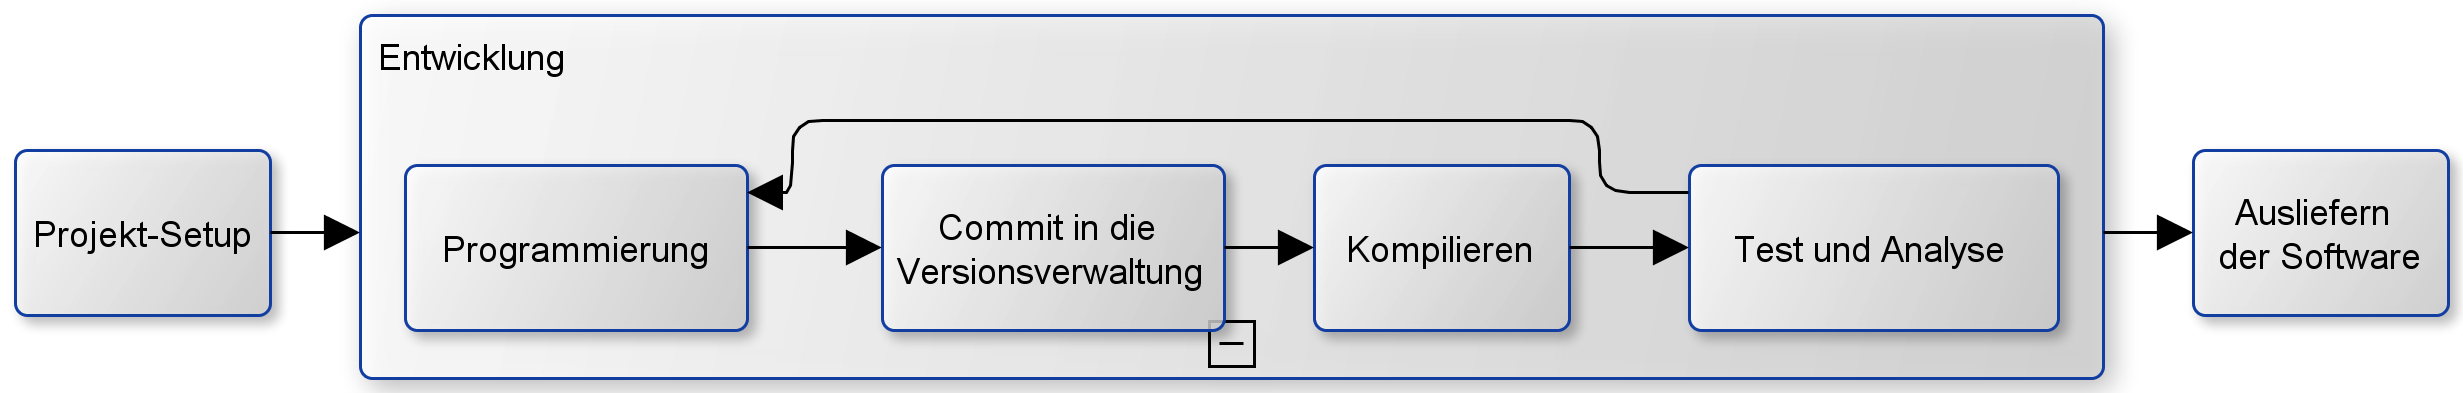
\includegraphics[width=\linewidth]{Grafiken/04_sw_prozess_adesso.PNG}}
\caption[Lieferprozess adesso]{Lieferprozess bei adesso.}\label{pic:sw_prozess_adesso}
\end{figure}

Die Entwicklung unterteilt sich in die Erstellung des Quellcodes und die anschlie�enden Phasen von Kompilierung, Tests und Analyse. Dieser Prozess wird durch die �nderung der Quellcode-Basis in der Versionsverwaltung als automatisierter Vorgang angesto�en. Abbildung~\ref{pic:sw_prozess_adesso} zeigt diesen Prozess. Optional ist ein automatisiertes Deployment in eine Testumgebung bzw. auf ein Staging-System. In dieser Umgebung k�nnen weitere Tests wie \zb\  Akzeptanz- oder Lasttests durchgef�hrt werden. Sind alle Phasen erfolgreich verlaufen, kann das Release durchgef�hrt werden und die Software in die Produktivumgebung installiert und ausgef�hrt werden.

Entwickelt wird zunehmend unter dem TDD-Ansatz, dem Test-Driven-Development. TDD setzt die Erstellung von Test-F�llen vor die Implementierung der Funktionalit�t. Ziel dieses Vorgehens ist die Fokussierung des Entwicklungsprozesses auf die noch umzusetzenden Funktionalit�ten. Deren erwartetes Ergebnis wird zu Beginn der Implementierung einer Funktionalit�t festgelegt.\footnote{Vgl. \cite{Ambler}}

Da es oftmals keinen direkten Zugriff auf die Produktivumgebung des Kunden gibt, kann \zb\ im JEE-Umfeld nur ein fertiges WAR- oder EAR-File ausgeh�ndigt werden. Die Anwendung wird mit einer Installationsanleitung �bergeben. Mitarbeiter des Kunden bzw. ein weiterer Dienstleister in Form eines Rechenzentrums ist dann f�r die Installation und den reibungslosen Betrieb der Anwendung verantwortlich. Besteht der direkte Zugriff auf die Produktivumgebung, \zb\ weil adesso selbst f�r den Kunden das System betreibt, sind automatisierte Auslieferungen in die Produktivumgebung m�glich.

\subsection{\comstage}

Kompilieren des Quellcodes und erstellen der Softwarepakete ist bei adesso ein standardisierter Prozess. Ob dieser auch ausgenutzt werden kann, h�ngt allerdings von den Rahmenbedingungen eines Projekte ab. Unterst�tzung gibt es durch den Jenkins CI-Server. Dieser �bernimmt die Aufgaben des Build-Prozesses, der Durchf�hrung der Unit-Test sowie der Integrationstest. Dabei wird auf die Build-Tools wie Maven- oder Ant zur�ckgegriffen, die das Kompilieren des Quellcodes organisieren k�nnen. Projektteams, die das System nutzen wollen, sind angehalten, die Vorg�nge und Prozesse, die bei der Erstellung der Softwarepakete notwendig sind, in Skripte zu verfassen, die f�r eine automatisierte Ausf�hrung notwendig sind.

In Abbildung~\ref{pic:jenkins_all} wird die �bersicht �ber alle vom Jenkins kontrollierten Projekte sowie die Detailansicht auf Projektebene gezeigt. Die Statusseite des Jenkins ist f�r alle Mitarbeiter bei adesso zug�nglich. �ber den konkreten Zustand eines Projektes k�nnen sich so alle Beteiligten leicht informieren. Die verwendeten Symbole sind leicht zu interpretieren. In der Detailansicht kann die Historie des Build-Prozesses �ber alle im Build-Prozess genutzten Revisionen hinweg eingesehen werden. Das rechte Beispiel zeigt die grafische Auswertung der Testtrends. Die letzten drei �nderungen an der Quellcodebasis waren alles Fehlschl�ge. Obwohl die Identifizierung der Fehlerursache durch dieses System vereinfacht wird, trifft dies in diesem Fall nicht auf die Beseitigung des Fehlverhaltens zu. Der Prozess erm�glicht hier jedoch ein schnelles Feedback an das Entwicklungsteam und alle weiteren Beteiligten.

\begin{figure}
\centering
\fbox{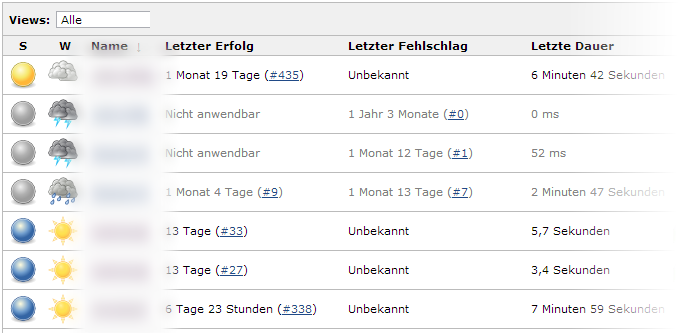
\includegraphics[scale=.45]{Grafiken/jenkins_uebersicht.PNG}}\hspace{3pt}
\fbox{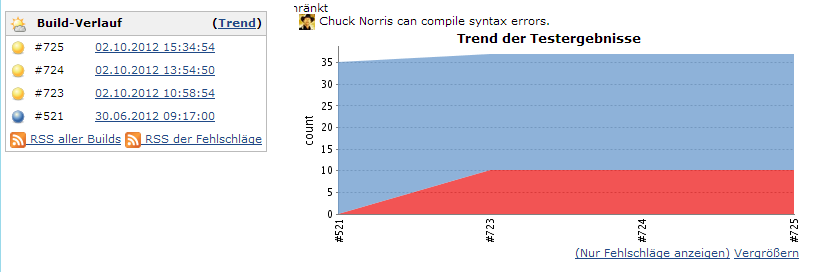
\includegraphics[scale=.45]{Grafiken/jenkins_details.PNG}}
\caption[Jenkins CI-Server - �bersicht]{Jenkins CI-Seve: �bersicht �ber alle Build-Porzesse.}\label{pic:jenkins_all}
\end{figure}

Dieser Prozess ist zentral und kann jederzeit repliziert werden. Hierdurch k�nnen Probleme ausgeschlossen werden, die entstehen, wenn ein derartig gestalteter Prozess auf einem Entwicklersystem durchgef�hrt wird. Die Umgebung, in der ein Entwickler seinen Quellcode erstellt, kann nicht als stabil und verl�sslich angesehen werden. Ein solches System unterliegt zu hohen Seiteneinfl�ssen durch andere Programme und Systeme, als dass ein verl�sslicher und wiederholbarer Prozess m�glich w�re. Die Verl�sslichkeit sowie die Kontrolle �ber m�gliche Seiteneinfl�sse wird jedoch f�r den Build-Prozess vorausgesetzt. Standards, auf die sich verst�ndigt wurde, k�nnen so m�glicherweise nicht eingehalten werden. Scheitert der Prozess, lassen sich aufgetretene Fehler so nicht vollst�ndig replizieren und die Ursache nicht ohne einen Restzweifel ergr�nden. Das vorhandene CI-System ist ein wesentlicher Baustein, solche Fehler zu vermeiden.\footnote{Vgl. \cite{cd_maturitymodel}}

%\comment{Negativ-Beispiel f�r Developer-Build aus CI oder CD heraussuchen.}

Alle erstellten Softwarepakete werden mit einer Versionsnummer versehen und in einem zentralen Repository abgelegt. Nachgeschaltete Tests und Prozesse k�nnen so jederzeit auf die unterschiedlichen Versionsst�nde einer Software zur�ckgreifen. Zu keinem Zeitpunkt wird eine einmal erstellte Version ein zweites Mal kompiliert. Dies ist ein wichtiger Punkt, um auftretende Fehler im Prozess jederzeit replizieren zu k�nnen. W�rde ein Paket innerhalb des Prozesses ein zweites Mal erstellt werden, lassen sich die Bedingungen, unter denen die urspr�ngliche Version erstellt wurde, m�glicherweise nicht mehr herstellen. Der Grund f�r das Fehlverhalten, \zb\ bei einem Testdurchlauf, ist dann nur mit h�herem Aufwand zu ermitteln. Es kann nicht ausgeschlossen werden, dass der Build-Prozess durch eine ver�nderte Konfiguration selbst den Fehler verursacht hat. Wird ein Paket hingegen nur einmal erstellt und kommt es in einem sp�teren Test zu einem Fehlverhalten, l�sst sich die Fehlerursache auf die letzte �nderung der Quellcodebasis zur�ckf�hren. Eine Untersuchung sollte dann den Grund des Fehlverhaltens schnell eingrenzen k�nnen.

Das Management von Abh�ngigkeiten, in Bezug auf 3rd-Party-Bibliotheken, wird in Verbindung mit Maven durch den Nexus Repositroy-Sever unterst�tzt. Der Nexus-Server stellt ein zentrales Repository f�r alle ben�tigten 3rd-Party-Bibliotheken bereit, die in entwickelter Software zum Einsatz kommen. Zudem lassen sich auch die selbst entwickelten Komponenten f�r beliebige andere Prozesse bereitstellen.\footnote{Vgl. \cite{nexus_book}}

Alle Prozesse im Jenkins CI-Server werden automatisch ausgel�st. �bermittelt ein Entwickler seine �nderungen an den bei adesso genutzten Subversion-Server, startet der Jenkins-Server den Build-Prozess. Der Jenkins-Server vergleicht dann die aktuelle Revisionsnummer der Versionsverwaltung mit der zuletzt bekannten und f�r das letzte Build genutzten Revisionsnummer.

Der Jenkins CI-Server ist ein wichtiger Baustein f�r die Realisierung \ci . Er steht jedem Projektteam bereit, welches Technologien verwendet, die durch den Jenkins abgedeckt werden k�nnen. Ob dieses Angebot angenommen werden kann, ist von den Bedingungen abh�ngig, die der Auftraggeber bestimmt. Damit obliegt die genaue Ausgestaltung der \comstage\ den einzelnen Projektteams in Abstimmung mit den speziellen Projektvorgaben.

%Bei kleineren Projekten ist der Aufwand, das Projekte auf die CI-Umgebung vorzubereiten und einheitliche Build-Skripte zu entwerfen, vergleichsweise hoch. Jedoch sind die Schritte die auf der CI-Umgebung durchgef�hrt werden auch in manuellen Schritten auf den Entwicklersystem notwendig.

\subsection{Qualit�tssicherung und \acstage}

Innerhalb der \acstage\ sind die Verfahren zusammengefasst, die sicherstellen, dass eine spezifische Softwareversion den funktionalen sowie nicht-funktionalen Anforderungen gen�gt. Da sich diese Phase durch den Fragebogen nicht vollst�ndig von den Komponenten- und Integrationstests trennen l�sst, werden hier alle Elemente der Qualit�tssicherung ber�cksichtigt.

% --->
In adesso-Projekten wird generell eine hohe Testabdeckung angestrebt, ein Grad von 100\% jedoch nicht vorausgesetzt. Automatisierte Tests werden zum Teil durch manuelle erg�nzt, um die Anwendung hinsichtlich bestimmter Risikoszenarien untersuchen zu k�nnen.

\begin{figure}
\centering
\fbox{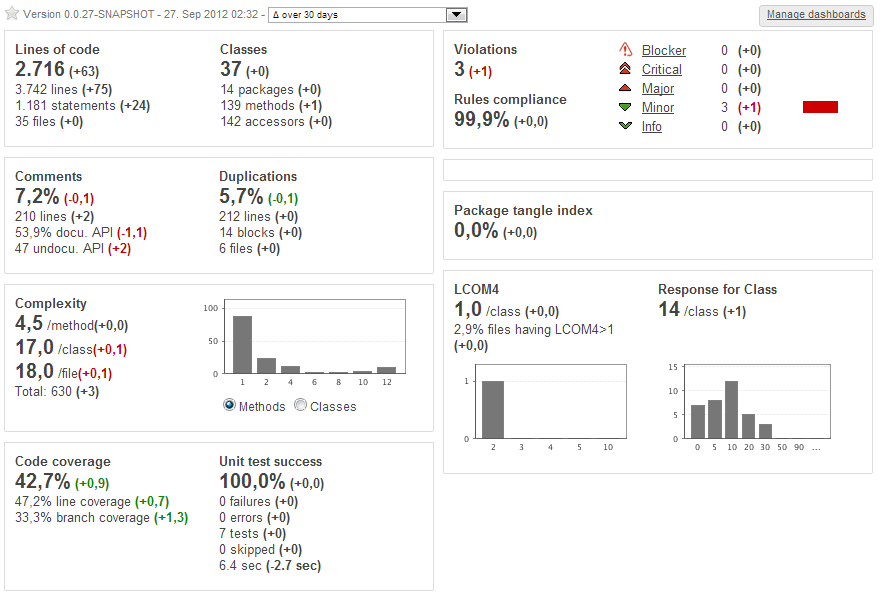
\includegraphics[scale=.5]{Grafiken/sonar_detail.PNG}}
\caption[Detailansicht im Sonar-Server]{Detailansicht eines Projektes im Sonar-Server.}\label{pic:sonar_detail}
\end{figure}

Zur statischen Analyse des Quellcodes wird Sonar, eine Plattform um Code-Qualit�t zu managen, eingesetzt. Sonar bietet die M�glichkeit, Quellcode nach so genanten Coding-Rules zu analysieren. Hierzu geh�ren Namenskonventionen, bekannte Anti-Pattern und Metriken wie die Testabdeckung oder die zyklomatische Komplexit�t von Paketen.\footnote{Vgl. \cite{sonar_features}}

Abbildung~\ref{pic:sonar_detail} zeigt die Detailansicht der statischen Code-Analyse eines Projektes. Relevant ist hier die Einhaltung der vereinbarten Regeln, die dieses Projekt mit $99,9\%$ erf�llt. Zudem k�nnen Ver�nderungen zu vorhergehenden Analysen angezeigt werden.

Weitere Werkzeuge zur statischen Code-Analyse sind:
\begin{itemize}
\item FindBugs\footnote{Weitere Informationen zu FindBugs unter: \url{http://findbugs.sourceforge.net/}},
\item PMD\footnote{Weitere Informationen zu PMD unter:\url{http://pmd.sourceforge.net/}},
\item JaCoCo\footnote{Weitere Informationen zu JaCoCo unter: \url{http://www.eclemma.org/jacoco/trunk/index.html}} und
\item Cobertura\footnote{Weitere Informationen zu Cobertura unter:\url{http://cobertura.sourceforge.net/}}.
\end{itemize}

Neben den Komponenten-Tests und der statischen Analyse des Quellcodes werden breitere Testverfahren auf das Gesamtsystem ausgef�hrt. Ziel dieser Phase ist, das vollst�ndig integrierte System auf die Erf�llung von funktionalen und nicht-funktionalen Anforderungen zu pr�fen.

Automatisierte Akzeptanztests stellen eine M�glichkeit dar, dem Entwicklungsteam eine schnelle R�ckmeldung zu geben, welche Anforderungen vom aktuellen System erf�llt werden. Auch f�r adesso-Projekte sind diese deshalb eine wichtige Grundlage im Entwicklungsprozess und heben den Vorteil des CI-Systems hervor.\footnote{Vgl. \cite[S. 86-87]{CD} und \cite[S. 15]{Duvall07}}

Werden �nderungen der Quellcode-Basis an das Subversion-System �bermittelt, wird die komplette Anwendung kompiliert und die damit verbundenen Tests ausgef�hrt. Dass jede �nderung zum Durchlauf aller Teststufen f�hrt, sichert die Qualit�t zus�tzlich durch Regressionstests. Wirkt sich ein neues Feature negativ auf die Gesamtqualit�t der Anwendung aus, wird dies durch die fortlaufende Qualit�tssicherung entdeckt.\footnote{Vgl. \cite[S. 87]{CD}}

%Aus den Testberichten, die bei jedem Durchlauf erstellt werden, l�sst sich erkennen, welche Test fehlgeschlagen sind und welche erfolgreich waren. Auf diese Weise 

\subsection{Deployment}

Mit dem Deplyoment wird die Software in eine bestimmte Umgebung ausgeliefert. Dabei kann die Zielumgebung des Deployments eine f�r Testzwecke bestimmte Umgebung oder die Produktivumgebung sein. Sind \comstage\ und \acstage richtig angelegt, wird nach jeder �nderung der Quellcodebasis eine neue Instanz des Softwarelieferprozesses erzeugt, an deren Ende eine reife Software f�r den Produktivbetrieb steht. Um die erstellte und gepr�fte Software auch in einem automatisierten Prozess in Produktion zu bringen, erfordert es einige Vorbereitung und kann durch weitere Werkzeuge wie Chef unterst�tzt werden. F�r den bei adesso verwendeten Jenkins CI-Server gibt es die M�glichkeit, ein Deployment auf eine laufende Serverinstanz durchzuf�hren. So kann der Jenkins Deployment-Task \zb\ eine laufende Tomcat- oder JBoss-Instanz ansprechen und mittels Ant-Tasks oder Maven-Goals ein War-File in diese deployen.

Ein komplexeres Deployment, wie z.B. die Auslieferung in eine Infrastruktur, die gegebenenfalls erst installiert und gestartet werden muss, ist nur �ber eigene Skripte m�glich. Hierf�r lassen sich \zb\ Shell- oder Ant-Skripte hinterlegen, die derartige Aufgaben und Werkzeuge ansto�en. Zum Teil ist es aber auch �blich, die ben�tigte Systemumgebung manuell zu konfigurieren und zu installieren. In einigen Projekten konnten auch schon automatische Verfahren in Zusammenhang mit Cloud-Infrastrukturen eingerichtet werden. Das hierbei eingesetzt Werkzeug Chef\footnote{Weitere Informationen zu Opscode Chef unter \url{http://www.opscode.com/chef/}} erm�glicht die Anpassung der Softwarekonfiguration von entfernten Systemen.

%\section{Bewertung nach dem Maturity-Model}

\section{Ankn�pfungspunkte f�r \cd}

Der Prozess, die Anwendung zu kompilieren und zu testen, sollte f�r alle Projekte, bei denen die Bedingungen bestimmt bzw. angeboten werden k�nnen, standardisiert und verpflichtend sein. Manuelle, nicht standardisierte Prozesse, bieten den Entwicklern zwar Flexibilit�t und Individualit�t, erh�hen aber das Risiko, Fehler und Schwachstellen beim Zusammenspiel der unterschiedlichen Softwareteile erst viel zu sp�t zu erkennen. M�glicherweise ist dieser Moment erst kurz vor der geplanten Abnahme der Software durch den Kunden. Dies kann dann zu einer Reihe kurzfristig und nicht ausreichend gepr�fter �nderungen an der Anwendung f�hren. Ein standardisierter Prozess, der bei jeder �nderung auf die gleiche Art und Weise ausgef�hrt wird, hilft ein Fehlverhalten der Anwendung einzugrenzen.\footnote{Vgl. \cite[S. 29-33]{Duvall07}}

In Projekten, bei denen adesso als Lieferant von War- bzw. Ear-Files auftritt, ist ein direktes Deployment in die Produktivumgebung, z.B. durch Sicherheitsrichtlinien des Rechenzentrumsbetreibers, nicht m�glich. Eine voll automatisierte \dpipe\ w�re in diesen F�llen nicht m�glich. F�r die Sicherstellung der Qualit�t sollte der interne CI-Prozess verwendet werden und die Software nach jeder �nderung in eine an das Produktivsystem angelehnte Umgebung installiert und getestet werden.

Projekte mit einem agilen Vorgehen setzen in jeder Iteration neue Funktionalit�ten um. Auf der Seite des Kunden kann es w�nschenswert sein, ein dringend ben�tigtes Feature schnellstm�glich produktiv einsetzen zu k�nnen. Gerade bei Softwaresystemen, bei denen sich auf die Wartung des Systems oder eine kontinuierliche Weiterentwicklung verst�ndigt wurde, kann das automatisierte Deployment einer gut getesteten Software die Kundenzufriedenheit erh�hen und den Prozess in Summe verbessern.

Das Einrichten von Infrastrukturen und Systemen sollte dabei m�glichst nach standardisierten Prozessen ablaufen. Die Schritte f�r Projekte mit einem gleichen Technologie-Stack �hneln sich. Das CI-Team deckt mit seinem Angebot und dem Jenkins CI-Server schon einen gro�en Teil der notwendigen Prozesse f�r \cd\ ab. Hinsichtlich des Deployments k�nnte aber eine vorkonfigurierte \emph{Tool-Chain} den Konfigurationsaufwand f�r neue Projekte deutlich reduzieren. adesso k�nnte so in die F�higkeit versetzt werden, seinen Kunden eine \dpipe\ bei bestimmten Projekten mit anbieten zu k�nnen. Die Untersuchung der drei Werkzeuge wird weiteren Aufschluss �ber die m�glichen Ansatzpunkte f�r \cd\ bieten.

%\comment{Bei adesso werden Systeme wie Jenkins f�r CI und Chef f�r den automatisierten Aufbau einer Infrastruktur bereits eingesetzt. Das sollte zumindest erw�hnt werden um dann konkrete Vorschl�ge f�r andere Tools zu machen, die sich hier eventuell integrieren lassen. K�nnte auch sein, dass hier ein Widerspruch mit der derzeitigen Infrastruktur entsteht und kein Tool sich nahtlos integrieren l�sst. Z.B. kann das der Fall beim CI-Server sein.}

\comment{Es sollen drei Werkzeuge untersucht werden (Thoughtworks Go, Deployinator von Etsy und Dreadnot von Rackspace), die \cd\ ma�geblich unterst�tzen k�nnen. Was leisten diese im Hinblick auf \cd ? Hier ist ein Evaluierungsbogen notwendig, um die Werkzeuge dahingehend untersuchen zu k�nnen, in wie weit diese \cd\ unterst�tzen und f�r einen Einsatz bei adesso geeignet w�ren. Die Untersuchung des Entwicklungsstandes bei adesso ist hierf�r eine Voraussetzung, um zu verstehen welche Technologien derzeit eingesetzt werden und welche Werkzeuge sich in die bestehende Landschaft am besten integrieren lassen. Die Evaluierung der Werkzeuge kann eine Testinstallation erforderlich machen, in dem eine kleines Web-Testprojekt durch eine Deployment Pipeline schickt.}

\chapter{Werkzeuge f�r \cd}

Als Ziel dieser Arbeit wurde die Evaluierung von drei Werkzeugen, die adesso f�r die Umsetzung von \cd\ als interessant eingestuft hat, gesetzt. Dabei m�chte adesso vornehmlich herausfinden, wie diese Werkzeuge funktionieren und aufgebaut sind und wie sich damit eine \dpipe\ umsetzen l�sst. Vor einer genaueren Untersuchung der Eigenschaften ist eine Grobbetrachtung sowie eine Aufstellung von Beurteilungskriterien notwendig. Im Anschluss daran werden die Werkzeuge auf einer Testumgebung installiert und k�nnen dann genauer nach ihren Funktionalit�ten untersucht werden. 

An \cd\ und den M�glichkeiten einer \dpipe\ besteht bei adesso ein hohes Interesse. Mit dem Jenkins-Server wird bereits ein System f�r \ci\ verwendet und damit der erste Teil von \cd\ verwirklicht. Untersucht werden soll Go von Thoughtworks, Deployinator von Etsy und Dreadnot von Rackspace. Mit der Evaluierung von Go, Deployinator und Dreadnot m�chte adesso herausfinden, ob ein L�ckenschluss zwischen dem CI-System und der Verwaltung von Infrastrukturen mit Werkzeugen wie Chef m�glich ist.

\section{Kriterien f�r die Evaluierung}

F�r die Evaluierung der Werkzeuge ist kein spezielles Anwendungsszenario vorgegeben, wie \zb\ f�r ein bestimmtes Projekt eine \dpipe\ mit Hilfe eines dieser Werkzeuge umzusetzen. Aus diesem Grund werden die F�higkeiten der Werkzeuge nach allgemeinen Kriterien betrachtet und der Rahmen ber�cksichtigt, in dem sich die adesso Projekte aus dem Umfeld der Web-Technologien bewegen.

adesso sieht in \cd , in Zusammenhang mit Cloud-Techniken, eine m�gliche zuk�nftige Ausrichtung, auf deren Basis sich neuartige Dienstleistungen errichten lassen. Im Zentrum steht hier nicht die Auswahl einer geeigneten Software mit anschlie�ender Einf�hrung, sondern viel mehr eine Betrachtung der sich bietenden Optionen f�r zuk�nftige Projekte und Dienstleistungen.

Der genaue Funktionsumfang dieser Werkzeuge als auch die verfolgten Ans�tze sind vorerst nicht weiter bekannt. Implikationen f�r ein Liefersystem ergeben sich aber aus Abschnitt~\ref{konzepte_cd} und \ref{liefersystem} und wurden unter Punkt~\ref{lierfsys_implikation} zusammengefasst. Kriterien f�r eine Evaluierung k�nnen hieraus abgeleitet werden.

\subsection{Einordnung der Werkzeuge}

Eine einf�hrende Grobbetrachtung der zu untersuchenden Werkzeuge zeigt, dass sich die Werkzeuge in unterschiedlichen Klassen befinden und nicht dieselben Ziele verfolgen.

Bei \go\ handelt es sich um ein vollwertiges CI-System in dem die Phasen der \dpipe\ abgebildet werden k�nnen. \dr\ und \dpl\ sind vornehmlich Self-Service-Portale, die das Deployment ansto�en sollen.

Ein direkter Vergleich der Werkzeuge wird nicht m�glich sein, da der Funktionsumfang zu unterschiedlich ist, um eine objektive Beurteilung zu erm�glichen. F�r eine unabh�ngige Betrachtung der Werkzeuge spricht auch die Implikation, f�r neue Dienstleistungen und zuk�nftige Projekte unterschiedliche Ans�tze ableiten zu k�nnen. 

Die unabh�ngige Betrachtung schlie�t aber nicht einen Vergleich von allgemeinen Qualit�tsmerkmalen von Software aus sowie die Untersuchung, welche Merkmale einer \dpipe\ konkret abgebildet werden k�nnen. F�r den derzeitigen Lieferprozess w�re es eine Verbesserung, wenn die automatisierte Auslieferung von Software in die Test- und Produktivumgebung sich �ber ein Portal besser organisieren lassen w�rde. 

In einem Kunden-Lieferanten-Verh�ltnis ist ein direktes Liefern in die Produktivumgebung h�ufig aus vertragsrechtlichen Einschr�nkungen oder Gr�nden der Compliance nicht m�glich. adesso als Dienstleister f�r individuelle Softwarel�sungen k�nnte in diesem Fall aber ein \ssp\ als zus�tzliche Dienstleistung bereitstellen, in das sich Mitarbeiter des Kunden einloggen k�nnen. Die Testabteilung des Kunden oder der IT-Betrieb dann das Deployment der gew�nschten Version ansto�en.

\subsection{Allgemeine Kriterien}

Die Qualit�t von Software l�sst sich durch die definierte Qualit�tscharakteristika der DIN/ISO-9126 beschreiben. Durch diese Kriterien l�sst sich eine Software nach Funktionalit�t, Zuverl�ssigkeit, Benutzbarkeit, Effizienz, Wartbarkeit und Portabilit�t beurteilen.\footnote{Vgl. \cite[S. 57f]{starke_swa} und \cite[S. 110]{balzert_swt}} Diese Kriterien sollen auch f�r einen allgemeinen Vergleich von \go , \dpl\ und \dr\ genutzt werden, um eine vergleichende Aussage der Werkzeuge zu erm�glichen.

\paragraph{Funktionalit�t}

Mit der Funktionalit�t wird das Vorhandensein von Funktionen einer Anwendung mit festgelegen Eigenschaften und die angemessene Erf�llung der Anforderungen beschrieben. In Bezug auf die Konzepte von \cd\ bedeutet dies die M�glichkeit, eine \dpipe\ abbilden zu k�nnen und die Unterst�tzung einer weitgehenden Automatisierung der dazugeh�rigen Prozesse. Die Anforderungen leiten sich aus \cd\ ab.

Damit die Anwendung mit den vorgegebenen Systemen zusammenarbeiten kann, muss gepr�ft werden, wie weit die Anwendung sich in die bestehende Systemlandschaft integrieren l�sst. F�r adesso ist es erforderlich, dass die betrachtete Anwendung mit dem bestehenden CI-System zusammenarbeitet.

\paragraph{Zuverl�ssigkeit}

Mit der Zuverl�ssigkeit wird die Reife des Produktes zum Ausdruck gebracht. Dabei spielen folgende Faktoren eine Rolle:

\begin{itemize}
\item Eine geringe Versagensh�ufigkeit,
\item die Reaktion des Systems auf Fehlerzust�nde und 
\item die M�glichkeit den Zustand des Systems nach einem Versagen wiederherstellen zu k�nnen.
\end{itemize}

Eine Aussage �ber die Reife kann \zb\ das Entwicklungsstadium der Anwendung sein. Mit einer Versionsnummer kleiner $1.0$ wird signalisiert, dass es sich noch um keine f�r ein Release freigegebene Version der Software handelt. Zum Vergleich von Reife zwischen Anwendungen ist dies allerdings kein Kriterium.

\paragraph{Benutzbarkeit}

Die Benutzbarkeit einer Anwendung kann �ber ihre Verst�ndlichkeit, Erlernbarkeit und Bedienbarkeit beurteilt werden. Bei einer verst�ndlichen Anwendung muss ersichtlich sein, welche Funktionen welche Zust�nde und Prozesse ansto�en. Der Aufwand, das Konzept der Anwendung zu verstehen, muss gering sein. Zudem muss der Einstieg in die Anwendung leicht und schnell erlernbar sein. Konfiguration und Bedienung sollen leicht sein und in verst�ndlichen Schritten erfolgen.

\paragraph{Effizienz}

Mit der Effizienz wird das Zeitverhalten einer Anwendung untersucht. Die Anwendung sollte schnell auf Nutzereingaben reagieren k�nnen und die Antwortzeit bei einer Funktionsausf�hrung gering sein. Weiterhin wird hier das Verbrauchsverhalten in Form der ben�tigten Betriebsmittel untersucht, die das System f�r den Betrieb ben�tigt. Als Vergleichsma�stab k�nnen die angegebenen Systemvoraussetzungen herangezogen werdend.

\paragraph{Wartbarkeit und �nderbarkeit}

Der Aufwand, M�ngel der Anwendung sowie deren Ursache zu finden, sollte gering sein. Sind Anpassungen der Anwendung notwendig, stellt sich die Frage nach den Voraussetzungen, um eine Anpassung durchf�hren zu k�nnen sowie der damit verbundene Aufwand.

\paragraph{Portabilit�t und �bertragbarkeit}

Die Anpassbarkeit beschreibt die M�glichkeit, die Anwendung an eine andere Umgebung anzupassen. Demnach sollte das System auf unterschiedlichen Plattformen und Systemkonfigurationen ausgef�hrt werden k�nnen.

Zudem steht hier die Durchf�hrung und der Aufwand von Installation und Inbetriebnahme der Anwendung auf dem Pr�fstand. Um eine Anwendung in den Betrieb zu nehmen, muss die Installation gut dokumentiert, verst�ndlich und vollst�ndig sein.

\subsection{Anforderungen f�r \cd}

Aus \cd\ leiten sich Anforderungen ab, die von einer \dpipe\ ber�cksichtigt werden m�ssen. Es wird nicht erwartet, dass es ein Werkzeug gibt, welches alle Anforderungen erf�llt. Vielmehr haben \hf\ bei der Beschreibung der \dpipe\ auf den Einsatz von spezialisierten Werkzeugen und Shell-Skripten verwiesen.

\go , \dpl\ und \dr\ sollen gegen die Anforderungen von \cd\ gepr�ft werden, damit ersichtlich wird, welche Elemente der \dpipe\ abgebildet werden k�nnen und f�r welche ein erg�nzendes Werkzeug gefunden werden muss, um eine vollst�ndige \dpipe\ verwirklichen zu k�nnen.

Nach \hf\ besteht die \dpipe\ aus einzelnen Stages, die parallel oder sequenziell verlaufen k�nnen. F�r die \dpipe\ muss es also M�glichkeiten geben, Prozesse abbilden zu k�nnen. Eine Oberfl�che f�r das Management der \dpipe\ sollte anzeigen, welche Version in welche Umgebung deployt wurde und welche Revisionsnummer der Code-Basis genutzt wurde.

Um den Lieferprozess anzusto�en, muss dieser getriggert werden k�nnen. Dabei sollte der Teil von \ci\ durch eine neue Version der Code-Basis automatisch angesto�en werden, w�hrend es f�r das Deployment auf das Test- und Produktivsystem automatische oder manuelle M�glichkeiten geben sollte. Letzteres m�sste dann �ber eine Oberfl�che zug�nglich sein und \zb\ �ber einen einfachen Knopfdruck angesto�en werden k�nnen.

Weitere Komponente sind die Dokumentation sowie ein schnelles Feedback an den Nutzer. Folgende Elemente sollten dokumentiert und dargestellt werden:

\begin{itemize}
\item Die Durchlaufzeit einer Stage, 
\item die Fehler, die aufgetreten sind sowie deren Gr�nde, 
\item die Anzeige von Test-Reports, die eine qualitative Beurteilung des Builds erm�glichen.
\end{itemize}

Die \comstage\ und \acstage\ erfordern die Kommunikation und Ausf�hrung verschiedener Systeme und Programme zur Erf�llung der Aufgaben dieser Stage. Hierzu geh�ren das Laden der aktuellen Quellcode-Basis aus der Versionsverwaltung, das Ansto�en von Build-Tool, die Verwaltung der Binaries in einem Repository, die Ausf�hrung von Test-Skripts und die Vorbereitung der Ausf�hrungsumgebung f�r Test und Produktion.
 
Die in diesen Bereichen vorhandene Infrastruktur von adesso muss Ber�cksichtigung finden. So wird f�r die Verwaltung der Quellcode-Basis Subversion (SVN) eingesetzt und je nach Projekt Ant oder Maven zum Erstellen der Binaries verwendet.

\section{Evaluierung der Werkzeuge}

\subsection{\go\ von Thoughtworks}

\go\ wird von ThoughtsWors Studois\footnote{Informationen zu ThoughtWorks Studios unter \url{http://www.thoughtworks-studios.com/} .} entwickelt. Der Fokus von ThougthWorks liegt auf Software, die agile Methoden unterst�tzen. \go\ wird unter dem Slogan \mycite{Agile Release Management} angeboten.\footnote{Vgl. \cite{go_company}}

\subsubsection{Konzept von \go}

Mit \go\ k�nnen automatisierte Build-, Tests und Releaseprozesse modelliert werden. Dabei wird das Konzept eines \mycite{push-button deployments} unterst�tzt. Das Konzept von \go\ baut auf \ci\ auf und erweitert dieses um Funktionen f�r \cd . Dabei k�nnen verschiedene Pipelines f�r verschiedene Projekte und Produkte mit unterschiedlichen Nutzerkreisen verwaltet werden. \go\ kann Pipelines parallel verarbeiten, in dem es ein Netz von verteilten Agents nutzt.

In einer Pipeline k�nnen verschiedene Stages angelegt werden, die dann nacheinander abgearbeitet werden. Jede Stage kann einen oder mehrere Jobs definieren. Dabei dienen die Jobs der B�ndelung von Tasks. Die Jobs einer Stage werden parallel ausgef�hrt und auf freie Agents verteilt. Die in einem Job gegliederten Tasks werden dann aber sequenziell abgearbeitet.

\go\ ist eine auf den Jetty-Server\footnote{Der Jetty Server ist seit 2009 ein Teil der Eclipse Foundation. Weitere Informationen unter \url{http://www.eclipse.org/jetty/about.php} .} basierende Web-Applikation, welche diesen in den Anwendungskern einbettet. Die Ausf�hrung einer Stage wird von verteilt oder lokal laufenden Agents durchgef�hrt, die sich mit dem go-Server verbinden.

\subsubsection{Lizenzvarianten}

\go\ wird in drei Preisvarianten angeboten, eine kostenfreie Community- und zwei propriet�re Enterprise-Versionen. Der wesentliche Unterschied zwischen den Varianten besteht in der Anzahl der erlaubten User und der verteilt laufenden Agents. Agents, die lokal auf dem System des \go -Server ausgef�hrt werden, k�nnen je nach vorhandener Kapazit�t der Hardware unbegrenzt gestartet werden.

\begin{figure}
\centering
\fbox{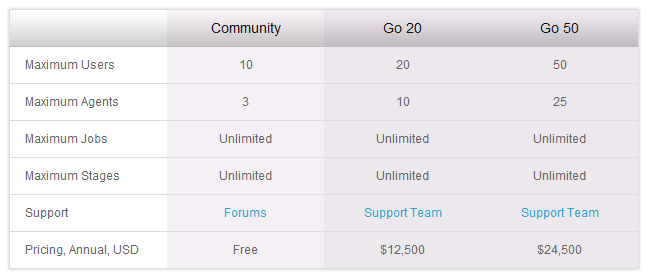
\includegraphics[scale=0.8]{Grafiken/go_pricing.PNG}}
\caption[Version und Preise von \go]{Versionen und Preise von \go , Quelle: \cite{go_pricing}.}\label{pic:go_pricing}
\end{figure}

Abbildung~\ref{pic:go_pricing} zeigt die Unterschiede zwischen den Versionen Community und der Enterprise. Bis einschlie�lich zur Version $12.2$ war es mit der kostenfreien Community-Version nicht m�glich, ein Cluster mit Agents zu betreiben. Zul�ssig waren bis dahin nur Agents, die auf der Server-Instanz ausgef�hrt worden sind. Mit Version $12.3$ k�nnen in der Community-Version auch bis zu drei verteilt laufende Agents im Go-Server angemeldet werden. In der Enterprise-Version k�nnen bis zu 10 oder 25 verteilt laufende Agents betrieben werden. Zudem bietet Thoughtworks hier ein unterst�tzendes Support-Team, welches bei der Konfiguration des Systems helfen kann.\footnote{Vgl. \cite{go_pricing}}

\subsubsection{Testprojekt und Probeversion}

\hf\ empfehlen f�r die Umsetzung einer \dpipe\ am Anfang ein funktionierendes Skelett der geplanten Anwendung zu verwenden.\footnote{Vgl.  \cite[S. 132]{CD}} Thoughtworks hat f�r die Erprobung eine Test-Lizenz f�r 30 Tage bereitgestellt, mit der sich die Vorteile der Enterpriseversion nutzen lassen.

F�r den Probebetrieb von \go\ muss eine Netzwerkinfrastruktur mit mehreren Servern simuliert werden. Dies ist dadurch begr�ndet, dass \go\ Funktionalit�ten von \ci\ bietet und Subsysteme wie Versionsverwaltung und Testserver f�r einen f�r den Probebetrieb ben�tigt werden sowie selbst als Server-Agent-Architektur realisiert wurde.

Ausgangspunkt der \dpipe\ ist das Entwicklersystem. Dieser �bermittelt seine �nderungen am Quellcode in das Versionsverwaltungssystem. Hierf�r wird die Eclipse IDE genutzt und eine einfache Hello-World-Applikation, mit dem Projekt-Wizzard von Eclipse, als dynamisches Web-Projekt angelegt. Ziel des Testprojektes ist die Untersuchung der Konfigurationsf�higkeit und der Funktionalit�t von \go . Strukturell betrachtet wird \go\ verteilt ausgef�hrt. Dabei verbinden sich Agents mit dem Server und teilen ihren Status mit. Der Server verteilt neue Auftr�ge an freie Agents.

Um einen Test dieser Struktur zu erm�glichen, werden drei virtuelle Systeme mit VirtualBox\footnote{Mehr Informationen zu VirtualBox unter \url{https://www.virtualbox.org/} .} erzeugt und die Server-Variante von Ubuntu ohne GUI darauf installiert. Diese Struktur wird angelegt, um ein verteiltes System zu simulieren. Abbildung~\ref{pic:go_test_aufbau} zeigt die Netzkonfiguration f�r die virtuellen Systeme und den Host. Auf Grund von Kapazit�tsbeschr�nkungen des Host-Systems werden die Test-Umgebung und das Versionsverwaltungssystem zusammengelegt.

\begin{figure}
\centering
\fbox{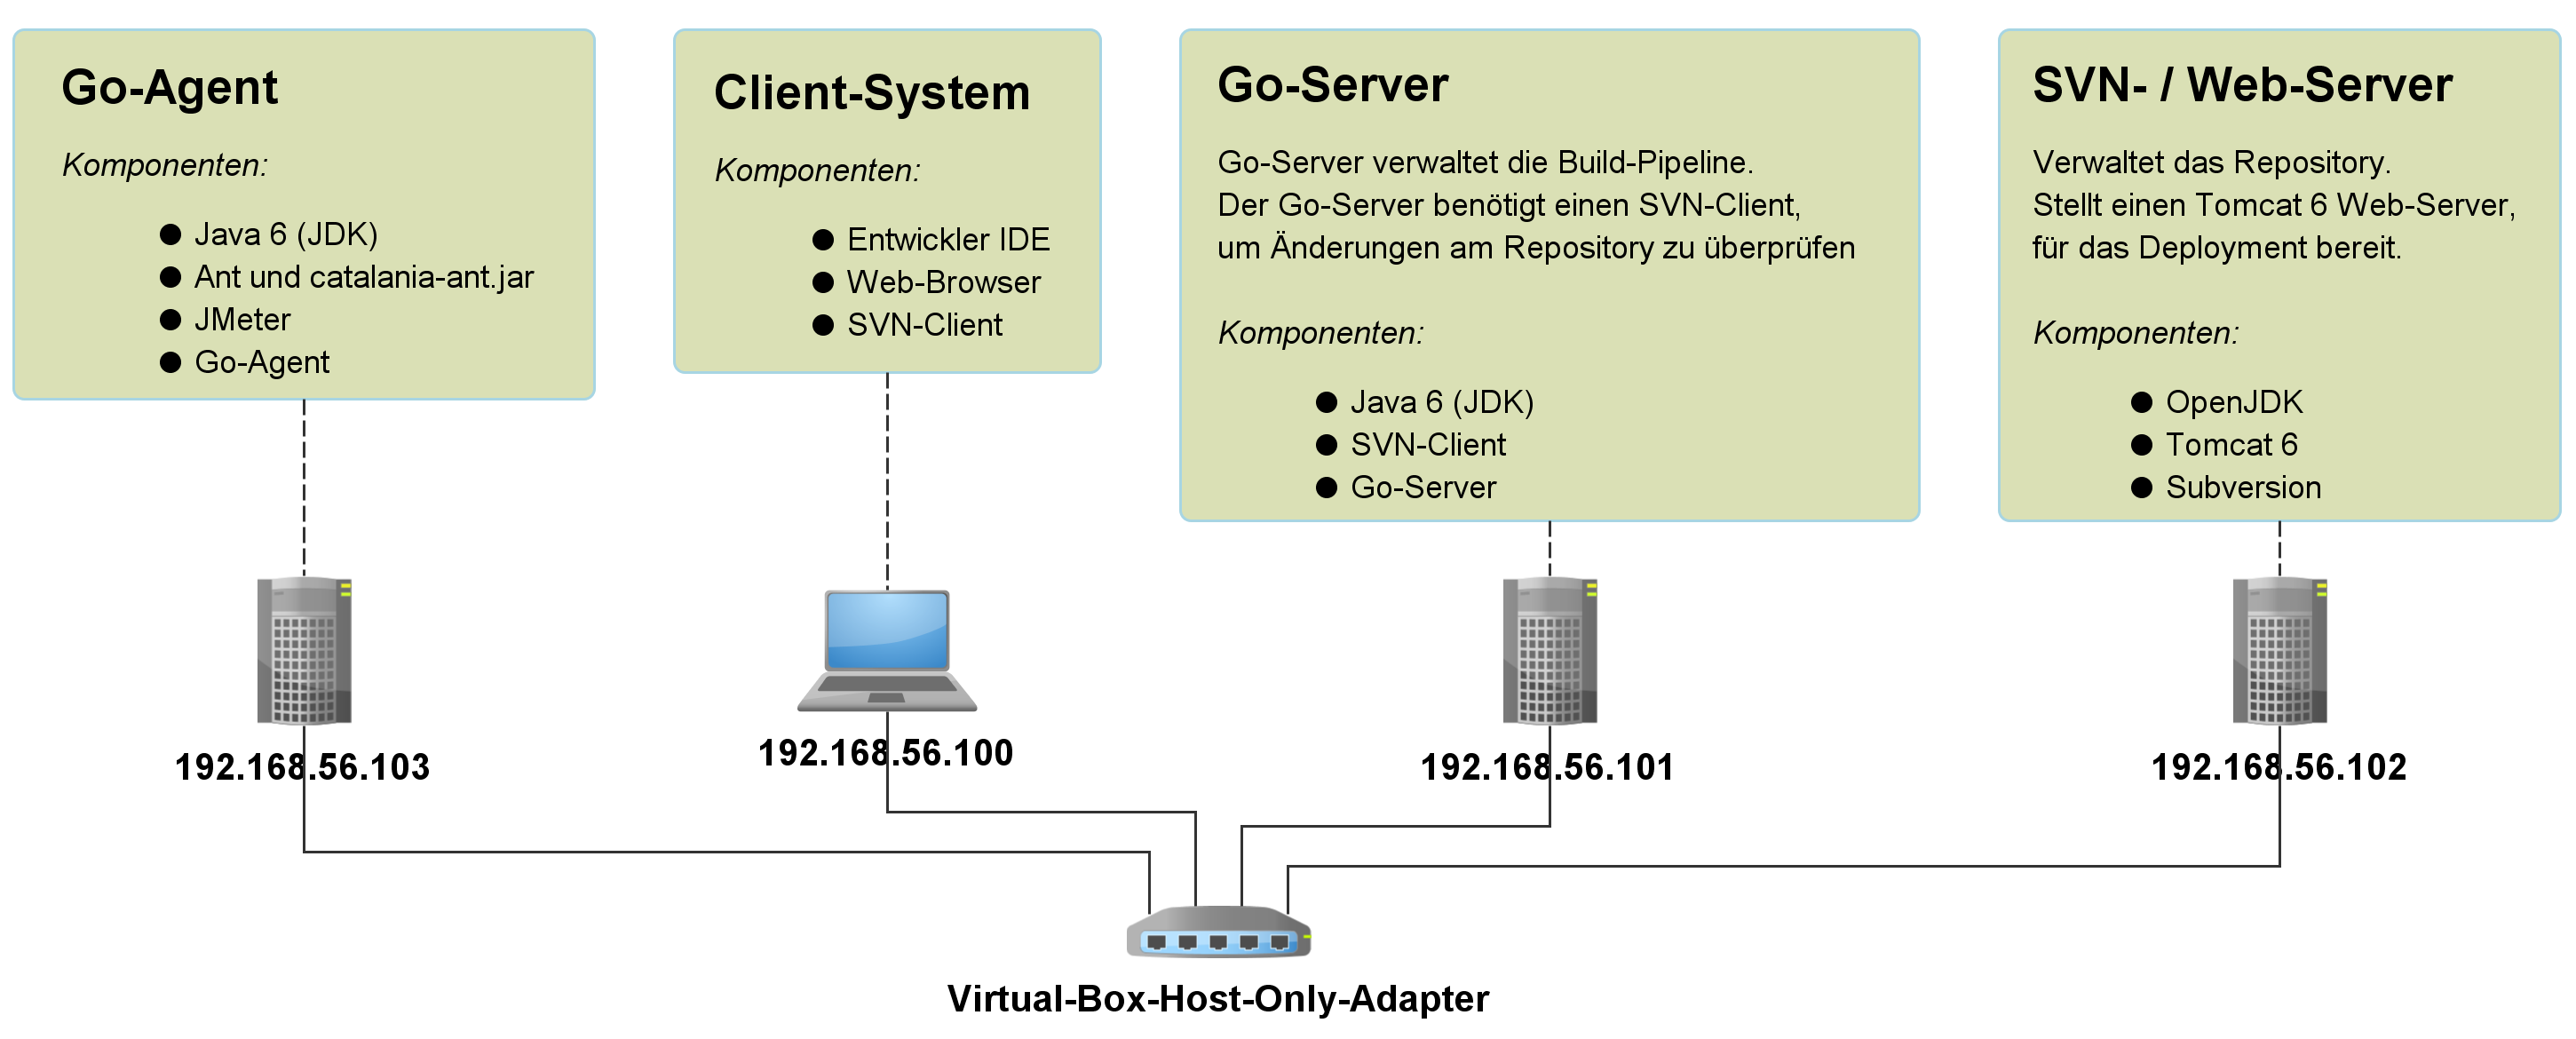
\includegraphics[width=\linewidth]{Grafiken/Test_Konfiguration_Go.PNG}}
\caption[\go -Testaufbau mit VirtualBox]{Testaufbau mit VirtualBox.}\label{pic:go_test_aufbau}
\end{figure}

Auf den virtuellen Systemen wird Ubunut~11.10 f�r 32~Bit Architekturen. Der \go -Server wurde mit 1280~MB Arbeitsspeicher ausgestattet, Systemvoraussetzung sind 1~GB, empfohlen aber 2~GB, die vom Host aber nicht bereitgestellt werden k�nnen. Der \go -Agent ben�tigt weniger Ressourcen und ist mit 256~MB ausgestattet. Gleiches gilt f�r die Test-Umgebung.

%\begin{wrapfigure}{r}{0.33\textwidth}
%\centering
%\fbox{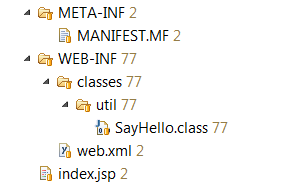
\includegraphics[scale=0.6]{Grafiken/hello_world_projektstruktur.PNG}}
%\caption[Testprojekt]{Struktur des Testprojektes.}\label{fig:test_project}
%\end{wrapfigure}

Auf allen Systemen kommt das Java Development Kit in Version~6 Update~31 f�r 32-Bit-Architekturen zum Einsatz. Zur Zeit der Erprobung war Verison~12.2 aktuell. Die Abarbeitung der Jobs einer Stage wird durch Agents durchgef�hrt. Da Jobs parallele Abl�ufe einer Stage verwirklichen, k�nnen Jobs einer aktiven Stage auf verschiedene Agents verteilt werden. F�r die Umsetzung der in Tasks vorgesehenen Aufgaben m�ssen auf dem Agent-System alle Voraussetzungen geschaffen werden. Der Build-Prozess des Testprojektes basiert auf Ant und JUnit-Tests f�r die Komponenten, was eine Installation von Ant und JUnit notwendig werden l�sst. Die Quellcode-Basis muss auf das System geladen werden, wof�r Subversion genutzt und ein SVN-Client installiert wird. Im weiteren Verlauf werden Akzeptanz- und Kapazit�tstests mit Hilfe von Apache JMeter und JWebUnit durchgef�hrt. Die hierf�r ben�tigen Bibliotheken m�ssen auf dem Agent-System vorhanden sein. Die Testumgebung wird auch f�r die Verwaltung der Code-Basis verwendet, was die Installation von Subversion bedingt. F�r die automatisierten Akzeptanz-Tests wird ein Tomcat-Server in Version~6 als Deploymentziel verwendet.

\begin{figure}
\centering
\fbox{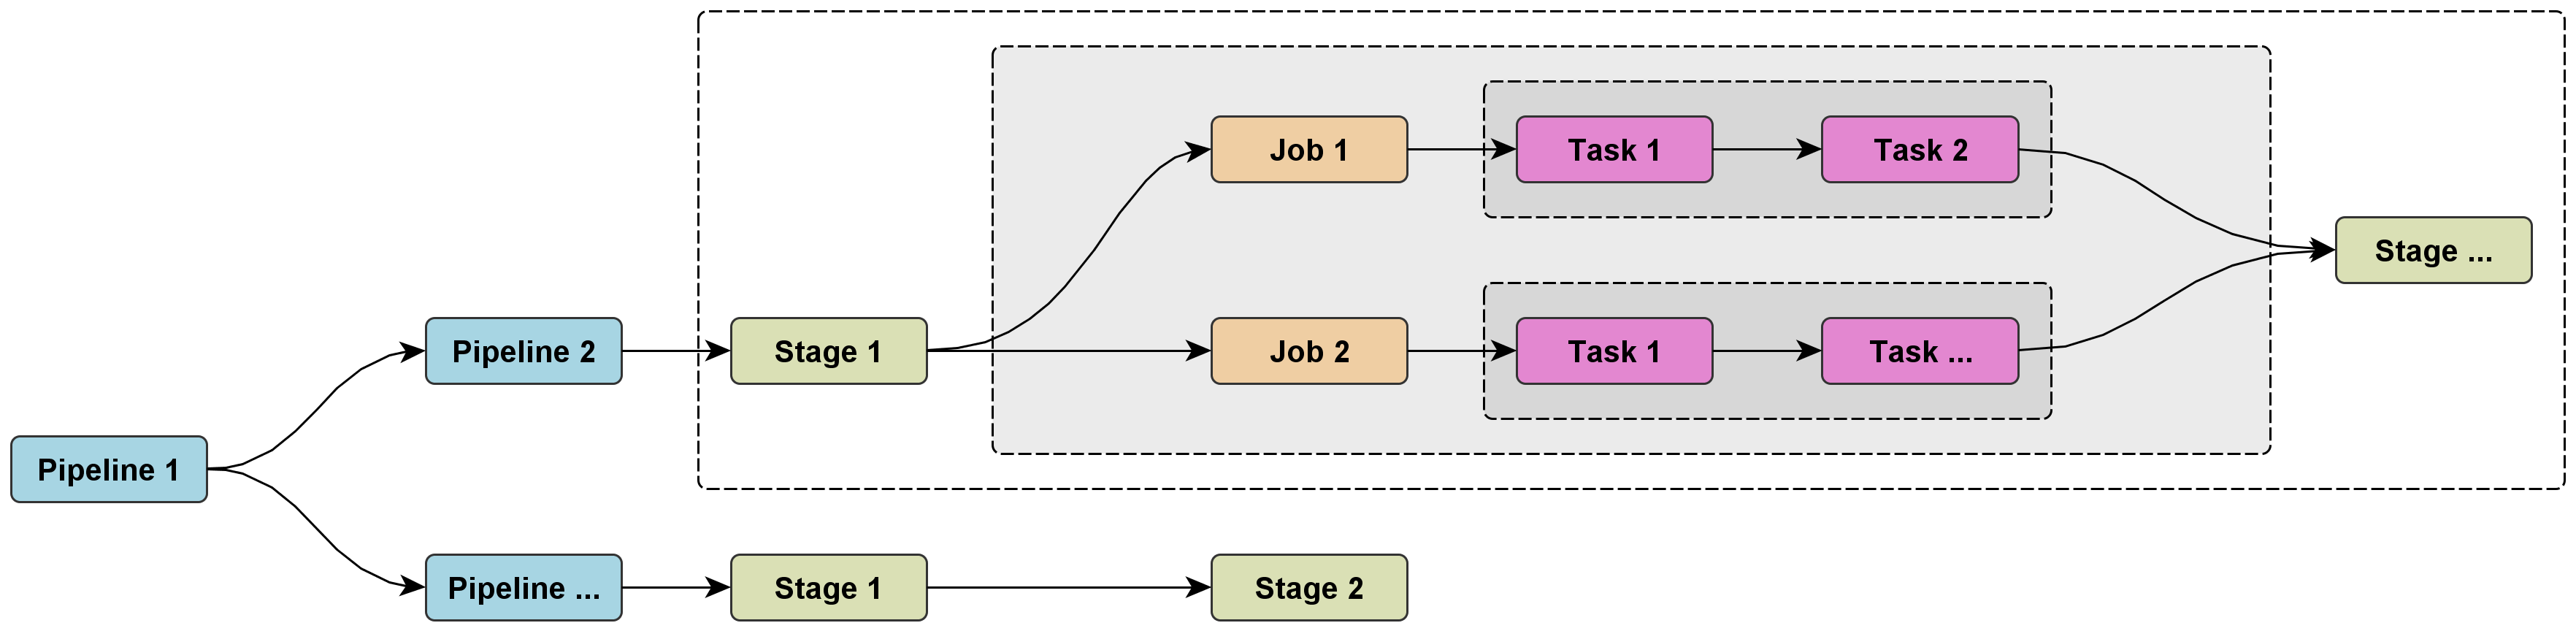
\includegraphics[width=\linewidth]{Grafiken/go_pipeline_und_stages.PNG}}
\caption[Konzept der Pipelines und Stages in \go]{Konzept der Pipelines und Stages in \go .}\label{pic:go_stages_konzept}
\end{figure}

Der Ablauf des Testsystems sieht \comstage\ und \acstage\ vor. F�r die \acstage\ muss die Testanwendung in das Testsystem deployt werden. Die \dpipe\ endet hier f�r das Versuchsprojekt, da alle komplexeren Vorg�nge sich auf gleiche Art und Weise konfigurieren werden und \go\ dabei ausschlie�lich das Ansto�en dieser Aufgaben in Form von Skripten erm�glicht. Komplexere Szenarien k�nnten hier \zb\ mit Hilfe von Werkzeugen wie Chef umgesetzt werden. Infrastructure-As-A-Service, abgek�rzt IaaS, ist ein Ansatz, Rechnerinfrastrukturen bei Bedarf ben�tigter Serverressourcen mieten zu k�nnen, welcher als ein Teil des so bezeichneten Cloud-Compunting verstanden wird.\footnote{Vgl.: \cite{Huth2011}} Ein derartiges Szenario ist aber nicht Gegenstand dieser Arbeit und Werkzeuganalyse, sollte mit anderen Arbeiten aber noch weiterf�hrend betrachtet werden.

\subsubsection{Funktionen}

\paragraph{Pipeline Management}



Eine Pipeline kann in \go , wie es \hf\ empfehlen, durch verschiedene Stages abgebildet werden. Pipelines wiederum k�nnen Ausgangsmaterial f�r andere sein, bzw. selbst durch andere angesto�en werden. Das Konzept von Pipeline, Stages, Jobs und Tasks in \go\ zeigt Abbildung~\ref{pic:go_stages_konzept}. Mehrere Pipelines lassen sich zu einer Baumstruktur verzweigen. Die Stages einer Pipeline werden, je nach Ergebnis der vorhergehenden Pipeline, sequentiell abgearbeitet. In einer Stage werden dann Jobs an freie Agents verteilt. Dieses Konzept erm�glicht die Abarbeitung unterschiedlich lang laufender Akzeptanztests. Dies ist ein Vorgehen, welches \hf\ empfehlen damit Fail-Fast ein fr�hestm�gliches Scheitern der Pipeline bei Fehlern in der Quellcode-Basis erm�glicht wird und ein schnelles Feedback an die Entwickler gegeben werden kann.

\begin{wrapfigure}{r}{0.6\textwidth}
\centering
\fbox{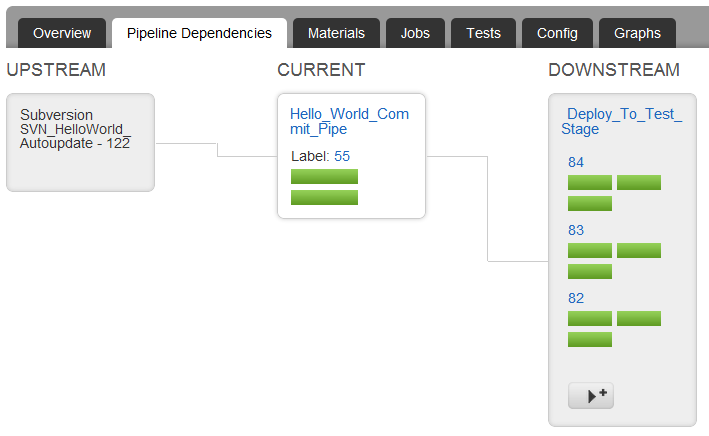
\includegraphics[scale=0.5]{Grafiken/go_003_Pipeline_Run_Dependencies_cut.PNG}}
\caption[Dependencie Graph]{Dependencie-Graph der Pipelines.}\label{pic:go_dependency}
\end{wrapfigure}




Angesto�en werden kann die Pipeline durch verschiedene Trigger. Trigger k�nnen entweder die verwendeten Materialien der Pipeline sein oder ein manuelles Ansto�en �ber die Oberfl�che. Als Materialien werden die Versionsverwaltungssysteme und Pipelines bezeichnet, deren aktueller Stand oder letzte Ergebnisse, Ausgangsmaterial einer Stage sind. Wird \zb\ das Material Subversion verwendet, reagiert das System auf Ver�nderungen der Code-Basis in der Versionsverwaltung von Subversion und erzeuge eine neue Instanz der Pipeline mit der aktuellen Revisionsnummer des Materials. Abbildung~\ref{pic:go_dependency} zeigt die Abh�ngigkeiten f�r die mittlere Pipeline (CI Pipeline) in Zusammenhang mit Up- (Subversion) und Downstream (Deploy-Pipeline).



%\begin{wrapfigure}{r}{0.5\textwidth}
%\centering
%\fbox{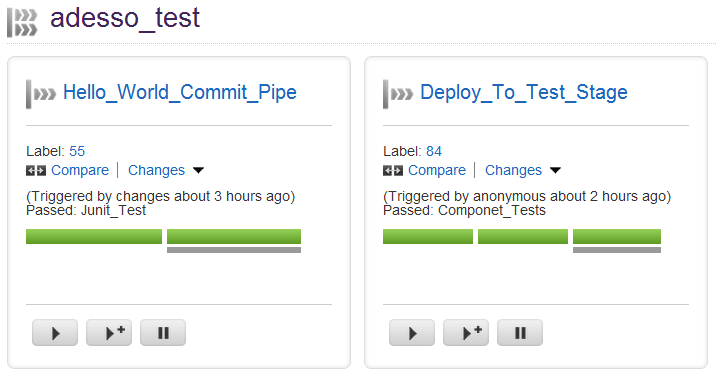
\includegraphics[scale=0.5]{Grafiken/go_001_Pipeline_Main_Window_cut.PNG}}\\
%\vspace{\baselineskip}
%\fbox{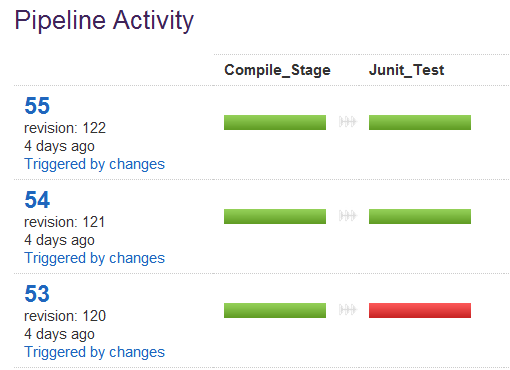
\includegraphics[scale=0.5]{Grafiken/go_002_Pipeline_Activity_cut.PNG}}
%\caption[Pipeline�bersicht und Historie in \go]{�bersicht �ber die Pipelines und deren Historie.}\label{pic:go_pipelines_overview}
%\end{wrapfigure}

Die Oberfl�che von \go\ gibt dem Entwicklungsteam ein schnelles Feedback �ber den Zustand der Quellcode-Basis. Abbildung~\ref{pic:go_pipelines_overview} zeigt die Einstiegsseite sowie die Historie der Instanzen einer Pipeline.

\go\ erzeugt beim Durchlauf eines Tasks Log-Dateien, die �ber die Oberfl�che ausgerufen werden k�nnen. Werden in einem Task Test-Protokolle im HTML-Format erstellt, k�nnen diese in die Oberfl�che eingebunden und angezeigt werden. Abbildung~\ref{pic:go_test_report} zeigt auf der rechten Seite das eingebundene Testprotokoll von JUnit, welches w�hrend eines Durchlaufs erzeugt wurde. Die Log-Datei ist auf der linken Seite zu sehen. Die Log-Datei hilft Fehler im Durchlauf zu identifizieren.

\begin{figure}
\centering
\fbox{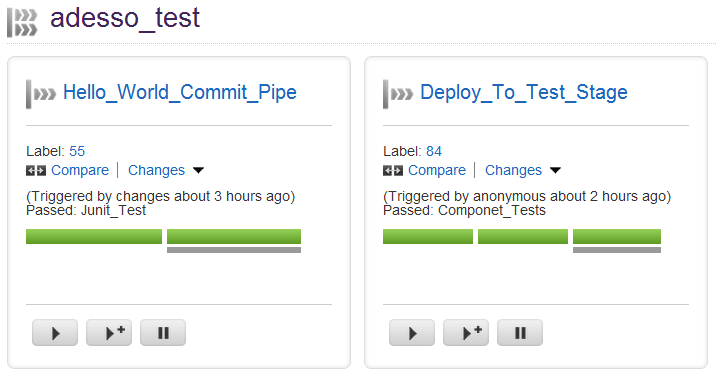
\includegraphics[scale=0.5]{Grafiken/go_001_Pipeline_Main_Window_cut.PNG}}\hfill
\fbox{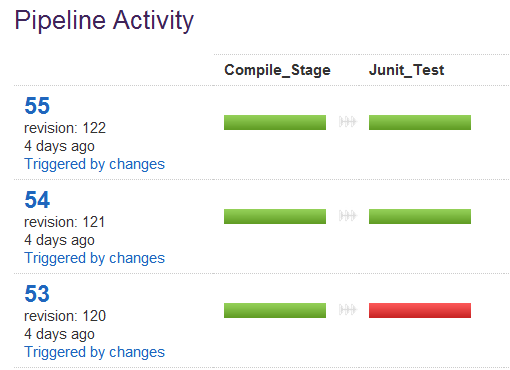
\includegraphics[scale=0.5]{Grafiken/go_002_Pipeline_Activity_cut.PNG}}
\caption[Pipeline�bersicht und Historie in \go]{�bersicht �ber die Pipelines und deren Historie.}\label{pic:go_pipelines_overview}
\end{figure}


\paragraph{Stages}

F�r die \comstage , welche Teil von \ci\ ist, k�nnen die \verskont e von Apache Subversion, Git, Mercurial, Preforce und der Microsoft Team Foundation Server als Materialien genutzt werden. Im Testprojekt wurde Subversion installiert, um die Code-Basis zu verwalten. Das Material gilt f�r die gesamte Pipeline, welche mit der aktuellen Versionsnummer instantiiert wird. Jeder Job beginnt mit dem Laden der aktuellen Version der Code-Basis in das lokale Verzeichnis des Systems. Alle Tasks k�nnen dann auf die dort hinterlegten Dateien zugreifen.

\begin{figure}
\centering
\fbox{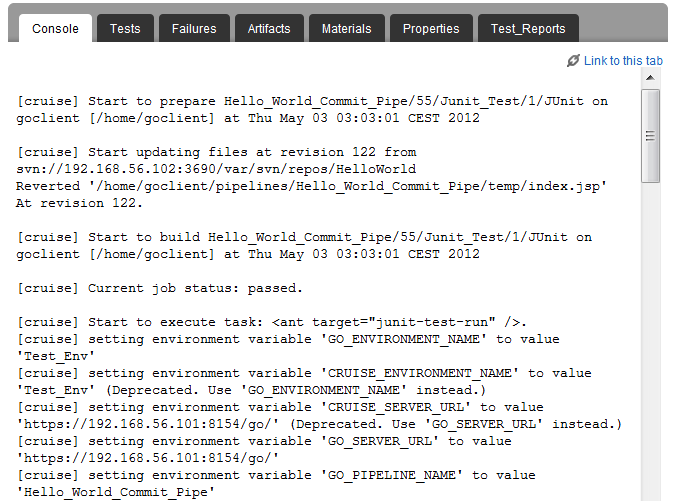
\includegraphics[scale=0.5]{Grafiken/go_005_Job_Console_cut.PNG}}\hfill
\fbox{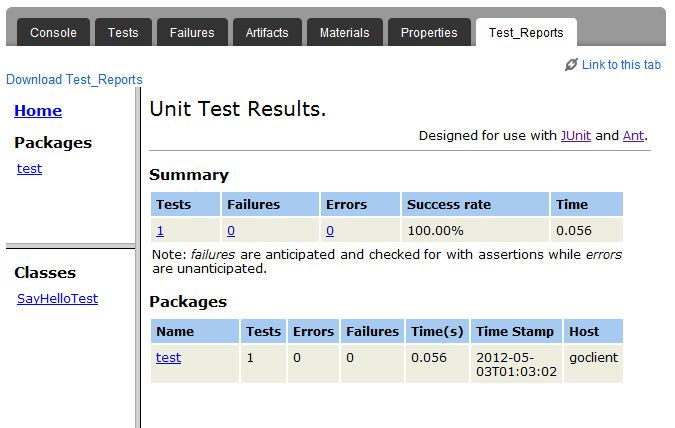
\includegraphics[scale=0.5]{Grafiken/go_008_Job_JUnit-Test_cut.PNG}}
\caption[Log-Datei und JUnit Test-Report in \go]{Darstellung der Konsolenausgabe und des JUnit Test-Reports.}\label{pic:go_test_report}
\end{figure}

%\begin{wrapfigure}{r}{0.33\textwidth}
%\centering
%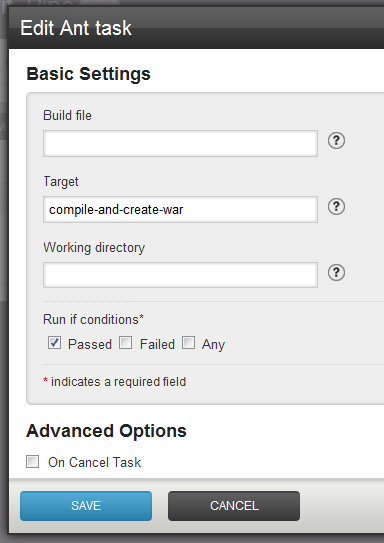
\includegraphics[scale=0.6]{Grafiken/go_ant_task.PNG}
%\caption{Ant-Task}\label{fig:go_ant}
%\end{wrapfigure}

%In Abbildung~\ref{fig:go_ant} wird die Konfiguration des Ant-Tasks gezeigt.

F�r die Test-Pipeline ist der erste Task der \comstage\ das Kompilieren und Packen der Binaries in Form eines War-Files. Hierf�r wird der Ant-Taks genutzt. Dieser erwartet die \texttt{build.xml} und das Ant-Target, welches die Ant-Kommandos enth�lt. Das Target \texttt{compile-and-create-war} muss mit dem in der \texttt{build.xml} �bereinstimmen, wie nachfolgendes Listing zeigt.
\lstset{language=ant}
\vspace{\baselineskip}
\begin{lstlisting}[caption={Ant-Target}]
<target name="compile-and-create-war">
   <.... />
</target>
\end{lstlisting}
\vspace{\baselineskip}
Die in diesem Task auszuf�hrenden Aufgaben wie kompilieren, testen, packen werden von Ant �bernommen. Auf diese Weise k�nnen in \go\ alle Aufgaben f�r die \comstage\ umgesetzt werden. Neben Ant werden auch NAnt und Rake unterst�tzt. M�ssen andere Tools genutzt werden, \zb\ weil ein Projekt auf Maven setzt, ist dies �ber ein \emph{Custom-Command} m�glich.  �ber \emph{Custom-Command} k�nnen beliebige Kommandos auf der Systemkonsole ausgef�hrt werden und so Systemprogramme, Shell-Skripte oder andere Systeme angesprochen werden, die f�r die \dpipe\ Aufgaben �bernehmen.

F�r Anwendungen, die auf das Build-Tool Ant setzen, ergeben sich eine ganze Reihe von M�glichkeiten, Tests und Analysen auf der Quellcode-Basis durchf�hren zu lassen. So kann \zb\ ein Sonar-Server �ber ein Ant-Plugin eingebunden werden, um die statische Code-Analyse zu erm�glichen und Parameter wie Testabdeckung und Code-Style analysieren zu lassen. Die Testabdeckung l�sst sich bei Sonar �ber den Anteil durch Testf�lle abgedeckter Codezeilen als auch �ber die den Anteil der im Test durchlaufenen Kontrollflusspfade berechnen.\footnote{Vgl. \cite{sonar_testcoverage}}

Aus den durchgef�hrten Tests lassen sich so Quality-Gates definieren, welche �ber die Qualit�t der Anwendung wachen. Dies spielt eine Rolle bei der Entscheidung, ob der neue Stand der Quellcode-Basis die notwendigen Qualit�tskriterien erf�llt, um in die nachfolgende Stage oder in die Produktivumgebung weitergereicht werden zu k�nnen. Ein Beispiel f�r ein Quality-Gate ist die Definition eines Merkmals wie die Testabdeckung. Hier k�nnte dann, je nach Definition, ein Wert von mindestens $70~\%$ bestimmt werden, der erreicht werden muss, bevor die Pipeline von der \comstage\ in die \acstage\ �bergehen kann. Dieses Kriterium kann aber nur eines von weiteren sein, um den Weiterfluss innerhalb der \dpipe\ zu steuern.

Die \acstage\ wurde im Testprojekt einfach gehalten. Sie diente vornehmlich der Erprobung der Testversion und wurde aus diesem Grunde nicht weiter vertieft. Umgesetzt wurden im JWebUnit ein einfacher Test, der die Anforderung an die Hello-World-Anwendung pr�ft und testet, ob die Nachricht \mycite{Continuous Delivery Test Web Project} beim Aufrufen der Seite erscheint. JWebUnit ist ein auf Java basierendes Test-Framework f�r Web-Anwendungen von SourceForge. JWebUnit vereint dabei die Frameworks HtmlUnit und Selenium durch eine einheitliche Schnittstelle, ben�tigt aber JUnit zur Ausf�hrung.\footnote{Vgl. \cite{SourceForge}} F�r den Aufbau der \dpipe\ besitzt dieser Test aber eine hinreichende Gr��e, um die Funktionsweise der Pipeline zu testen.

Nachfolgendes Listing zeigt diesen Test:
\lstset{language=java}
\vspace{\baselineskip}
\begin{lstlisting}[caption={Smoke-Test mit JWebUnit}]
\begin{lstlisting}
public class IndexPageTest {
  @Before
    public void prepare() {
      setBaseUrl("http://192.168.56.102:8080/HelloWorld");
    }
  @Test
  public void openIndexPage() {
    beginAt("index.jsp");
    assertTitleEquals("Continuous Delivery Test Web Project");
    assertElementPresent("sayHelloTitel");
  }
}
\end{lstlisting}
\vspace{\baselineskip}
Die Ausf�hrung wird als Ant-Task in die \dpipe\ von \go\ eingebaut. Auf Ebene von \go\ muss hier lediglich das Ant-Target \texttt{jwebunit-test-run} angegeben werden. Um JWebUnit nutzen zu k�nnen, m�ssen Jar-Dateien von JWebUnit auf dem ausf�hrenden Agent-System verf�gbar sein und der Pfad zum Classpath, \zb\ per \texttt{build.xml}, hinzugef�gt werden.

\lstset{language=ant}
\vspace{\baselineskip}
\begin{lstlisting}[caption={Einbinden von JWebUnit in Ant}]
...
<property name="jwebunit-home" value="/opt/JWebUnit" />
...
<target name="jwebunit-test-run">
  <javac srcdir="JWebUnit" destdir="JWebUnit">
    <classpath>
      <path refid="junit-jar" /><path refid="jwebunit-classpath" />
    </classpath>
  </javac>
  <mkdir dir="jwebunitTestReports" />
  <junit haltonfailure="true" includeantruntime="true" 
      printsummary="true" showoutput="true">
    <classpath>
      <pathelement location="JWebUnit"/>
      <path refid="junit-jar" />
      <path refid="jwebunit-classpath" />
    </classpath>
    <formatter type="xml" />
    <batchtest fork="yes" todir="jwebunitTestReports">
      <fileset dir="JWebUnit"><include name="**/*Test*.class" />
    </batchtest>
  </junit>
  <junitreport todir="jwebunitTestReports">
    <fileset dir="jwebunitTestReports" includes="TEST*.xml" />
     <report todir="jwebunitTestReports" />
   </junitreport>
</target>
\end{lstlisting}
\vspace{\baselineskip}

Nach der Kompilierung der Tests wird ein Verzeichnis angelegt, in welches JUnit die generierten Testberichte im XML-Format ablegen kann. Nach dem Durchlauf der Tests werden diese dann von \lstinline$<junitreport>$ in formatierte HTML-Dateien umgewandelt. Abbildung~\ref{pic:go_add_junit_reports} zeigt, wie Berichte im HTML-Format in die Oberfl�che eingebunden werden k�nnen. Berichte sind dabei Artefakte der \dpipe , die beim Durchlauf dieser entstehen. Artefakte verbleiben, sofern nicht anders spezifiziert, im Arbeitsverzeichnis des Agents und werden bei der n�chsten Aktivierung des Agents gel�scht. Um Artefakte f�r die weitere Verwendung innerhalb der Pipeline verwenden zu k�nnen, m�ssen diese auf den \go -Server �bertragen werden. Dies kann �ber die Konfiguration von \emph{Artifacts} erreicht werden. In der Abbildung werden die Testberichte von JMeter als Test-Artefakte auf den Server �bertragen. �ber die Konfiguration eines \emph{Custom Tab} kann dann eine beliebige HTML-Seite mit den Testergebnissen eingebunden werden. Das Entwicklerteam hat so einen schnellen Zugriff auf die Testauswertung.

Da jeder so eingef�gte Bericht an die Instanz der Pipeline gebunden ist, k�nnen auch alle Berichte der vorhergehenden Durchl�ufe aufgerufen werden. Auf diese Weise werden Regressionen an der Quellcode-Basis festgestellt. Verschlechtern sich die Ergebnisse wie die Anzahl von Fehlschl�gen, die Gr��e der Testabdeckung oder die Durchlaufzeit, kann dies �ber die Historie n�her inspiziert werden und eine bestimmte �nderung an der Code-Basis als Ursache identifiziert werden. \go\ bietet hier eine kontinuierliche Qualit�tssicherung, wie sie von \ci\ vorgeschlagen wird.



Ein effektiver Ansatz, Akzeptanztests in die \dpipe\ einzubauen, ist das \emph{B}ehavior \emph{D}riven \emph{D}evelopment (BDD). Bei BDD werden vor Beginn der Entwicklungsarbeit, Akzeptanzkriterien aus verbaler Sprache in mehreren Iterationen, in ausf�hrbarere Testf�lle umgeformt.\footnote{Vgl. \cite{North}} Der Vorteil, Akzeptanzkriterien zu Beginn der Entwicklung einer Anwendung als automatisiert durchf�hrbare Tests zu definieren, kommt bei \cd\ sehr gut zum Tragen. Die so entwickelten Akzeptanztests k�nnen verwendet werden, um innerhalb der \dpipe\ entscheiden zu k�nnen, ob alle f�r ein Release notwendigen Akzeptanzkriterien erf�llt werden. Da die \dpipe\ bei jeder �nderung der Quellcode-Basis aktiviert wird, werden auch alle definierten und als Test implementierten Akzeptanzkriterien gepr�ft. 

\begin{figure}
 \subfigure[Log-Datei]
  {\fbox{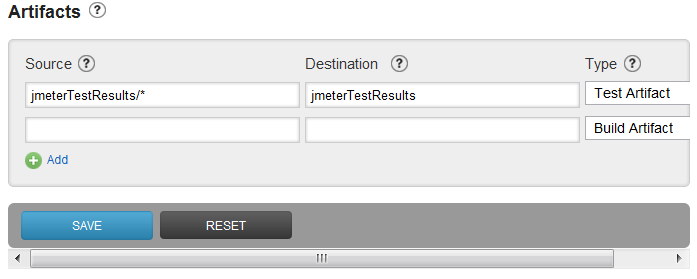
\includegraphics[scale=0.5]{Grafiken/go_008_Pipeline_Edit_Stage_Job_Artifacts_cut.PNG}}}
  \hfill
  \subfigure[JUnit Testbericht]
  {\fbox{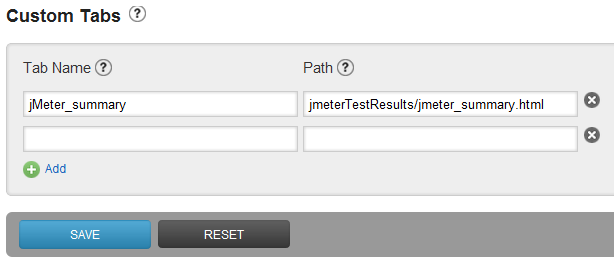
\includegraphics[scale=0.5]{Grafiken/go_009_Pipeline_Edit_Stage_Job_CustomTabs_cut.PNG}}}
  \caption[Testberichte in \go\ einbinden]{JUnit-Testberichte in die OBerfl�che von \go\ einbinden.}\label{pic:go_add_junit_reports}
\end{figure}

In \go\ lassen sich Akzeptanztests sehr gut in Form der \acstage\ einbauen. Die Entscheidung, ob in die Produktionsumgebung bzw. in die 
\uastage\ geliefert wird, muss in \go\ durch ein Skript realisiert werden. Dieses muss die vorliegenden Test-Berichte analysieren und aggregieren k�nnen. Dieser Vorgang sollte einen Qualit�tsindex erzeugen k�nnen, der der Pipeline einen Messwert f�r die Entscheidungsfindung liefert. Weniger Komplex kann dies auch als manueller Vorgang gestaltet werden. Nach dem Durchlauf der Akzeptanztests wird dem Entwicklungsteam eine Nachricht �ber den Abschluss der Stage zugesandt. Ein Teammitglied pr�ft dann die Testberichte und entscheidet, ob diese Version reif f�r die Produktion ist.

\paragraph{Deployment}

Wie das Ausrollen einer Anwendung in eine bestimmte Umgebung organisiert werden kann, gibt \go\ nicht vor. Zur Unterst�tzung wird aber folgendes geboten:

\begin{itemize}
\item \emph{Custom-Command} durch die freie Verwendung der Systemkonsole \zb\ in Verbindung mit Shell-Skripten.
\item \emph{Ant Taks}, bzw. auch die unterst�tzten Tools NAnt und Rake, in Verbindung mit Plug-Ins f�r diese Build-Tools, die das Deployment in bestimmte Server-Umgebungen erm�glichen.
\item \go -Agent selbst als Ausf�hrungsumgebung der Software.
\end{itemize}

In Verbindung mit \emph{Custom-Command} k�nnen Werkzeuge wie Chef angesprochen werden, um ein Deployement zu organisieren. So bietet das Plugin \emph{knife-ec2}\footnote{Mehr Informationen zu knife-ec2 unter: \url{https://github.com/opscode/knife-ec2}} f�r Chef die M�glichkeit, Instanzen von Amazons EC2 direkt provisionieren zu k�nnen\footnote{Vgl. \cite{Stoyanov2012}, interne Quelle und \cite{Timberman2012}}, wie folgendes Kommando zeigt:

\lstset{language=bash}
\vspace{\baselineskip}
\begin{lstlisting}[caption={Knife-Anweisung f�r EC2 Instanz}]
knife ec2 server create -I ami-3323f25a -S homeKey.pem 
   -f t1.micro -i ./.chef/homeKey.pem -x ubuntu -r role[programXYZ]
\end{lstlisting}
\vspace{\baselineskip}
Dabei enth�lt \lstinline$role[programmXYZ]$ Anweisungen, die Teile eines Kochbuchs von Chef sind. Innerhalb einer Rolle werden dann alle Anweisungen zusammengefasst, um ein System zu konfigurieren. Auf diese Weise k�nnen \zb\ ben�tigte Server und Infrastruktur erstellt werden, um die Anwendung zu testen oder in Produktion zu bringen.\footnote{Vgl. \cite{Gheorghiu2010}}

Eine weitere M�glichkeit, die \go\ bietet, aber nicht die Flexibilit�t von Chef mitbringt, ist die Verwendung eine Plugins f�r Ant, um eine Web-Anwendung zu deployen. In der Test-Pipeline wird ein Plugin f�r Tomcat verwendet, um mit dem Tomcat-Manager zu kommunizieren. Nachfolgendes Listing zeigt die Deyploy-Anweisung f�r Ant, um das War-File der Hello-World-Anwendung in eine Tomcat-Instanz zu deployen: 

\lstset{language=ant}
\vspace{\baselineskip}
\begin{lstlisting}[caption={Tomcat-Deployment mit Ant}]
<property name="tomcat-manager-url" 
  value="http://~\$~{tomcat-server-ip}:8080/manager" />
...
<path id="catalina-ant-classpath">
  <pathelement location="~\$~{ant-lib-dir}/catalina-ant.jar"/>
</path>
...
<taskdef name="deploy" 
   classpathref="catalina-ant-classpath"
   classname="org.apache.catalina.ant.DeployTask" />
...
<target name="deploy-tomcat-from-compile-pipe" depends="get-war-file">
  <deploy url="~\$~{tomcat-manager-url}" username="~\$~{tomcat-username}"
    password="~\$~{tomcat-password}" path="/HelloWorld"
    war="file:/home/goclient/pipelines/"
      "~\$~{go.GO_PIPELINE_NAME}/~\$~{deploy-war-folder}"  
    update="true">
  </deploy>
</target>
\end{lstlisting}
\vspace{\baselineskip}

Zumindest f�r eine Testumgebung und f�r kleinere Anwendungen mit fixer Infrastruktur ist dies eine einfache M�glichkeit, eine Web-Anwendung zu deployen. Die dritte M�glichkeit bedingt die Nutzung des \go -Agents als Ausf�hrungsumgebung. 

\begin{wrapfigure}{r}{0.33\textwidth}
\centering
\fbox{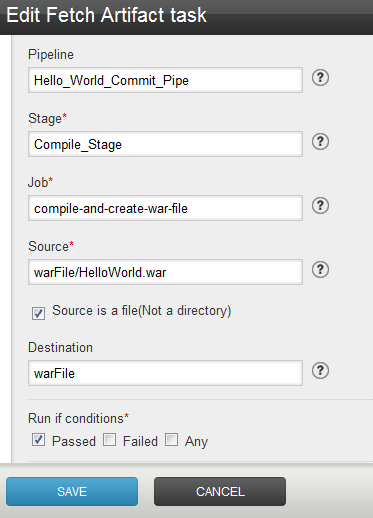
\includegraphics[scale=0.6]{Grafiken/go_010_Pipeline_Edit_Stage_Job_FetchTask_cut.PNG}}
\caption[Artefakte in \go\ wiederverwenden.]{Artefakt einer anderen Stage wiederverwenden.}\label{fig:go_fetch}
\end{wrapfigure}

Alle Anweisungen zur Anpassung der Infrastruktur, an die die Ausf�hrung der Anwendung gekn�pft ist, k�nnen dann �ber \emph{Custom-Command} oder Shell-Scripte ausgef�hrt werden. Ein Shell-Skript sollte dann Teil der Versionskontrolle sein. �nderungen k�nnen so auch extern, \zb\ in der Entwicklungsumgebung vorgenommen werden. Die aktuelle Version des Shell-Skripts wird durch das Agent-System als Teil des auszuf�hrenden Jobs in das Arbeitsverzeichnis geladen und kann dann von dort aufgerufen werden. Sind alle Anpassungen vorgenommen, k�nnen die Binaries ausgef�hrt oder wie Beispielprojekt in das Arbeitsverzeichnis des Tomcat-Servers kopiert werden. Der Tomcat stoppt die aktuell ausgef�hrte Version der der Anwendung, entpackt das neue Archiv und startet die Anwendung neu. Um diesen Schritt vollziehen zu k�nnen, m�ssen Binaries, die in einer anderen Stage kompiliert wurden, in das aktuelle Arbeitsverzeichnis kopiert werden. Dieses Szenario ist allerdings nur auf kleinere Projekte mit kleinerer Testinfrastruktur bzw. auf ein paar wenige Projekte begrenzt, da, je nach Lizenz, nur 10 bzw. 25 Agents verwendet werden k�nnen. Bei der kostenfreien Communit-Version sind es lediglich drei Agents. 

\subsubsection{Beurteilung}

\paragraph{Funktionalit�ten}

\go\ kann auf den Betriebssystemen Microsoft Windows, Mac~OS~X, Linux und Solaris ausgef�hrt werden. M�glich wird dies durch die Plattformunabh�ngigkeit der Java-Runtime, auf welcher \go\ l�uft. \go\ bietet eine umfassende Abbildung einer \dpipe\ mit der Modellierung der \comstage , \acstage , \uastage , \capstage\ und \prodenv . Jobs k�nnen parallel ausgef�hrt werden, wodurch das Konzept von Fail-Fast m�glich wird. Um die Aufgaben \emph{compile}, \emph{test} und \emph{deploy} verwirklichen zu k�nnen, wird Ant, NAnt und Rake unterst�tzt. Andere Tools oder Shell-Skripte k�nnen als Kommando f�r die Systemkonsole mittels \emph{Custom-Command} angesto�en werden.

Die Stages werden der Reihe nach ausgef�hrt. Eine Pipeline wird durch die Ereignisse Material oder Pipeline angesto�en. Letzteres erm�glicht den Aufbau von Baumstrukturen f�r Pipelines und die Abbildung komplexerer Lieferprozesse.

Um komplexe Deployment-Szenarien f�r Test- oder Produktivumgebungen l�sen zu k�nnen, bietet \go\ mit dem Ant-Taks sowie dem \emph{Custom-Command} verschiedene M�glichkeiten, dieses durchf�hren zu k�nnen. Dabei k�nnen Tools wie Chef in Verbindung mit der EC2 von Amazon genutzt werden, um sich auf einfache Weise mit ben�tigten Infrastrukturen f�r Test- oder Produktivumgebung versorgen und konfigurieren zu k�nnen. Auch �ber Ant ist das Deployment, \zb\ �ber den Catalina-Ant-Task, realisierbar. Eine letzte M�glichkeit ist die Verbindung von Ausf�hrungsumgebung und \go -Agent auf einem System. Dabei k�nnen die notwendigen Anpassungen als \emph{Custom-Command} in der Pipeline-Konfiguration oder als Shell-Skript in das \verskont\ abgelegt werden. Der Agent hat dann direkte Kontrolle auf das System und kann Anwendungen installieren, starten oder stoppen.

\go\ bietet damit ein vollst�ndiges \cd -System an, welches \ci\ integriert und das Konzept so erweitert, dass entweder externe Deployment-L�sungen angesprochen werden k�nnen oder aber der \go -Agent selbst zu Ausf�hrungsumgebung wird.

\paragraph{Zuverl�ssigkeit}

\go\ wird seit Ende September in der Version $12.3$ angeboten. F�r die Erprobung im Juni und Juli 2012 kam dementsprechend Version $12.2$ zum Einsatz. \go\ befindet sich als propriet�r vertriebenes Produkt in der st�ndigen Weiterentwicklung. Es kann davon ausgegangen werden, dass dieses Produkt auch in den n�chsten Jahren weiterentwickelt, gewartet und verbessert wird. Treten im Programmablauf Fehler auf, werden diese geloggt. Das Problem mit der Testversion ist vornehmlich durch die geringe Ausstattung des Testsystems mit 1280~MB~RAM aufgetreten.

Die Konfigurationseinstellung von \go\ kann durch ein Back-up im Administrationsbereich der Oberfl�che gesichert werden. Hierzu geh�ren dann alle Einstellungen wie Pipelines, Nutzer, Rollen, Umgebungen, registrierte Agent-Systeme und weitere Informationen. Eine Sicherung von Artefakten erfolgt nicht, was auch nicht notwendig erscheint. Alle Artefakte lassen sich durch Aktivierung einer Instanz der Pipeline mit der gesuchten Revisionsnummer des \verskont\ wiederherstellen.

\paragraph{Benutzbarkeit}

\go\ orientiert sich eng am Konzept von \cd . Pipelines und Stages werden auch in \go\ an das Konzept angelehnt bezeichnet, was den Einstieg in die Konfiguration erleichtert. Die gesamte Anwendung kann �ber die Oberfl�che bedient und konfiguriert werden. Es ist aber auch m�glich, die Systemkonfiguration in Form einer XML-Datei in die Anwendung zu laden. Das erm�glicht die Konfigurationen f�r \go\ selbst unter die Versionskontrolle zu stellen. Diese M�glichkeit l�sst die \dpipe\ noch stabiler werden. Schl�gt der Lieferprozess nach einer �nderung der Konfiguration fehl, kann die alte Konfiguration sehr schnell wiederhergestellt werden.

Die Oberfl�che selbst zeigt den aktuellen Zustand der Pipeline sowie die Ergebnisse der letzten Durchl�ufe an. Der Nutzer erh�lt ein sehr schnelles Feedback �ber die derzeit vom System ausgef�hrten Aufgaben. Symbole wie \emph{Play} und \emph{Pause}, mit denen ein Prozess manuell angesto�en bzw. pausiert werden kann, erleichtern die Bedienung der Pipelines. Statusinformationen werden �ber die farbigen Elemente mit den Farben gr�n, rot und gelb. Wird eine Pipeline bzw. ein Job einer Pipeline ausgef�hrt, wird dies als gelb-animierter Balken in der Oberfl�che gezeigt.

Die Oberfl�che ist durch das Layout und die Farbgestaltung klar strukturiert. Der Nutzer kann sich jederzeit orientieren und eine intuitive Bedienung ist m�glich. So sind Verbindungen zwischen �bersichten und Detailansichten klar und einheitlich durch Anklicken des Titels geregelt.

Die Dokumentation von \go\ ist nach Rollen gegliedert und erleichtert so den Einstieg in die Anwendung. Mit der Formulierung \mycite{As a developer, i want to ...} werden die typischen Aufgaben eingeleitet, die \zb\ ein Entwickler mit \go\ gerne erledigen m�chte, wie \mycite{... watch what's currently building}.\footnote{Vgl. \cite{ThoughtWorksInc.}}

\paragraph{Effizienz}

Die empfohlene Systemkonfiguration f�r \go\ ist ein 2~GHz Prozessor.  F�r den Server werden mindestens 1 bis 2~GB RAM und f�r das Agent-System 128 bis 256~MB vorausgesetzt.  Der Probebetrieb erfolgte in einer virtuellen Umgebung. Das Host-System war ein mit 4~GB Arbeitsspeicher ausgestatteter Laptop mit Windows~7. Um das Host-System nicht zu �berbeanspruchen, konnten die virtuellen Systeme nicht mit der empfohlenen, sondern nur mit der minimal geforderten Speichergr��e versehen werden. Zu Beginn ist der Server mit 1024~MB und der Agent mit 256~MB ausgestattet worden. Da der Server am Anfang der Erprobung instabil lief und bei der Ausf�hrung einer Stage Speicherprobleme auf der Konsole ausgab, wurde der Speicher auf 1280~MB angehoben, was die Probleme beseitigte. Der \go -Agent wurde gleich mit der empfohlenen Gr��e versehen, sodass hier im gesamten Verlauf keine Probleme auftraten.

Ein weiteres Merkmal, welches bei der Planung Ber�cksichtigung finden sollte, ist der notwendige Plattenplatz, um Artefakte ablegen zu k�nnen. Jede Aktivierung der Pipeline produzierte Testberichte, Log-Dateien und Binaries. Je h�ufiger die Pipeline aktiviert wird, desto mehr Plattenplatz muss zur Verf�gung stehen, um die anfallenden Artefakte speichern zu k�nnen. Eine Webanwendung, die in ihrer kompilierten Form \zb\ 30 bis 40~MB Platz beansprucht, w�rde bei gesch�tzten 100 �nderungen der Quellcodebasis 3 bis 4~GB Speicherplatz ben�tigen. Ein Team, welches aus 5 Entwicklern besteht und t�glich einmal die �nderungen commited, erreicht dieses Volumen in 4 Wochen. Laufen 10 oder 20 Projekte parallel, kommen so in nur 4 Wochen 30 bis 80~GB zusammen.

Da die \dpipe\ in \go\ mit einer beliebigen Version der Quellcode-Basis jederzeit auch die gleichen Ergebnisse produziert, sind nur die zuletzt erzeugten Artefakte von einem besonderen Interesse. �lter Artefakte k�nnen gel�scht werden. \go\ bietet die M�glichkeit, den Speicherplatz f�r Artefakte zu limitieren. Dabei wird regelm��ig gepr�ft, wie viel Restspeicher auf dem System noch vorhanden ist. Eine entsprechende Konfiguration k�nnte so beim Erreichen einer Untergrenze von 10~GB Restspeicher alle Artefakte so lange l�schen, bis der freie Plattenspeicher wieder mindestens 25~GB betr�gt.

\paragraph{Portabilit�t}

Eine Erweiterung von \go , \zb\ durch Plug-ins, ist nicht m�glich. Eine �nderung der Anwendung ist nicht m�glich. Im Probelauf wurde aber keine Funktionalit�t vermisst, welche eine �nderbarkeit der Anwendung erw�nscht h�tte.

Die Installation von \go\ war einfach und unkompliziert. Sofern die notwendige Infrastruktur in Form der Java-Runtime von Oracle und Subversion installiert ist, kann der \go -Server starten. Je nach Tasks, die in der \dpipe\ ausgef�hrter werden sollen, m�ssen zus�tzliche Werkzeuge auf dem Agent-System installiert werden. Im Testprojekt waren diese, zus�tzlich zu den schon genanten, JUnit Ant-Plugin, JWebUnit Ant-Plugin, Catalina Ant-Plugin und das JMeter Ant-Plugin.

\go\ kann als JAR-File direkt von der Konsole mit \lstinline$java -jar go.jar$ gestartet werden. Der \go -Agent muss zus�tzlich noch die Adresse des \go -Servers als Parameter �bergeben bekommen: \lstinline$java -jar agent-bootstrapper.jar <go-server-host>:<port>$

Die Dokumentation gibt alle notwendigen Vorgaben zum Systembetrieb, sodass die Installation und die Konfiguration problemlos verlaufen sind. Der \go -Server, im Gegensatz zum \go -Agent, ben�tigt reichlich Speicherplatz. Bei entsprechender Hardware-Konfiguration k�nnen aber mehrerer Agents auf dem selben System parallel gestartet und am Server angemeldet werden.

\subsection{\dpl\ von Etsy}\label{chap_dpl}

\dpl\ wurde von Etsy entwickelt, um �nderungen der eigenen Anwendung, den  Etsy Web-Shop\footnote{Mehr Information zu Etsy unter: \url{http://www.etsy.com/}}, schnellstm�glich in die Produktivumgebung zu bringen. Einen ma�geblichen Anteil an der Entwicklung von \dpl\ hatte Erik Kastner, der \dpl\ �ber einen Eintrag vom 29.07.2011 auf dem Entwickler-Blog\footnote{Entwickler-Blog von Etsy unter: \url{http://codeascraft.etsy.com/}} von Etsy frei zug�nglich\footnote{\dpl\ auf GitHub unter: \url{https://github.com/etsy/deployinator}} machte und unter die MIT-Lizenz\footnote{Mehr Informationen zur MIT-Lizenz unter: \url{http://opensource.org/licenses/mit-license.php}} stellte.\footnote{Vgl. \cite{codeascraft}} Durch diesen Lizenztyp ist es m�glich, \dpl\ \zb\ frei zu verwenden, zu kopieren oder zu �ndern.\footnote{Vgl. \cite{mit_license}}

Kastner fasst \dpl\ in einem Satz wie folgt zusammen: \mycite{one button web-based deployment app}. Vor \dpl\ ben�tigte Etsy f�r ein Deployment ihrer Web-Anwendung in die Produktivumgebung drei Entwickler und einen Verantwortlichen aus dem IT-Betrieb. Mit \dpl , so Kastner, war es Etsy m�glich geworden, das Deployment auf unter zwei Minuten zu reduzieren, das nun praktisch von jedem Teammitglied durchgef�hrt werden kann. Etsy deployt die Anwendung seit dem mehrmals am Tag.\footnote{Vgl. \cite{codeascraft}}

Die Entwicklungsziele von \dpl\ fasst Kastner so zusammen:

\begin{itemize}
\item Die Anwendung ist Web-basierend,
\item loggt Ereignisse,
\item l�sst sich in die Infrastruktur von Etsy integrieren,
\item nutzt IRC und E-Mail, um das Team zu informieren,
\item ist transparent im Hinblick auf die ausgef�hrten Aktionen und
\item die Integration in das Monitoring-System von Etsy ist m�glich.
\end{itemize}

\subsubsection{Konzept von \dpl}

Als Web-Anwendung l�uft \dpl\ als Ruby-Anwendung, welche auf das Sinatra-Framework\footnote{Weiter Informationen zum Sinatra-Framework unter: \url{http://www.sinatrarb.com/}} aufbaut. Deployinator erm�glicht die Ausf�hrung von Shell-Skripten und Kommandos auf der Systemkonsole. Um verschiedene Projekte bzw. Anwendungskomponenten wie Web oder Datenbank parallel verwalten zu k�nnen, lassen sich Stacks mit eigenen Konfigurationen definieren. Jeder Stack kann wiederum f�r verschiedene Umgebungen konfiguriert werden. So ist \zb\ die Definition von \emph{Test} und \emph{Produktion} m�glich. Technisch ist ein Stack ein Ruby-Modul, f�r das bestimmte Methoden zu implementieren sind. Durch dieses Modul wird der Stack konfiguriert.

Das Konzept von \dpl\ unterscheidet sich wesentlich von \go . \dpl\ erg�nzt ein bestehendes System f�r \ci . Das Kompilieren und Durchf�hren automatisierter Tests steht hier nicht im Fokus. Vielmehr soll \dpl\ das Ausrollen einer Anwendung in Produktivumgebung dahin gehend unterst�tzen, dass es dem Entwicklungsteam eine Oberfl�che bereitstellt, Deployment-Skripte ansto�en zu k�nnen.

\subsubsection{Funktionen von \dpl}

\paragraph{Management der \dpipe}

\begin{figure}
\fbox{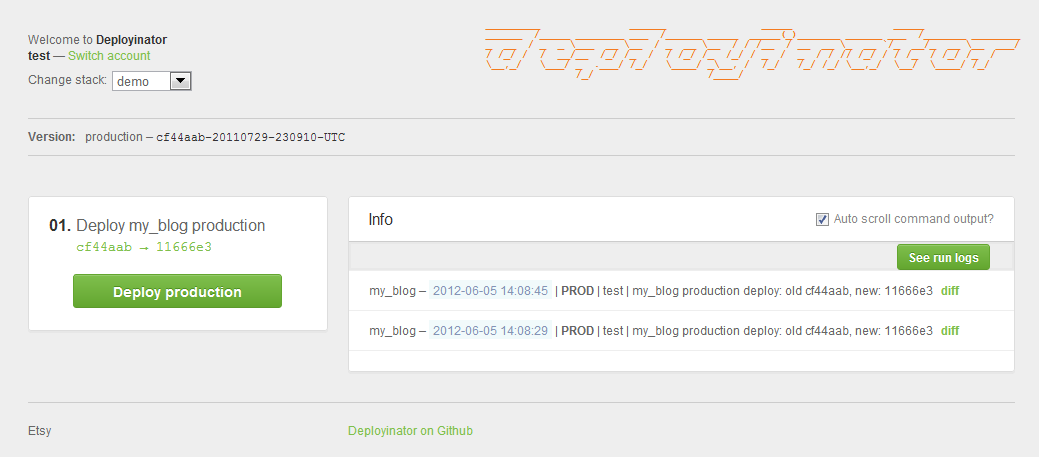
\includegraphics[width=\linewidth]{Grafiken/dpl_front_page.png}}
\caption[Oberfl�che \dpl]{Oberfl�che von \dpl .}\label{dpl_frontpage}
\end{figure}

Die Modellierung von Pipelines, wie es in \go\ m�glich ist, kann derart mit \dpl\ nicht umgesetzt werden. Das bedeutet nicht, dass keine \dpipe\ mit \dpl\ m�glich ist. Ferner ist \dpl\ die geeignete Erweiterung eines CI-Systems. Die Hauptseite von \dpl\ ist in Abbildung~\ref{dpl_frontpage} dargestellt. \dpl\ erzeugt je Umgebung eines Stacks einen Button auf der Web-Oberfl�che. Bei Bet�tigung des Buttons werden die im Modul definierten Aktionen, wie der Aufruf von Kommandos auf der Systemkonsole, durchgef�hrt. Demnach werden alle Prozesse manuell angesto�en. Hat das CI-System alle Testkriterien in Form der Komponenten- und Akzeptanz-Tests sowie der statischen Code-Analyse durchgef�hrt, kann dies durchaus gew�nscht sein. Im Fall der \uastage\ kann sich dann das Testteam die aktuelle Version der Anwendung zum Testen in die Testumgebung deployen. Diese entspricht einem \ssp .

Relevante Ausgaben bei der Durchf�hrung einzelner Aktionen k�nnen in ein Log-File geschrieben werden. Es h�ngt aber von der jeweiligen Konfiguration ab, ob Informationen in das Log-File geschrieben werden. \dpl\ stellt hierf�r lediglich Methoden bereit, die dies erm�glichen. Das Log-File selbst wird auf der Weboberfl�che eingeblendet. Dabei aktualisiert es sich selbst in kurzen Abst�nden, wodurch der Eindruck einer aktiven Systemkonsole entsteht.

Obwohl \dpl\ konzeptionell ein CI-System erweitert, ist es m�glich, Build und Test-Prozesse auch mit \dpl\ umzusetzen. Allerdings ist dabei kein automatisches triggern durch �nderungen an der Code-Basis m�glich. Alle definierten Prozesse m�ssen �ber die Oberfl�che manuell angesto�en werden.

\paragraph{Stages}

\dpl\ integriert Git f�r Aufgaben der Versionsverwaltung. Dabei ist es aber auch ohne Probleme m�glich, auch andere Systeme wie Subversion zu verwenden und diese �ber die Systemkonsole von \dpl\ ansprechen zu lassen. Im Testprojekt wird die Code-Basis aus Subversion geladen. Nachfolgendes Listing zeigt die Einbindung von Shell-Skripten in das Stack-Modul:

\lstset{language=ruby}
\vspace{\baselineskip}
\begin{lstlisting}[caption={Stack-Modul von Deployinator}]
def my_test_build_and_deploy(options={})
  # last deployed version  
  old_build = %x{cat ~\$~userHome/current_deployed_version}
  # current version on 
  cur_build = %x{svn info 
    svn://192.168.56.102:3690/var/svn/repos/HelloWorld 
    | grep '^Revision:' | awk '{print ~\$~2}'}
  # run build-script
  run_cmd %Q{~\$~userHome/build_war.sh}
  # log the deploy
  log_and_shout :old_build => old_build, :build => cur_build
end
\end{lstlisting}
\vspace{\baselineskip}
Das Build-Skript, welches hier angesto�en wird, l�dt zu erst die aktuelle Quellcode-Basis aus dem Versionsverwaltungssystem. Die derzeit ausgef�hrte Version wird in einer lokalen Verzeichnisstruktur gesichert. Abildung~\ref{fig:dpl_stacks} zeigt zwei implementierte Stacks. Jeder dieser Push-Buttons aktiviert eine eigene Methode im Stack-Modul.

\begin{wrapfigure}{r}{0.33\textwidth}
\centering
\fbox{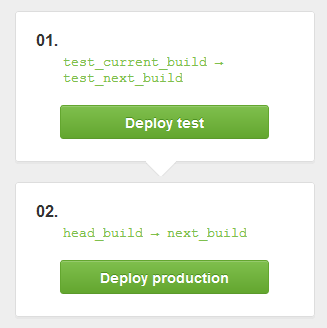
\includegraphics[width.3\linewidth]{Grafiken/dpl_stack.png}}
\caption[Stacks mit Push-Button in \dpl ]{Stacks mit Push-Button in \dpl .}\label{fig:dpl_stacks}
\end{wrapfigure}

\paragraph{Deployment}

\dpl\ wurde besonders auf die schnelle Aktivierung von Deployment-Skripten bzw. zur Aktivierung von Werkzeugen, die das Deployment �bernehmen, konzipiert. Im Fokus steht hier also viel mehr deren Ansto�, als eine Unterst�tzung des Deployments selbst. \dpl\ kann aber deshalb als leichtes Self-Service-Portal angesehen werden.

Perspektivisch betrachtet l�sst sich \dpl\ auch in einer Situation nutzen, in der ein direktes Deployment in die Ausf�hrungsumgebung des Kunden nicht m�glich ist. Dabei kann auf Kundenseite ein vorkonfigurierter \dpl\ installiert werden. Einem Testteam des Kunden kann mit \dpl\ die M�glichkeit in gegeben werden, sich f�r Testzwecke selbst mit der aktuellen Version zu versorgen. Die aktuelle Version k�nnte dann durch \dpl\ in die Testumgebung zu deployt und ausgef�hrt werden. Die Anwendung kann dann durch den Kunden explorativ untersucht und abgenommen werden.

Dieses Szenario ist auch f�r die Produktivumgebung denkbar. So fern ein neues Feature durch den CI-Prozess gegangen ist und alle vereinbarten Akzeptanzkriterien erf�llt sind, wird die neue Version in ein f�r den Kunden erreichbares Repository ausgeliefert. Der Kunde kann hier�ber durch das CI-System informiert werden. Die Testabteilung des Kunden ruft dann die Oberfl�che von \dpl\ auf und kann das Deployment aktivieren und die neue Version testen. Wird die neue Version akzeptiert, kann der Programm-Manager des Kunden bzw. der IT-Betrieb das Deployment in die Produktivumgebung ansto�en. Deployinator kann dann so konfiguriert werden, dass adesso als Lieferant in diesem Szenario �ber das Ausliefern in die Produktivumgebung durch das System informiert wird. Dies kann \zb\ aus vertragsrechtlichen oder abrechnungstechnischen Gr�nden erforderlich sein.

In der Erprobung von \dpl\ wurde ein vereinfachtes Deployment mit einer lokalen Testumgebung durchgef�hrt. Dabei wird das in der ersten Stufe erzeugte War-File aus dateiorientierten Repository in die aktive Tomcat-Instanz kopiert. Der Tomcat-Server registriert diesen Vorgang und f�hrt ein redeploy mit der neuen Anwendung durch. Der Vorgang wird, �hnlich wie das Build-Script, �ber die Methode \lstinline$run_cmd %Q{~/deploy_last_stable.sh}$ aufgerufen. Folgendes Listing zeigt das Deploy-Skript:

\lstset{language=bash}
\vspace{\baselineskip}
\begin{lstlisting}[caption={Deployment-Skript f�r lokale Tomcat-Instanz}]
last_stable_file=~\$~USER_HOME/last_stable_version
current_deployed_file=~\$~USER_HOME/current_deployed_version
last=0
current=0
if [ -f ~\$~last_stable_file ] && [ -f ~\$~current_deployed_file ]
then
  last=`cat ~\$~last_stable_file`
  current=`cat ~\$~current_deployed_file`
  if ! [ ~\$~last -eq  ~\$~current ]
  then
    cp ~\$~USER_HOME/artefactRepo/~\$~last/HelloWorld_~\$~last.war 
      /var/lib/tomcat7/webapps/HelloWorld.war
    echo ~\$~last > ~\$~current_deployed_file
  fi
fi
\end{lstlisting}
\vspace{\baselineskip}
Werkzeuge wie Chef k�nnen das Deployment ma�geblich unterst�tzen und verwaltete Knoten f�r eine neue Version rekonfigurieren. Ein aktiven Server-Cluster f�r ein Update vom Netz nehmen zu k�nnen, erfordert eine entsprechende Konfiguration im Vorfeld. Besteht dies aus Apache~HTTPD als Load-Balancer und mehreren Tomcat-Instanzen, kann \zb\ die Synchronisierung von aktiven Nutzer-Sessions zwischen den Servern erm�glicht werden. Voraussetzung hierf�r ist die Definition des Clusters in der \lstinline$server.xml$ und die Verwendung von \emph{sticky sessions} durch den Load-Balancer. Alle verwendeten Session-Attribute m�ssen das Interface \lstinline$java.io.Serializable$ implementieren. Informationen zu Sessions werden dann �ber ein Multicast �ber alle Instanzen des Clusters verteilt.\footnote{Vgl. \cite{tomcat_cluster_session}} Werden einzelne Instanzen nun der Reihe nach herrunter gefahren und die Aktualisierung durchgef�hrt, gehen keine Informationen aktiver Nutzer verloren.

\subsubsection{Qualitative Beurteilung}\label{chap_dpl_quali}

\paragraph{Funktionalit�ten}

\dpl\ bietet selbst nicht die Implementierung einer vollst�ndigen \dpipe . \dpl\ ist allerdings geeignet ein bestehendes CI-System um die fehlenden Funktionalit�ten, die f�r die Umsetzung einer \dpipe\ ben�tigt werden, zu erweitern. Dennoch kann \dpl\ frei verwendet und konfiguriert werden, sodass auch mit \dpl\ CI-Prozesse m�glich w�ren. Fehlen w�rde in dieser Verwendung aber die F�higkeit, aktiv die Version im \verskont\ zu �berwachen und bei einer �nderung den CI-Prozess anzusto�en. Der Einsatz von \dpl\ kann sich deshalb nur auf die Funktionalit�t eines \ssp s einschr�nken lassen, in dem das Testteam, der IT-Betrieb oder das Entwicklungsteam in Lage versetzt werden Deployments jederzeit ansto�en k�nnen. 

Das System kann �ber verschieden Shell-Kommandos wie \zb\ \emph{ssh}, \emph{wget} oder \emph{curl} entfernte Systeme erreichen und Konfigurationen �ndern bzw. die Anwendung deployen. So kann die Ermittlung der aktuellen Revisionsnummer der Code-Basis oder der neusten Version in einem zentralen Repository abgefragt werden.

\dpl\ ist f�r eine Integration in die Systemlandschaft von Etsy konzipiert worden. Bei Etsy wird ein Single-Sign-On-Verfahren (SSO) genutzt, welches als Proxy die Attribute \lstinline$HTTP_X_USERNAME$ und \lstinline$HTTP_X_GROUPS$ in jedem Request an die Subsysteme setzt. F�r einen korrekten Betrieb erwartet \dpl\ diese Parameter im Request. F�r die Testversion konnten diese in der Konfigurationsdatei \lstinline$config.ru$ durch die Vordefinition dieser Parameter umgangen werden. In einem realen Liefersystem muss hierdurch eine Instanz vorgeschaltet werden, um SSO zu nutzen und unbefugte Nutzer auszuschlie�en.

Was in \dpl\ fehlt, ist die M�glichkeit eine spezifische Version in die Produktivumgebung liefern zu k�nnen. \dpl\ ist so konzipiert, dass entweder die neuste Version zu ausliefert wird oder die letzte stabile Version der Anwendung mit einem Rollback wiederhergestellt werden kann. F�r ein Testteam kann es aber durchaus von Interesse sein nicht die neuste Version, sondern eine �ltere Version in die Testumgebung zu deployen. Als Beispiel k�nnte es der Fall sein, dass in der aktiven Testversion ein Verhalten entdeckt wurde, dessen Vorkommen nun bei �lteren Versionen verifiziert werden soll. So kann es sein, dass dieses Verhalten auch schon bei vorhergehenden Versionen auftrat, bisher aber nicht entdeckt wurde. Dem Testteam soll die Flexibilit�t gegeben werden, auch �ltere Versionen noch deployen zu k�nnen. \dpl\ bietet, durch die Open-Source-Lizenz, die M�glichkeit den Quellcode anzupassen. Prinzipiell besteht hier also die M�glichkeit \dpl\ beliebig zu erweitern. Dies soll nachfolgend f�r das angef�hrte Szenario eines Auswahlfeldes beschrieben werden.

Um das Auswahlfeld in der Oberfl�che zu erm�glichen, muss das Template f�r Singe-Push angepasst werden und ein Form-Element hinzugef�gt werden:

\lstset{language=xml}
\vspace{\baselineskip}
\begin{lstlisting}[caption={Anpassung des Templates}]
templates/generic_single_push.mustache:
<select name="selected_version">{{version_as_html_option}}</select>
\end{lstlisting}
\vspace{\baselineskip}
Eine weitere Anpassung ist im Helper-File von \dpl\ notwendig, um den Request-Parameter der aktuellen Version auszulesen und in anderen Modulen zug�nglich machen zu k�nnen. 

\lstset{language=ruby}
\vspace{\baselineskip}
\begin{lstlisting}[caption={Extrahieren der Versionsnummer aus dem HTTP-Request}]
helpers.rb:
def init(env)
  ...
  @version = form_hash(env, "selected_version")
  ...
end
...
def version_to_deploy @version end
\end{lstlisting}
\vspace{\baselineskip}
Letzte �nderung betrifft die Auswahlm�glichkeiten in der Oberfl�che. Die Liste m�glicher Versionen k�nnte \zb\ bei Nutzung von Artifactory zur Verwaltung der lieferbaren Binaries �ber eine REST-Schnittstelle abgerufen werden.\footnote{Vgl. \cite{atrifactory_jfrog_doc_rest}} Eine Methode, die die Auswahlelemente im Stack-Modul hinzuf�gt, sieht dann wie folgt aus:

\lstset{language=ruby}
\vspace{\baselineskip}
\begin{lstlisting}[caption={Extrahieren der verf�gbaren Versionen �ber die Artifactory REST-API}]
def version_as_html_option 
json_response = x%{curl http://server:port/
  artifactory/api/storage/libs-release-local/org/acme/}
result_hash = JSON.parse(json_response)
children = result_hash["children"]
result = ""
children.each do |ch|
  a = ch.["uri"].[/[^\\]/]
  result << "<option>#{a}</option>"
end
return result
end
\end{lstlisting}
\vspace{\baselineskip}
Artifactory liefert einen String im JSON-Format zur�ck. Ruby bietet hier eine einfache M�glichkeit, das Ergebnis der Abfrage zu parsen. In der folgenden For-Each-Schleife werden alle Elemente von \lstinline$children$ durchlaufen und das Element \lstinline$uri$ in die HTML-Tags gesetzt. Die R�ckgabe von \lstinline$version_as_html_option$ wird dann bei der Verarbeitung des Templates an die dort zuvor definierte Position gesetzt.

\paragraph{Zuverl�ssigkeit}

\dpl\ wird auf GitHub sporadisch gepflegt. Seit der initialen Bereitstellung im Juli 2011 wurden �nderungen an 6 Stellen im Quellcode durchgef�hrt und Bugs beseitigt. Sofern Fehler bei der Ausf�hrung von Shell-Scripten auftreten, werden diese in die Log-Datei geschrieben. Das Log-File kann �ber die Oberfl�che angezeigt werden. Anwendungsfehler werden je nach betroffener Ebene entweder als Fehlerseite vom Sinatra-Framework angezeigt oder auf der Konsole ausgegeben, wenn es sich um einen Compiler-Fehler handelt.

Es empfiehlt sich, zu Beginn des Aufbaus eines Liefersystems mit \dpl , einen Fork auf GitHub zu erstellen, bzw. \dpl\ in ein selbstverwaltetes Git-Repository zu �berf�hren. Alle notwendigen �nderungen an der Konfiguration und dem Programmablauf k�nnen dann �ber eine integrierte Entwicklungsumgebung wie \zb\ Eclipse oder rudiment�rer mit Werkzeugen wie Notepad++ durchgef�hrt und anschlie�end in Git versioniert werden. Auf dem Zielsystem kann die Anweisung zum Starten von \dpl\ wie folgt aussehen, wenn das Repository initial dort ausgecheckt wurde:

\lstset{language=bash}
\vspace{\baselineskip}
\begin{lstlisting}[caption={Deployinator aktualisieren und starten}]
deployinator_home ~\$~ git fetch upstream
deployinator_home ~\$~ rackup
\end{lstlisting}
\vspace{\baselineskip}
�nderungen am Lieferprozess k�nnen so jederzeit r�ckg�ngig und �berwacht werden.

\paragraph{Benutzbarkeit}

Um \dpl\ f�r eine \dpipe\ konfigurieren zu k�nnen sind Sprachkenntnisse von Ruby und der Linux-Shell erforderlich. Zudem sind Kenntnisse des Konzeptes von Ruby-on-Rails hilfreich. Die Bedienung der Anwendung ist klar und verst�ndlich. Werden die Buttons entsprechend betitelt, was sich im Stack-Modul konfigurieren l�sst, kann dem Anwender die Folge der Ausf�hrung verst�ndlich gemacht werden. Ausgaben w�hrend der Ausf�hrung werden in eine HTML-Datei geschrieben, die so formatiert ist, dass diese einer Systemkonsole optisch �hnelt. 

\paragraph{Effizienz}

Das Zeitverhalten der Anwendung ist unter Umst�nden abh�ngig von verschiedenen Subsystemen wie der Abfrage nach der aktuellen Revisionsnummer im Versionskontrollsystem. In der Erprobung antwortete das System schnell und ohne Zeitverz�gerung. Eine Speicheranalyse zeigte, dass Ruby und Rack nach dem Start 38~MB Speicherplatz belegen. Dadurch ist eine Ausf�hrung von \dpl\ auch auf kleineren Systemen m�glich, bzw. kann auf anderen Systemen wie der Versionsverwaltung parallel betrieben werden.

\paragraph{Wartbarkeit}

Ist Know-How in der Kombination Ruby, Ruby-on-Rails und Linux-Shell vorhanden, lassen sich Fehler schnell identifizieren und beseitigen. Eine Anpassung des Systems ist durch die Quellenoffenheit problemlos m�glich.

�nderungen an der Anwendung sollten jedoch mit Tests der Funktionalit�ten einhergehen. In \dpl\ selbst sind schon Testmodule hinterlegt. Diese k�nnen durch \lstinline$rake test$ aufgerufen werden. Dabei werden alle Testdateien mit dem Pattern \lstinline$*_test.rb$ unter dem Pfad \lstinline$test$ ausgef�hrt. F�r eigene Erweiterungen sollten hier Testmodule hinterlegt werden.

\paragraph{Portabilit�t}

Als in Ruby geschriebene Anwendung l�sst sich \dpl\ in verschiedenen Umgebungen wie Windows, Linux, Mac~OS~X und Solaris ausf�hren. Die Installationsanweisungen von \dpl\ sind mangelhaft und unvollst�ndig. F�r den Betrieb erforderliche Pakete und infrastrukturelle Ma�nahmen sind nicht angegeben. Die Dokumentation von \dpl\ bezieht sich lediglich auf einen Verweis auf Rack\footnote{Informationen zu Rack unter: \url{http://rack.github.com/}} und Sinatra als erforderliche Komponenten, ohne jedoch zu erw�hnen, in welchem Zusammenhang \dpl\ zu diesen Komponenten steht.\footnote{Vgl. \cite{depOnGithub}} Rack selbst bietet eine API f�r Ruby und Ruby-Frameworks, welches Web-Server und Frameworks verbindet.\footnote{Vgl. \cite{Neukirchen2007}} Sinatra ist ein Framework mit dem sich Web-Anwendungen schnelle entwickeln lassen sollen. Zum Betrieb ben�tigt Sinatra Rack f�r das Loggen, Debugging, URL-Routing, Authentifizierung und Session-Handling.\footnote{Vgl. \cite{Mizerany}}

Folgende Installationsanweisung konnte nach einer zweiw�chigen Recherchephase auf einem Ubuntu-Server mit Version $12.04$ erfolgreich durchgef�hrt werden:

\lstset{language=sh}
\vspace{\baselineskip}
\begin{lstlisting}[caption={Deployinator installieren}]
cd <User-Home>
sudo -su
apt-get install ruby1.8-dev ruby1.8 ri1.8 rdoc1.8 irb1.8
apt-get install libreadline-ruby1.8 libruby1.8 libopenssl-ruby
apt-get install libxslt-dev libxml2-dev
apt-get install rubygems
gem install bundler
wget https://github.com/etsy/deployinator/zipball/master
unzip master
cd etsy-deployinator-<Version>
bundle install
rackup
\end{lstlisting}
\vspace{\baselineskip}
\subsection{\dr\ von Rackspace}

\dr\ wurde vom Cloud-Monitoring-Team von Racksapce entwickelt und ist stark von \dpl\ inspiriert worden. Nach dem \dpl\ �ffentlich zug�nglich gemacht wurde, begann man bei Rackspace mit der Erprobung. Dabei stellte Rackspace allerdings fest, dass \dpl\ nicht den speziellen Anforderungen von Rackspace gen�gt. Ein wesentliches Problem war die konzeptionelle Ausrichtung von \dpl , als System das sich auf ein einzelnes Produkt beschr�nkt. Die Teams, die \dpl\ nutzen wollten, mussten regelm��ig umst�ndliche Anpassungen an \dpl\ vornehmen, um die verschiedenen Umgebung und Regionen von Rackspace nutzen zu k�nnen. Aufbauend auf dem Konzept von \dpl\ entwickelte Rackspace daher ein eigenes Werkzeug, welches sich besser in die Infrastruktur von Rackspace eingliedern l�sst und verschiedene Server-Regionen und Produkte unterst�tzt. \dr\ ist seit dem 5.~Januar 2012 unter die Apache~License Version~2.0 gestellt und �ber GitHub\footnote{\dr\ auf GitHub unter: \url{https://github.com/racker/dreadnot}} frei zug�nglich gemacht worden.\footnote{Vgl. \cite{racker_os_dreadnot}}

Das Konzept der Stacks von \dpl\ wurde auch in \dr\ aufgegriffen. Der Stack definiert den Ablauf des Deployments. Rackspace definiert bei sich \zb\ einen Stack f�r Monitoring-Dienste und einen anderen f�r API-Services. F�r jeden Stack k�nnen verschiedene Regionen angegeben werden, auf denen das Deployment durchgef�hrt wird. Dabei ist ersichtlich, welche Version der Anwendung in welcher Region deployt ist sowie welche Version auf dem Git-Repository verf�gbar ist. \dr\ ist so konzipiert, dass es ausschlie�lich mit einem Git-Repository zusammenarbeiten kann. Je Region k�nnen Log-Files und Diff-Ansichten zweier Versionen, in Verbindung mit dem Git-Repository, betrachtet werden.

Neben Git setzt \dr\ auf weitere Infrastrukturen, deren Schnittstellen bereits integriert sind. So wird das CI-System Buildbot\footnote{Informationen zu Buildbot unter: \url{http://trac.buildbot.net/}} unterst�tzt, welches die Anwendungen kompilieren, packen und testen kann. Zudem kann \dr\ den Load-Balancer\footnote{Informationen zu mod\_proxy des Apache 2 unter: \url{http://httpd.apache.org/docs/2.2/mod/mod_proxy_balancer.html#balancer_manager}} eines Apache HTTPD konfigurieren sowie mit Hilfe von Chef die Anwendung ausliefern oder Anpassungen an der Infrastruktur vornehmen. Wird der Verkehr einer laufenden Anwendung in eine andere Region umgeleitet, kann der Chef-Server f�r diese Region modifiziert werden. Die Client-Systeme des Chef-Servers, werden in der betroffenen Region getriggert. Das Ausrollen der neuen Chef-Rezeptur wird damit angesto�en. Ist die Infrastruktur angepasst worden, ist die Konfiguration aber noch zu verifizieren, bevor die Region �ber den Load-Balancer wieder verf�gbar gemacht wird. Scheitern die Testf�lle, meldet das System �ber E-Mail und IRC-Dienst den kritischen Zustand, je nach Verantwortlichkeit, sofort an das Entwicklungsteam oder an den IT-Betrieb. Ein Rollback auf die vorhergehende Version ist dann manuell anzusto�en.

Technisch nutzt \dr\ \emph{nodejs}\footnote{Infromationen zu nodejs unter: \url{http://nodejs.org/}}, einem auf der Java-Script-Runtime von Chrome aufbauenden Framework, mit sich schnelle und skalierbare Netzwerkanwendungen aufbauen lassen. Eine typische Struktur f�r die Konfiguration der Stacks ist wie folgt aufgebaut:

\lstset{language=sh}
\vspace{\baselineskip}
\begin{lstlisting}[caption={Stack in Dreadnot}]
# Pfad zum lokalen Git-Repository:
./data/local_git/<repos_name>/
# Warnhinweis vor dem Deplyomkent:
./data/warnings.txt
# Alle Stacks werden hier abgelegt:
./stacks/
# Pattern f�r Dateibezeichnung:
./stacks/<my_stack_name>_stack.js
# Passwort f�r Git-Repository:
./htpasswd        
# Lokale Einstellungen:
./local_settings.js
\end{lstlisting}
\vspace{\baselineskip}
In den lokalen Einstellungen werden Angaben zum Projekt bzw. der Produktname, die Umgebung, in die deployt werden soll, der Ort der Passwortdatei f�r den Zugriff auf Git, f�r jeden Stack die Git-URL, der genutzte Branch und in welche Region deployt werden soll, angegeben. Installiert werden kann \dr\ �ber folgendes Kommando:

\lstset{language=sh}
\vspace{\baselineskip}
\begin{lstlisting}[caption={Dreadnot installieren und starten}]
sudo -su
apt-get install git
apt-get install nodejs
apt-get install npm
dreadnot -c ./local_settings.js -s ./stacks -p 8000
\end{lstlisting}
\vspace{\baselineskip}
Die letzte Zeile dient dem Start der Anwendung, was allerdings erst nach der Konfiguration eines Stacks und dem Anlegen eines lokalen Git-Repositories m�glich ist.

\subsubsection{Funktionen}

\dr\ ist, so wie \dpl\ auch, f�r die Erg�nzung eines bestehenden CI-Systems konzipiert. Dementsprechend ist die Qualit�tssicherung der neuen Version in einer vorhergehenden Stufe durchzuf�hren. Um den konzeptionellen Aufbau einer \dpipe\ erm�glichen zu k�nnen, m�ssen Binaries nach dem Build-Prozess in einem von der Quellcode-Basis unabh�ngigen Git-Repository abgelegt werden. Nur auf diese Weise kann \dr\ erkennen, ob eine neue Version f�r ein Deployment, unabh�ngig ob in Test- oder Produktionsumgebung, bereit steht. Im Gegensatz zu \dpl , das verschiedene Repository-Systeme �ber Scripte und Kommandos auf der Systemkonsole ansprechen kann, ist dies f�r \dr\ nicht m�glich, da die aktuelle Revisionsnummer nur aus Git abgerufen wird. Dies f�hrt zu drei L�sungsszenarien, um eine \dpipe\ mit \dr\ umsetzen zu k�nnen:

\begin{enumerate}
\item Die \dpipe\ mit Build, Test und Deployment wird ausschlie�lich von \dr\ angesto�en. Das entspricht einer Umkehrung des Kontrollflusses, wie ihn \hf\ vorgeschlagen haben. Build und Test, als Teil des CI-Systems, w�rden dann nicht automatisch durch eine Ver�nderung der Quellcode-Basis, angesto�en, sondern auf menschliche Interaktion warten. Ein entscheidender Vorteil von \ci , negative Auswirkungen einer �nderung sofort zu erkennen, w�rde dann allerdings verschwinden.
\item Ein CI-System wird durch eine Ver�nderung der Code-Basis getriggert. Anschlie�end wird der Quellcode kompiliert und getestet. War dieser Vorgang erfolgreich, werden Binaries in ein zus�tzliches Git-Repository geladen. Die Revisionsnummer des Git-Repository �ndert sich und \dr\ kann diese Information durch die eingebauten Routinen abrufen und in der Oberfl�che anzeigen. Die aktuelle Version kann anschlie�end vom Git-Repository geladen und auf das Zielsystem deployt werden.
\item \dr\ wird \zb\ nur in Verbindung mit interpretierbaren Sprachen wie Ruby oder PHP verwendet. Test- als auch Produktionsumgebung k�nnen dann, ohne Zwischenschritte mit der selben Quellcode-Basis arbeiten. Dieser Ansatz bringt aber den Nachteil, dass es so noch keine Qualit�tsschranke im Prozess gibt. Jederzeit k�nnte auch die ungetestete Version ohne Zwischenpr�fung in die Produktion geliefert werden. Um dies zu verhindern, m�ssten Qualit�tsmerkmale einer Version in eine extra Datei gespeichert werden, die vor Ausf�hrung des Deployments in der \dr -Routine ausgewertet wird. Alle Versionen, die in die Testumgebung ausgeliefert worden sind und die Qualit�tskriterien erf�llt haben, werden in einer solchen Datei erfasst.
\end{enumerate}

Eine Umstellung der Anwendung auf andere Versionskontrollsysteme ist m�glich, bedingt aber den Umbau von \dr . Durch den Aufsatz von \dr\ auf nodejs k�nnen, so wie in \dpl\ auch, verschiedene Kommandos auf der Systemkonsole abgesetzt werden. Nach einer Entkopplung der Git-Bindung k�nnte auch Artifactory oder ein anderes System genutzt werden.

\dr\ integriert Knife, das eine Interaktion mit dem Chef-Server erm�glicht. Mit Knife k�nnen die wesentlichen Chef-Komponenten manipuliert werden.\footnote{Vgl. \cite{Timberman2012}}

\subsubsection{Qualitative Beurteilung}

\paragraph{Funktionalit�t}

Eine \dpipe\ f�r Java-Anwendungen ist m�glich, bedingt jedoch andere Strukturen. So muss ein Konzept erstellt werden, auf welche Weise in \dr\ neue Versionen markiert werden und anhand welcher Kriterien die Freischaltung in die Produktivumgebung erfolgen kann. Eine M�glichkeit ist die Verwendung eines separaten Git-Repositories f�r kompilierte Pakete. Sollen andere Tools Verwendung finden, muss \dr\ angepasst werden. Diese ist aber durch die Anwendung einer Open-Soruce-Lizenz m�glich.

\paragraph{Zuverl�ssigkeit}

Die letzten gr��eren Aktivit�t an der Quellcode-Basis von \dr\ waren von Dezember 2011 bis Januar 2012. Danach sind nur noch kleinere Bugs beseitigt.

Fehler bei der Ausf�hrung des Deployments werden in eine Log-Datei geschrieben. Ist ein Stack falsch konfiguriert, bricht das Programm ab. Die Zuverl�ssigkeit von \dr\ h�ngt zum gro�en Teil von den verwendeten Werkzeugen und Shell-Skripten ab.

\paragraph{Benutzbarkeit}

Das Konzept der Oberfl�che ist einfach gehalten. Die Unterteilung nach Produkten und Regionen ist ersichtlich. Der Nutzer erh�lt auf einen Blick Informationen zum aktuellen Vorgang und Information �ber den Erfolg vorhergehender Aktivit�ten. Die Log-Datei eines Deployments kann leicht aufrufen werden. Diese enth�lt Informationen zu durchgef�hrten Aktivit�ten sowie die w�hrend eines Vorgangs erzeugten Meldungen. Vor der Ausf�hrung eines Deployments kann f�r die Nutzer des Portals eine Warnmeldung hinterlassen werden.  Diese m�ssen dann bei Durchf�hrung des Deployments die Warnmeldung best�tigen. So ist es \zb\ m�glich, w�hrend eines Datenbank-Updates eine Warnmeldung zu hinterlassen und eine ungewollte Durchf�hrung des Deployments zu verhindern.

\paragraph{Effizienz}

Die Antwortzeit von \dr\ ist in der Erprobung besonders niedrig gewesen. Alle Abl�ufe waren schnell und fl�ssig. Eine Speicheranalyse ergab, dass \dr\ nur 25~MB Arbeitsspeicher belegt. Das nodejs-Framework, als unterliegende Plattform, selbst schl�ft, so fern keine Anfrage bearbeitet werden muss. Eine Verbindung ben�tigt nur geringen dynamischen Speicherbereich.\footnote{Vgl. \cite{nodejs_about}} \dr\ kann so auch in einer minimalistisch ausgestatteten Systemumgebung ausgef�hrt werden.

\paragraph{Wartbarkeit und Portabilit�t}

Da \dr\ quellenoffen ist, k�nnen Anpassungen jederzeit vorgenommen werden. Hilfreich ist dann \zb\ das Anlegen eines Forks auf GitHub.

Wie auch \dpl\ kann \dr\ auf mehreren Umgebungen ausgef�hrt werden. Anwendungen, die auf nodejs aufbauen, k�nnen unter Windows, Mac~OS~X, Linux und Solaris ausgef�hrt werden.

\section{Gegen�berstellung}

\subsection{Modellierung der \dpipe}

\subsubsection{Prozessmodellierung}

Mit dem Commit einer �nderung an der Quellcode-Basis bis hin zur abgenommenen und laufenden Anwendung, bietet \go\ dem Entwicklungsteam, f�r die Modellierung einer \dpipe , eine einheitliche Oberfl�che an. Der gesamte Prozess kann in \go\ modular untergliedert abgebildet werden. Die Kleinste Einheit in \go\ ist der Tasks. Ein Task kapselt eine einzelne Aufgaben innerhalb der \dpipe . Tasks werden in Jobs zusammengefasst, um parallele Pfade in einer Stage abbilden zu k�nnen. Eine Stage ist das Hauptelement der \dpipe . In einer Pipeline ist nur die sequenzielle Ausf�hrung von Stages m�glich. Es ist aber auch m�glich, von einer Pipeline mehrere weitere Pipelines zu verzweigen. �ber die Oberfl�che ist jederzeit ersichtlich, in welchem Zustand sich die Pipeline befindet und welche Tasks ausgef�hrt werden.

\dr\ und \dpl\ bieten hier keine M�glichkeit einer vollst�ndigen Umsetzung einer \dpipe . Vielmehr bauen sie auf ein vorhandenes CI-System auf. Dadurch ist keine zentrale Visualisierung der \dpipe , wie \go\ es bietet, m�glich. \dr\ und \dpl\ k�nnen lediglich den Ausschnitt des Deployments darstellen.

\subsubsection{Trigger}

Ein Triggern der Prozesse durch eine �nderung der Code-Basis oder durch Aktivit�ten einer anderen Pipeline ist nur in \go\ m�glich. Dies spielt vornehmlich bei der Realisierung von \ci\ in Form der \comstage und \acstage\ eine Rolle. In \dr\ und \dpl , aber auch in \go , k�nnen Prozesse �ber Schaltfl�chen in der Oberfl�che manuell angesto�en werden.

\subsubsection{Quality-Gate}

\dr\ als auch \dpl\ kennen keine Qualit�tsschranken. Als Erweiterung eines bestehenden CI-Systems m�ssen \dr\ und \dpl\ davon ausgehen, dass nur gut getestet Software in diese Stage weitergereicht wird, welche alle Akzeptanzkriterien erf�llt. Die vorhergehende Pr�fung dieser Kriterien muss vorausgesetzt werden k�nnen. Vor einem Einsatz, m�ssen Strategien gefunden werden, die einen Schutz der Produktivumgebung vor unreifen Deployments sch�tzt. Besonders bei \dr\ aber auch bei \dpl\ w�rde der Einsatz unterschiedlicher Git-Repositories einen L�sungsansatz bieten. Gut getestete Version, werden anschlie�end in ein separates Repository �berf�hrt. In einem mehrstufigen Testverfahren, reagiert eine Teststufe auf das Repository der vorhergehenden Stufe und legt bei einem erfolgreichen Durchlauf der Testf�lle die gepr�fte Version in das zur Stage geh�rende Repository ab. Das Repository k�nnte so als Quality-Gate verwendet werden.

In \go\ k�nnen Qualit�tsschranken definiert werden, in dem die Tasks einer Pipeline einen Fehler erzeugen. \go\ bietet \ci\ und die Ausf�hrung von Komponenten-, Akzeptanz- und Kapazit�tstests an. In \go\ h�ngt die Durchf�hrung eines Tasks, einer Stage oder einer Pipeline vom Erfolg des vorher aufgerufenen Tasks ab. Kommt es in einem Task zu einem Fehler, bricht die Ausf�hrung unmittelbar ab, wovon auch parallel laufende Jobs betroffen sind. Bei der Verwendung von Ant und JUnit, wird dies \zb\ durch einen Fehler in der Pr�fung einer Annahme hervorgerufen. Ein als nachfolgend konfiguriertes Deployment wird dann nicht mehr ausgef�hrt. Die Produktivumgebung wird so vor einem Ausrollen einer unreifen Version gesch�tzt.

\subsubsection{Skript-Ausf�hrung}

Eine wesentliche F�higkeit, Aufgaben innerhalb einer \dpipe\ durchf�hren zu k�nnen, ist die Unterst�tzung anderer Werkzeuge, Systeme oder Programme, die die ben�tigten F�higkeiten besitzen. Dies kann durch die M�glichkeit realisiert werden, auf der Systemkonsole Kommandos abzusetzen oder durch eine Erweiterung der Anwendung selbst. In \go\ k�nnen das Build-Tool Ant, NAnt und Rake genutzt werden, um Aufgaben wie Build, Test oder Deployment zu realisieren. Zudem besteht bei allen drei Werkzeugen die M�glichkeit, Kommandos auf der Systemkonsole abzusetzen. \dr\ und \dpl\ werden mittels Java-Script bzw. Ruby konfiguriert. Hier besteht die unmittelbare M�glichkeit, die vorbereitenden Vorg�nge f�r ein Deployment direkt in der Konfiguration zu organisieren.

\subsection{Staging}

\subsubsection{Versionskontrolle}

\dr\ bedingt Git. Ohne ein Git-Repository kann \dr\ nicht ausgef�hrt werden. Um die Funktionalit�t von \dr\ auch im Zusammenhang mit einer anderen Versionsverwaltung zu erm�glichen, m�sste \dr\ im Kern ver�ndert werden. Dies ist zwar durch die Qpen-Source-Lizenz m�glich, jedoch mit Aufw�nden f�r die Anpassung verbunden.

\dpl\ unterst�tzt Subversion, in dem einige Methoden f�r den Zugriff auf Subversion bereitgestellt werden. Diese m�ssen allerdings nicht Verwendung finden. In der Konfiguration der Stacks k�nnen verschiedene Typen von Versionsverwaltungssystemen eingebunden und genutzt werden, sofern es f�r diese eine Programmbibliothek f�r das genutzte Betriebssystem gibt und das Programm �ber die Konsole ausgef�hrt werden kann.

\go\ unterst�tzt die Versionsverwaltungssysteme Apache Subversion, Git, Mercurial, Perforce und den Microsoft Team-Foundation Server. Andere Verwaltungssysteme k�nnen nicht genutzt werden, sofern der Prozess durch eine �nderung der Code-Basis automatisch getriggert werden soll.

\subsubsection{Artefakt-Repository}

F�r \dr\ sollte Git zur Verwaltung von Artefakten genutzt werden, wie schon im Zusammenhang mit dem Quality Gate beschrieben wurde. Artefakte in Form der Log-Dateien werden im Arbeitsverzeichnis von \dr\ gespeichert. \dpl\ sieht f�r Log-Dateien �hnliches vor. Zu deployende Versionen k�nnen aus verschiedenen Systemen geladen werden. Eine M�glichkeit, Artifactory sowie das lokale Dateisystem zu nutzen wurde bereits in Abschnitt~\ref{chap_dpl} beschrieben. \go\ stellt hier ein eigenes Repository f�r Artefakte bereit. Artefakte, die bei der Ausf�hrung einer Stage entstehen, k�nnen dort zentral abgelegt und in anderen Stages oder Pipelines weiterverwendet werden. Zudem bietet \go\ eine REST-Schnittstelle und erm�glicht so die Interoperabilit�t mit anderen Systemen.

\subsection{Feedback}

\dr\ und  \dpl\ geben die Ergebnisse einer Aktivit�t in eine Log-Datei aus, welche auf der Oberfl�che angezeigt wird. Durchgef�hrte Deployments werden in einer Liste aufgef�hrt. \dr\ zeigt das Ergebnis eines Durchlaufs mit \emph{success} oder \emph{fail} an. Bei \dpl\ kann dies durch die Konfiguration im Stack-Modul bestimmt werden. Elemente wie das Zeitverhalten des Deployments k�nnen f�r \dpl\ und \dr\ beim Aufrufen des Deployments gemessen und in die Log-Datei ausgegeben werden, welche in der Oberfl�che dargestellt wird. Welche Version in welcher Umgebung ausgef�hrt wird, ist in der Oberfl�che ersichtlich. \dr\ als auch \dpl\ erwarten die Bereitstellung dieser Informationen durch das Stack-Modul.

\go\ zeigt alle derzeit ausgef�hrten Aktivit�ten auf der Startseite an. Kam es in einer Phase der \dpipe\ zu einem Fehler, wird der betroffene Task rot markiert. Die Log-Datei des Tasks, die in der Detailansicht angezeigt wird, listet alle Ausgaben, die w�hrend der Bearbeitung auf Konsole ausgegeben wurden, auf. Der Zeitverbrauch f�r die Abarbeitung einer Stage wird in einem Diagramm aufgetragen. Im Zusammenhang mit den Funktionalit�ten eines CI-Systems k�nnen in \go\ die Protokolle der Testl�ufe eingebunden werden. Die M�glichkeit, Testprotokolle bei \dr\ und \dpl\ anzeigen zu lassen, ist nicht gegeben.

Alle drei System informieren einen bestimmbaren Nutzerkreis �ber E-Mail und IRC. Fehlerzust�nde und Abbr�che werden �ber diese Systeme kommuniziert.

\subsection{Konfiguration}

Einstellungen des Systems sollten gesichert werden k�nnen und zu einem sp�teren Zeitpunkt wiederherstellbar sein. Zudem muss klar sein, welche Parameter welche Auswirkungen haben und welche M�glichkeiten bestehen das System zu konfigurieren.

\dr\ und \dpl\ werden auf �hnliche Weise konfiguriert. So m�ssen bei beiden Werkzeugen Stacks implementiert werden, die der Schnittstellenbeschreibung des Systems gen�gt. Innerhalb der Stacks sind Methoden bzw. Funktionen zu implementieren, die vom Hauptsystem aufgerufen werden, um notwendige Informationen wie \zb\ die Bezeichnung des Stacks, zu letzte deployte Version oder, wie bei \dr , die URL zum Git-Repository bereitzustellen. Eine Konfiguration �ber die Oberfl�che ist nicht m�glich. Es empfiehlt sich, die Stacks in einer Versionsverwaltung wie Subversion oder Git zu halten. Vor jedem Start der Anwendung k�nnen dann die lokalen Dateien aktualisiert werden und \dr\ bzw. \dpl\ starten mit der aktuellen Konfiguration.

\go\ bietet den Ansatz, die Konfiguration des Systems in Dateien zu halten. Dabei nutzt \go\ ein XML-Dokument, welches auch der Versionsverwaltung unterliegen sollte. Weiterhin besteht aber die M�glichkeit, \go\ durch das integrierte Admin-Modul �ber die Oberfl�che zu konfigurieren. Hier k�nnen alle Informationen schrittweise zusammengetragen werden. Zudem bietet \go\ dem Nutzer Hilfefunktion f�r die korrekte Konfiguration der Felder an. �ber die Oberfl�che ver�nderte Konfigurationseinstellungen werden in die interne XML-Datei �bertragen. �ber den Admin-Bereich l�sst sich diese jederzeit abrufen und sichern. Die M�glichkeit, das System �ber die Oberfl�che zu konfigurieren, fehlt \dr\ und \dpl .

Alle drei System bieten die M�glichkeit, die Systemkonfiguration zu sichern und wiederherstellen zu k�nnen. Welche Parameter bei \dr\ und \dpl\ konfigurierbar sind und wie und wo diese zu konfigurieren sind, ist nur knapp und unvollst�ndig �ber das Readme-File des Projektes auf Github dokumentiert. Abhilfe k�nnen aber die Beispielstacks geben, an denen sich bei der ersten Konfiguration eines Stacks orientiert werden kann. Mehr Informationen �ber die Systemkonfiguration k�nnen nur durch Inspektion des Quellcodes erlangt werden. Bei \go\ sind alle Parameter und M�glichkeiten ausf�hrlich dokumentiert. Zudem sind alle Einstellungen des Systems sowie die Konfiguration der \dpipe\ �ber die Oberfl�che m�glich. Durch die Eingabefelder als auch durch eine Hilfefunktion ist ersichtlich, was eine Einstellung bewirkt und welche M�glichkeiten es gibt.

\subsection{Deployment}

Das Deployment einer Anwendung ist im Gegensatz zu anderen Phasen der \dpipe\ sehr individuell. Dabei h�ngt es von der Art der Anwendung, von der Ausf�hrungsumgebung, von der genutzten Sprache ab, ob sie interpretiert oder kompiliert wird und auch von den vertraglichen Anforderungen, die sich aus einer Kunden-Lieferanten-Beziehung ergeben k�nnen. Eine universelle L�sung, das Deployment zu organisieren, kann daher keine Werkzeuge anbieten. F�r bestimmte Konstellationen im Bereich der Web-Anwendungen haben sich spezielle Werkzeuge etabliert, welche die Verwaltung einer verteilten Infrastruktur erleichtern.

\dpl\ und \dr\ bieten daher keine tiefere Unterst�tzung f�r ein Deployment an, als andere Werkzeuge oder Shell-Skripte ansto�en zu k�nnen. \dr\ bietet noch ein Modul, um Knife einfacher ansprechen zu k�nnen und die ge�nderte Konfiguration der Ausf�hrungsumgebung an einen Chef-Server zu �bertragen. \dpl\ und \go\ k�nnen diese Werkzeuge aber auch genauso einbinden, in dem die Kommandozeile der Systemkonsole angesteuert werden kann.

\go\ bietet noch eine weitere M�glichkeit das Ausf�hrungssystem zu konfigurieren und ein Deployment durchzuf�hren. Das Konzept der Agents er�ffnet die M�glichkeit, auch lokale �nderungen an der Infrastruktur vorzunehmen und ben�tigte Komponenten zu installieren. Dieses Konzept eignet sich gut f�r die Testumgebung. Die Verwendung der Agents f�r die Produktivumgebung scheint aber nicht geeignet. Ein Agent ist nur f�r die Durchf�hrung eines Jobs zeitlich an die Pipeline gebunden. Nach einem Deployment steht dieser dem \go -Server f�r die Vermittlung weiterer Aufgaben zur Verf�gung. Zu dem ist die Anzahl der Agents begrenzt. F�r die Testdurchf�hrung ergibt sich aus diesem Konzept jedoch eine leicht umzusetzende Alternative zu Chef und Knife.

%Mit \go\ kann eine komplette \dpipe\ realisiert werden. Die Stufen der \comstage\ und der \acstage\ k�nnen vollst�ndig abgebildet werden. Ferne ist die Aneinanderreihung von Pipelines m�glich und Aufgaben k�nnen bei Bedarf parallelisiert werden. 


\section{Zusammenfassung}
%\subsection{Allgemein}

Die eingehende Einordnung der zu untersuchenden Werkzeuge zeigte wesentliche Unterschiede im Ansatz und in der Zielausrichtung dieser. W�hrend \go\ ein vollst�ndiges CI-System bietet, mit dem sich auch die \acstage\ und \uastage\ modellieren lassen, stellen \dpl\ und \dr\ die Erg�nzung eines solchen Systems dar. Da adesso bereits ein CI-System betreibt, stellen \dpl\ und \dr\ daher die generelle M�glichkeit einer Erg�nzung des bestehenden Systems dar.

Trotz der unterschiedlichen Ans�tze konnten Beurteilungskriterien gefunden werden, die eine Betrachtung der Werkzeuge zulassen. Diese Kriterien waren durch die Anforderungen an \cd , der Benutzbarkeit und der Wartbarkeit ausgerichtet.

Die Anforderungen aus \cd , die ausgew�hlt wurden um eine Beurteilung der betrachteten Werkzeuge zuzulassen, konzentrierten sich auf die Funktionalit�t der Prozesssteuerung einer \dpipe . F�r \dr\ und \dpl\ bedeutet diese, die F�higkeit ein Deployment ansto�en und mit anderen Systemen zusammenarbeiten zu k�nnen. F�r \go\ als CI-System kamen Build-Prozess und Testdurchf�hrung hinzu.

\dr\ scheint f�r eine Verwendung bei adesso derzeit weniger geeignet, da es durch die Voraussetzung des Git-Repository nicht in die derzeitige Infrastruktur passt. Es w�rden zu viele Anpassungen des Quellcodes durchgef�hrt werden m�ssen, um diese Anpassung zu erreichen. F�r \go\ als auch \dpl\ gibt es bei adesso Integrations- als auch Verwendungsm�glichkeiten. Beide Ans�tze dieser Werkzeuge werden im nachfolgenden Abschnitt noch einmal aufgegriffen, um zwei Verwendungsszenarien darstellen zu k�nnen.

Die Untersuchung des Lieferprozesses bei adesso hat gezeigt, dass \ci\ durch den Jenkins-Server bereits auf einer breiten Ebene betrieben wird. Allerdings ist l�ngst nicht jedes Projekt Teil dieser Umgebung. Hier kommen die unterschiedlichen Bedingungen der Projekte zum tragen. Eine Abh�ngigkeit ist  \zb\ die Rolle, in der adesso als Dienstleiter auftritt. Als Dienstleister, ist es f�r adesso oft nicht m�glich, eine Integration der Projekte in die eigene Systemlandschaft vorzunehmen. Dies tritt besonders dann auf, wenn die Entwicklungsarbeit in der Umgebung des Kunden durchgef�hrt wird.

In einer derartigen Projektsituation kann \go\ eine Chance darstellen, ein CI-System nach projektspezifischen Kriterien mit einer kleinen Infrastruktur aufzubauen. Die Community-Version von \go\ mit einem \go -Server, speziell f�r diese Projekte, kann bis zu drei Agents anbinden. Die Agents k�nnten dann auf der Testumgebung laufen. Dem Testteam des Kunden wird so ein zus�tzlicher Nutzen gegeben, sich selbst, die zu testenden Versionen der Anwendung auf die Testumgebung zu deployen und manuelle und explorative Tests durchzuf�hren.

F�r Projekte, die auf dem bestehenden CI-System von adesso verwaltet werden, stellt \dpl\ eine Erweiterung des Systems um die Funktionalit�t des automatisierten Deployments dar. Skripte, mit denen bisher das Ausrollen einer neuen Version in die Testumgebung organisiert wird, kann dann �ber die Oberfl�che von \dpl\ eingebunden und ausgef�hrt werden. F�r Projekte, bei denen adesso direkt in die Produktivumgebung des Kunden ausliefern kann, sollte das Deployment analog zur Testumgebung angesto�en werden k�nnen. Selbst wenn keine Auslieferung der Anwendung nach jeder �nderung der Quellcode-Basis vereinbart ist, stellen diese Werkzeuge die M�glichkeit bereit, ein Liefersystem auf einfache Weise aktivieren zu k�nnen.


%\comment{Aufbaue und detaillierte Beschreibung einer Delivery Pipeline f�r eine typisches adesso Projekt. Welche Technologien und Systeme werden verwendet und wie wurden diese Konfiguriert.}
\chapter{Szenarien eines Auslieferungsprozesses}

Nach dem \dpl\ und \go\ als m�gliche Werkzeuge f�r die Prozessteuerung einer \dpipe\ bei adesso eingesetzt werden k�nnten, soll dieser Abschnitt zwei m�gliche Szenarien f�r einen solchen Einsatz n�her er�rtern. Der kritische Bereich, die technische Umsetzung des Deployments in die Test- und Produktivumgebung, wird hier aber nur abstrakt angerissen. Der Fokus soll hier vielmehr auf der Realisierung des Prozessablaufs und der Integration in die bestehende Umgebung liegen.

\section{Szenario 1}

% Web-Anwendung (JETTY)
% go.ci + go.deploy
% internes Portal ohne DB

% Szenariobeschreibung
% - internes Projekt, Portal mit unternehmesinternen Diensten f�r MA
% - Web-Anwendung stellt Service bereit
% - in stetiger Weiterentwicklung

\subsection{Beschreibung und Projektaufbau}

Szenario~1 unterstellt ein internes Software-Projekt. Entwickelt wird ein Portal f�r Mitarbeiter, in dem ein hier nicht n�her definierter Service bereitgestellt wird. Das Portal wird als Web-Anwendung entwickelt. Es ist zu erwarten, dass in den n�chsten Monaten und Jahren eine kontinuierliche, wenn auch sporadische Weiterentwicklung betrieben wird. Je nach freien Kapazit�ten werden Mitarbeiter und Studenten im Rahmen der Ausbildung die Anwendung weiterentwickeln.

Die Implementierung einer \dpipe\ erscheint f�r dieses Szenario als geeignet. Die wechselnden Teammitglieder und sporadischen Wartungs- und Entwicklungsarbeiten f�hren zu einem Know-how Verlust von Build- und Release-Prozess. \cd\ kann hier mit einer \dpipe\ den einmal aufgebauten Lieferprozess sicher und verl�sslich gestalten. Neue Teammitglieder ben�tigen f�r ein Deployment von �nderungen zun�chst keine tieferen Kenntnisse �ber den Lieferprozess. Zudem gibt die \dpipe\ durch Quality-Gates die Sicherheit, nur gepr�fte Versionen in die Produktion zu bringen. Dieser Prozess l�uft f�r ein normales Release in der gleichen Qualit�t ab, wie f�r das kurzfristige Beseitigen eines kritischen Fehlers.

% Aufbau des Projektes
% - Single-Instanz
% - Embedded Jetty startet mit Anwnedung
% - Parsitenz mit JSON
% - Konfiguration extern mit CP

Technisch betrachtet ist das System von Szenario~1 eine JEE-Anwendung, welche als einzelne Instanz auf einem virtuellen System ausgef�hrt wird. Die Anwendung wird mit einem eingebetteten Jetty-Server ausgeliefert, der durch die Main-Methode gestartet wird. Die Konfigurationsdatei des Systems wird beim Start der Anwendung �ber den Klassenpfad initiiert. Ein Apache~2 wird als Forward-Proxy eingesetzt. Eine Datenbank wird hier nicht ben�tigt, da es nur wenig Daten gibt, die dauerhaft gehalten werden. Persistenz erh�lt das System durch eine einfache Textdatei, in der die ben�tigten Daten mit Hilfe der JavaScript Object-Notation\footnote{Weite Informationen zu JSON: \url{http://www.json.org/}} (JSON) gespeichert werden.

Als Versionskontrollsystem wird Subversion eingesetzt. Alle �nderungen an der Quellcode-Basis werden dort verwaltet. Die Umsetzung der \dpipe\ erfolgt auf der Basis von \go . Der Prozess von \ci\ und das anschlie�ende Deployment in Test- und Produktivumgebung werden von \go\ gesteuert.

Dem Projekt stehen zwei Linux-Server zur Verf�gung. Auf einem System wird das Produktivsystem ausgef�hrt, auf dem anderen die Testumgebung und die ben�tigten \go -Instanzen f�r die \dpipe . Auf Test- und Produktivsystem wird die Laufzeitumgebung von Java als Vorbedingung installiert. Das Produktivsystem ben�tigt zus�tzlich das Java-Development-Kit, Maven zur Organisation des Build-Prozesses und einen Subversion-Client.

% Beschreibung der Pipeline
% Commit-Stage:
% - Checkout aus SVN
% - Build mit Maven (install assembly:single)
% - Komponententests
% Ac-Stage:
% - start der Instanz lokal mit Test-Konfiguration
% - Smoke-Test
% - AC-Tests
% - stoppen der Instanz
% Deploy in Produktion
% - stop-Skript
%	-> stopp an App senden
% 	-> App beendet alle aktivit�ten und entfernt lock f�r Single-Instanz
% - warten bis Lock entfernt wurde
% - aktuelle Version in VZ kopieren
% - start-script
%	-> App startet

\subsection{Ablauf der \dpipe}

\begin{figure}
\fbox{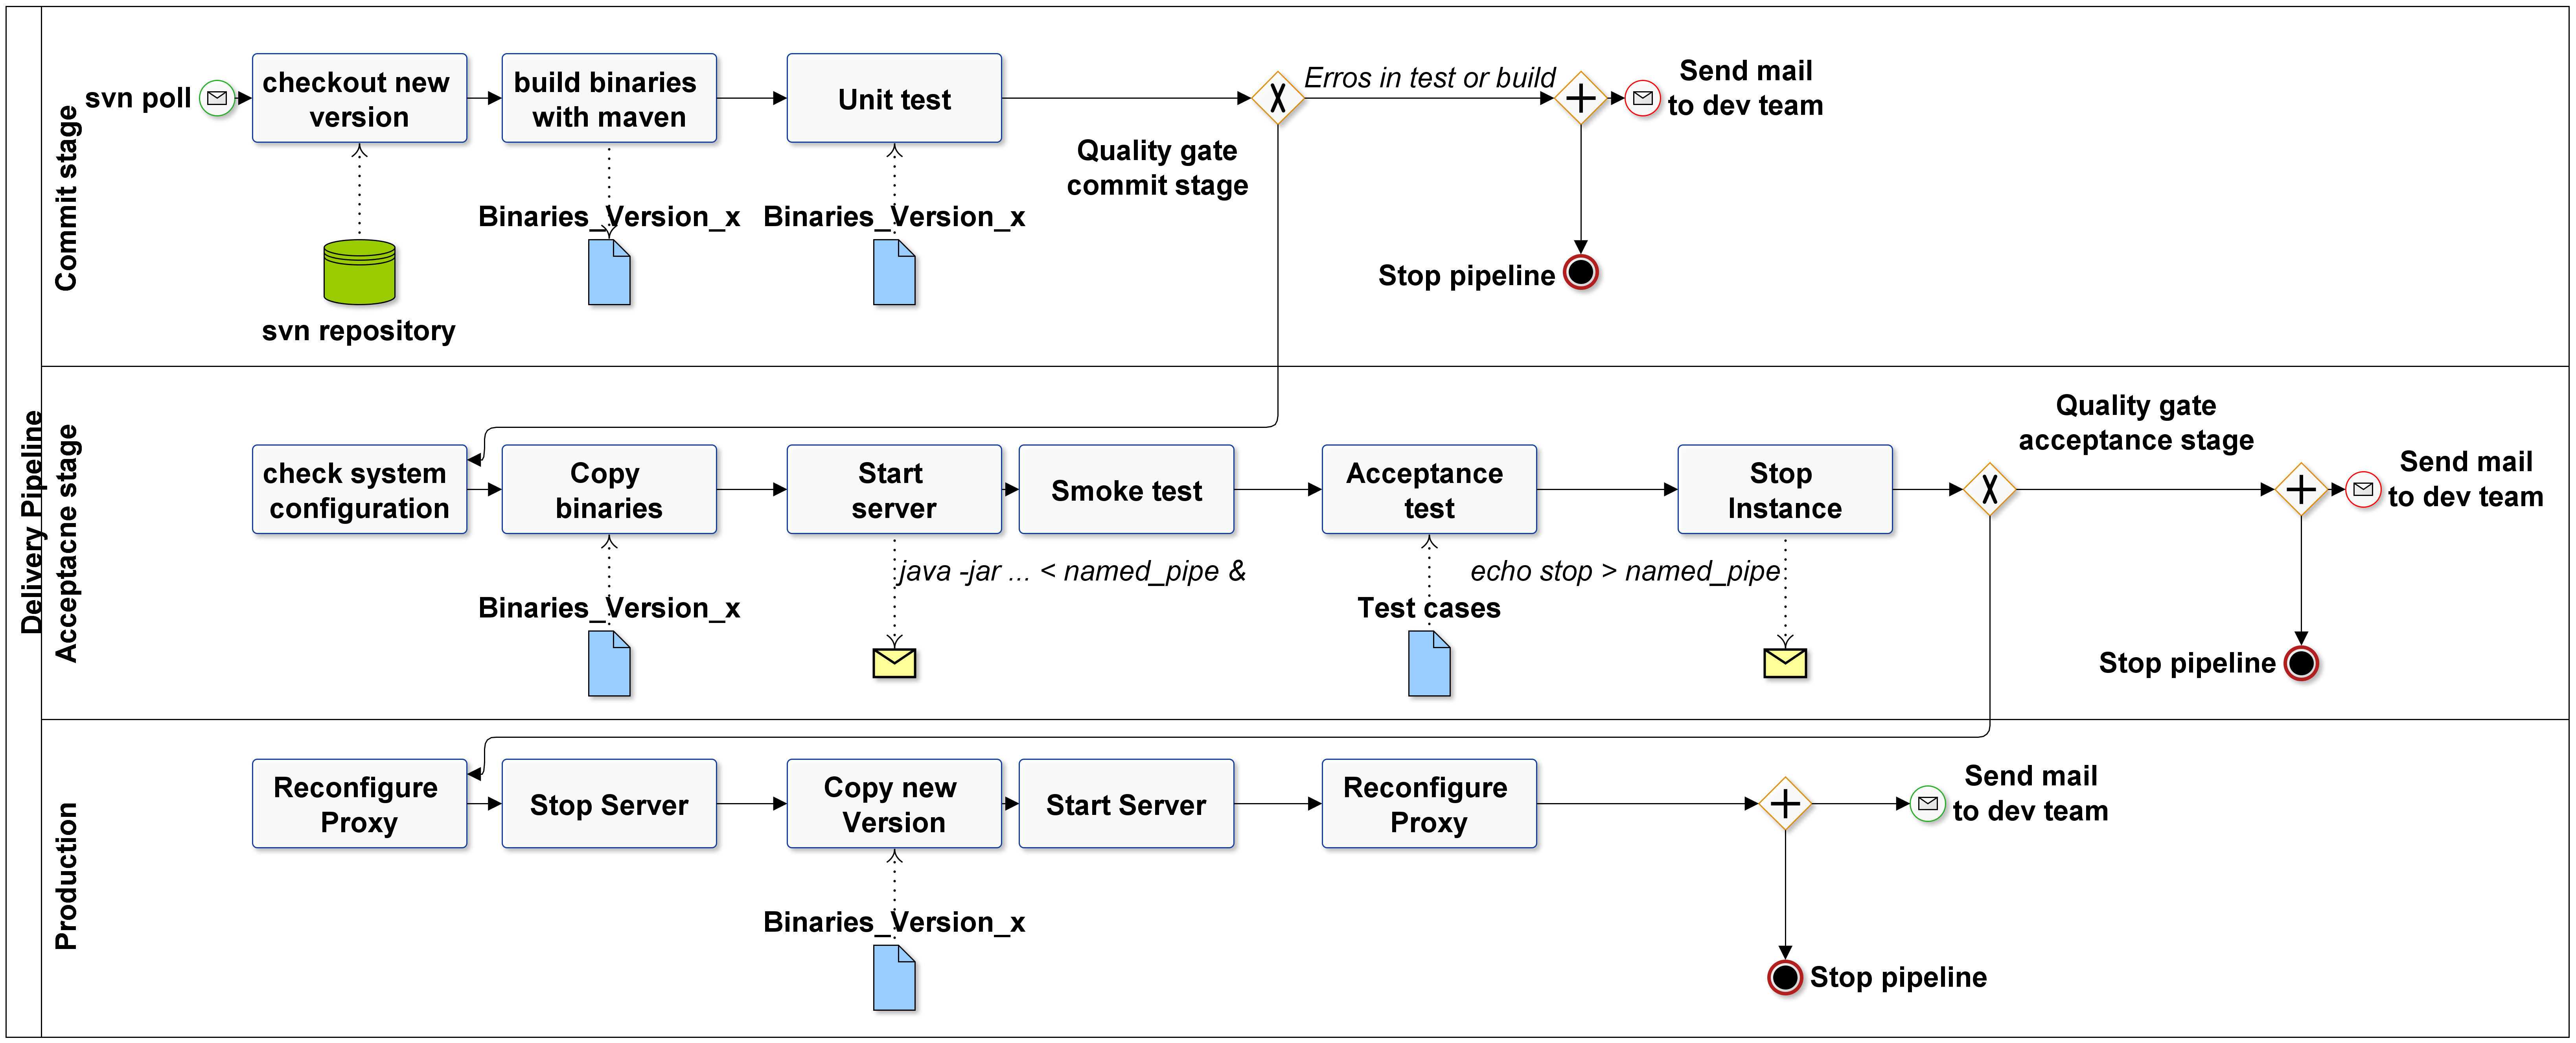
\includegraphics[width=\linewidth]{Grafiken/szenario_1.png}}
\caption{Deployment Pipeline f�r Szenario+1}
\end{figure}

\subsubsection{\comstage}

Ein Entwickler �bermittelt die durchgef�hrten �nderungen am Quellcode der Versionsverwaltung (svn commit). In der Versionsverwaltung wird die Revisionsnummer erh�ht. Die letzte Version, die f�r eine Instanz der Pipeline genutzt wurde, ist \go\ bekannt. Durch eine Abfrage der Versionsverwaltung pr�ft \go\ in einem festen Zeitintervall, ob es �nderungen der Revisionsnummer gibt (svn poll). Ist dem so, wird eine neue Instanz der Pipeline mit der aktuellen Revisionsnummer erzeugt.

Obwohl es in \go\ m�glich ist, in einer Stage Aufgaben durch Jobs zu parallelisieren, gibt es in dieser Pipeline hierf�r keinen Bedarf. Unterhalb der \comstage\ befindet sich deshalb nur ein einziger Job. Ein freier Agent wird mit der Job-Konfiguration initialisiert. Der Agent beginnt mit dem Checkout der aktuellen Quellcode-Basis aus Subversion heraus. Alle Dateien werden im Arbeitsverzeichnis des Agents unter dem Pfad \url{/pipelines/<PIPELINE_NAME>/} abgelegt. Anschlie�end wird Maven �ber den \emph{Custom Command} mit \texttt{mvn install assembly:single} angesto�en. Maven l�dt dabei alle Pakete, von denen die Anwendung abh�ngt, aus dem zentralen Repository, kompiliert den Quellcode, f�hrt die Komponententests durch und pakt alle Abh�ngigkeiten in ein einziges Jar-File zusammen. 

Ein Nachweis der technischen Korrektheit der Version wird dadurch erbracht, dass die Anwendung kompiliert und alle Komponententests durchlaufen. Die \comstage\ beendet erfolgreich und das erste Quality-Gate wurde passiert. 

\subsubsection{\acstage}

Vor der Ausf�hrung der Akzeptanztests wird die Umgebung auf ihre Konfiguration hin untersucht. Jede �nderung der Infrastruktur wird in einem Update-Skript festgehalten. Ein Update-Skript ist durch die Versionsnummern gekennzeichnet, die das System von einer �lteren auf eine neuere Version heben. Folgendes Muster sei als Beispiel gegeben: \texttt{system\_update\_0005\_0006} hebt die Systemumgebung von Version 5 auf 6. Die letzte Versionsnummer wird auf dem System in einer Datei gehalten. Das Update-Skript enth�lt alle �nderungen von einer Infrastruktur-Version auf die n�chste. Die aktuelle Version wird ausgelesen und gepr�ft, ob ein Update-Skript f�r diese Version existiert. Nach der �nderung durch das Skript wird die aktuelle Versionsnummer des Scripts in eine Datei geschrieben, damit sp�tere �nderungen m�glich bleiben.

Da das Testsystem und \go\ sich eine Umgebung teilen, k�nnen das neue Jar-File sowie das Startskript direkt in das Ausf�hrungsverzeichnis kopiert werden. Die Anwendung wird von \go\ gestartet. Hierf�r wird der \emph{Custom Command} genutzt, um das Startscript aufzurufen und ausf�hren zu lassen. Alle Ausgaben der Systemkonsole werden an das Log-File weitergeleitet, dieses kann sp�ter �ber die Oberfl�che von \go\ eingesehen werden.

Nach dem Start wird ein Smoke-Test durchgef�hrt, welcher pr�ft, ob das System grundlegend einsatzbereit ist. Hierf�r wird das Kommandozeilenwerkzeug \emph{curl} genutzt, um ein \emph{GET} der Status-Seite �ber HTTP auszuf�hren. Als Antwort wird ein Response-Status-Code 200 im HTTP-Header erwartet.

Das System ist nun bereit, auf die Erf�llung aller funktionalen und nicht-funktionalen Anforderungen hin untersucht zu werden. Die Testf�lle werden vom Test-Framework geladen und ausgef�hrt. Reagiert das System wie verlangt, kann die \acstage\ abgeschlossen werden.

Die Anwendung �ffnet beim Start einen Eingabekanal auf der Systemkonsole. �ber diesen kann die Anwendung gestoppt und Status-Informationen abgerufen werden. Bei Start des Systems wurde der Eingabekanal auf eine Named-Pipe gelegt und die Anwendung im Hintergrund gestartet. �ber die Named-Pipe kann \go\ der Anwendung nun das Stopp-Kommando geben. Die Anwendung beendet den Server und schlie�t. Anschlie�end wird ausgewertet, ob Fehlermeldungen w�hrend der Tests in das Error-Log geschrieben wurden.

An dieser Stelle kann festgestellt werden, dass die neue Version der Anwendungen auf ihre technische Korrektheit und Erf�llung der Akzeptanzkriterien hin �berpr�ft wurde. Werden bestimmte Akzeptanzkriterien nicht erf�llt, verhindert dies die Auslieferung in die Produktivumgebung. Auch die Auswertung der Fehlerprotokolle spielt hier eine Rolle. Gibt es Eintr�ge im Fehler-Log der Anwendung oder in der Fehlerausgabe auf der Systemkonsole, verhindert dies die Auslieferung. \go\ ist so konfiguriert, dass es dann eine Nachricht an das Entwicklerteam sendet. 

Der Entwickler, der die letzte �nderung vorgenommen hat, ist in der Verantwortung, die Fehlerprotokolle durchzusehen. Zusammen mit dem Projektleiter wird entschieden, ob das Release in die Produktion dennoch stattfinden sollte. Dies geschieht unter Abw�gung aller Risiken.

\subsubsection{\prodenv}

Wenn alle Tests positiv verlaufen sind, wird die Anwendung in die Produktivumgebung ausgerollt. Je nach Art der Umgebung stellt dies einen mehr oder minder komplexen Prozess dar. Das in diesem Szenario genutzte System ist kein kritischer Gesch�ftsprozess mit einer sporadischen Nutzung f�r spezielle Aufgaben. Um einen direkten Systemzugriff zu verhindern, wurde ein Apache HTTP-Server vorgeschaltet, der Anfragen an das System weiterleitet. Der HTTP-Server ist so konfiguriert, dass dieser mit dem Parameter \texttt{-DClosedForNow} neu gestartet wird und anschlie�end Anfragen mit einer Wartungsseite beantwortet. Damit kann das zu aktualisierende System heruntergefahren werden. Der Zugriff auf das Produktivsystem erfolgt �ber  SSH\footnote{SSH: \emph{S}ecure \emph{Sh}ell erm�glicht eine Verbindung zur Kommandozeile entfernter Systeme.}. Ist das System heruntergefahren, wird die neue Version eingespielt. Die alte Version wurde zuvor in das Verzeichnis \texttt{Recover} kopiert, um im Notfall das Recover-Skript starten zu k�nnen und die vorhergehende Version wiederherzustellen.

\section{Szenario 2}

% Web-Anwendung (HTTPD + TOMCAT + SQL)
% jenkins.ci + deployinator.deploy
% langlaufendes Wartungprojekt + DB

% Szenariobeschreibung
% - Wartung und Weiterentwicklung f�r n�chste 2 Jahre, alle 4 Wochen deployment neuer Funktionen + Hot-Fix, wird von adesso gehosted
% - Web-Anwendung
% Aufbau des Projektes
% - JEE + Maven
% - Produktion: Cluster aus 4 Tomcat-Instanzen + HTTPD als Load-Balancer + SQL-DB
% - Test: 1 Tomcat + Test-DB

% Beschreibung der Pipeline
% Jenkins-CI
% - Checkout aus SVN
% - Build mit Maven
% - Komponenten-Tests
% - statische Code-Analyse
% - Repository
% Deployinator.DeployToTest
% - Check Version in Repository
% - Test-Deploy
% 	-> check DB-Update-Skript
%	-> update DB
%	-> Test DB-Health
%	-> Deploy war-file
% 	-> Smoke-Test
% 	-> Run AC-Test ? copy to Good-Rpos : break
% - Ready for manuell Test -> Mail versand
% Deployinator.DeployToProd
% - Check Version in Good_Repos
% - Show something new
% - Deploy
% 	-> check DB-Update-Skript
%	-> Backup DB
% 	-> update DB
% 	-> Test DB-Health
% 	-> Use Sticky Session und Session-sync
% 	-> for (server Server : servers) { server.stop deploy(to.server.home) server.start }
% Deployinator.ProdRollBack

\subsection{Beschreibung und Projektaufbau}

Szenario~2 nimmt ein Kundenprojekt als Ausgangspunkt. Dabei handelt es sich um eine Web-Anwendung f�r Mitarbeiter einer R�ckversicherung, die diese nutzen, um Risikokalkulationen durchf�hren zu k�nnen. Das System befindet sich in einer kontinuierlichen, wenn auch nicht ununterbrochenen, Weiterentwicklung. \cd\ und eine \dpipe\ sollen den Lieferprozess erheblich verk�rzen und den Nutzern alle zwei Wochen neu entwickelte Funktionalit�ten bereitstellen k�nnen. Zudem sollen kurzfristige Fehlerbeseitigungen (Hot-Fix) in die Produktivumgebung eingespielt werden k�nnen.

Als Ausf�hrungsumgebung der Anwendung wird ein JBoss Application Server verwendet sowie das JSF 2.0 Framework eingesetzt. Die Testumgebung besteht aus einer einzelnen Serverinstanz mit angegliederter Testdatenbank. Bei der Produktivumgebung werden vier Instanzen zu einem Cluster verbunden und HTTP-Server als Load-Balancer vorgeschaltet.

Die bestehenden Ma�nahmen der Qualit�tssicherung sind schon als automatisierte Komponenten und Akzeptanztests realisiert worden. Der Build-Prozess wird auf dem CI-System von adesso, dem Jenkins CI-Server, durchgef�hrt. Jede �nderung der Quellcode-Basis in der Versionsverwaltung (SVN) f�hrt zum Ansto�en des Build-Prozesses und zur Ausf�hrung der Komponententests. Akzeptanztests, die in automatisierter Form vorliegen, wurden bisher manuell angesto�en und gegen das Testsystem ausgef�hrt. Auf dem Testsystem existiert ein Hilfsskript. Dieses stoppt den Web-Server, kopiert das neue WAR-File vom Arbeitsverzeichnis des Nutzers in das des Servers und startet dieses neu. Voraussetzung ist das Laden der aktuellen Version aus dem unternehmensinternen Repository. Dieser Schritt wurde so weit automatisiert, als das ein anderes Skript nur noch mit der aktuellen Versionsnummer aufgerufen werden muss. Das Laden der aktuellen Version �bernimmt dann jenes Skript. All diese Aufgaben m�ssen aber manuell aufgerufen werden und ben�tigen die Administrationsrechte f�r den Testserver. Dies gilt analog auch f�r das Produktivsystem.

Ein Teil der \dpipe\ wird bereits durch das CI-System umgesetzt. Build-Prozess und Test der Komponenten k�nnen dort verbleiben. Mit \dpl\ wurde ein Werkzeug evaluiert, welches die bestehenden Ans�tze aufgreifen und miteinander verbinden kann. \dpl\ soll hier genutzt werden, um auf Test- und Produktivumgebung zu deployen und die Erf�llung der funktionalen und nicht-funktionalen Anforderungen zu pr�fen.

\subsection{Aufbau der \dpipe}

Da die \comstage\ schon durch das bestehende CI-System abgebildet wird, werden hier nur \acstage\ und \prodenv\ n�her beschrieben. Bei jedem Durchlauf des CI-Systems werden die erstellten Softwarepakete in einem Repository abgelegt.

\dpl\ als \ssp\ stellt dem Team die M�glichkeit bereit, die aktuelle Version der Anwendung, deren technische Korrektheit mittels Komponententests untersucht wurde, in die Testumgebung zu deployen. Die automatisierten Akzeptanztests k�nnen anschlie�end durchlaufen werden. Nach dem eine Version erfolgreich getestet wurde, kann das Deployment in die Produktivumgebung, am Tag des Release, von einem Mitglied des Entwicklungsteams �ber die Oberfl�che von \dpl\ angesto�en werden.

\dpl\ wurde, wie in Abschnitt~\ref{chap_dpl} beschrieben, um die M�glichkeit erweitert, eine spezifische Version f�r das Deployment ausw�hlen zu k�nnen.

\subsubsection{\acstage}

Ein Mitglied des Entwicklungsteams ruft die Oberfl�che von \dpl\ auf. \dpl\ ermittelt dabei die im Repository abgelegten Versionen und stellt diese in der Auswahlliste bereit. Soll nicht die zuletzt erstellte Version deployt werden, kann eine andere im Drop-Down-Men� ausgew�hlt werden. Mit dem Button \emph{Deploy to test} wird der Deployment-Prozess angesto�en. An der Infrastruktur werden w�hrend der Entwicklung keine �nderungen erwartet, sodass dieser Schritt im automatisierten Deployment nicht weiter ber�cksichtigt wird. Da die Anwendung mit einer Datenbank zusammenarbeitet und hier, im Gegensatz zur Infrastruktur, �nderungen zu erwarten sind, muss der Deployment-Prozess dieses ber�cksichtigen k�nnen. Alle Schritte, die w�hrend des Deployments durchgef�hrt werden, sind im Stack-Modul von \dpl\ definiert. Dabei werden die hinterlegten Skripte auf der Systemkonsole �ber \lstinline$run_cmd$ aufgerufen.

Der erste Schritt des Deployments ist die Aktualisierung der Deployment-Skripte, welche in der Versionsverwaltung von Subversion in der aktuellen Version hinterlegt sind. Die �nderungen an der Datenbank werden durch ein Update-Skript organisiert. Auch diese werden in der Versionsverwaltung gehalten und gepflegt. 

Update und Rollback der Datenbank werden inkrementell durchgef�hrt. Die Datenbank speichert hierf�r die aktuelle Versionsnummer. Ist die Datenbank von einer Version auf die n�chste anzuheben, wird ein Update-Skript erstellt, welches die notwendigen Anweisungen enth�lt. Auch der inverse Vorgang, ein Rollback, muss ber�cksichtigt werden. Auch hierf�r muss ein Skript existieren, welches die inversen Operationen des Update-Skriptes enth�lt. Soll eine Softwareversion deployt werden, wird gepr�ft, welche Version der Datenbank f�r die Version der Anwendung ben�tigt wird. Diese Information kann dem Softwarepaket selbst �ber die Datei \texttt{db.info} durch den Parameter \texttt{db\_version} entnommen werden. F�r das Datenbankupdate existiert ein Skript, welches die Notwendigkeit einer Ver�nderung pr�ft und diese dann ausf�hrt.

Verlangt die neue Version \zb\ Version $6$ der Datenbank, diese aber den Stand der Version $4$ hat, muss zuerst das Skript \texttt{db\_update\_4\_5.sql} ausgef�hrt werden, um anschlie�end das Update \texttt{db\_update\_5\_6.sql} ausf�hren zu k�nnen. Wird ein Rollback notwendig, so ist \zb\ zuerst das Skript \texttt{db\_rollback\_6\_5.sql} und dann das Skript \texttt{db\_rollback\_5\_4.sql} ausgef�hrt werden.

Bevor die Datenbank aktualisiert werden kann, ist zu pr�fen, ob die Instanz des Testservers aktiv ist. In diesem Fall wird der Server heruntergefahren. Anschlie�end wird eine Sicherung der Datenbank durchgef�hrt. Nach dem Update ist eine �berpr�fung des Zustandes der Datenbank notwendig. Der Health-Check und die Sicherung sind Teil des Skriptes.

Nachdem die �berpr�fung des Zustandes der Datenbank den erfolgreichen Verlauf des Updates best�tigt hat, kann die Software auf dem Testserver aktualisiert werden. Der Server wird wieder hochgefahren. Alle Befehle werden hierzu �ber SSH ausgef�hrt. Die Datenbankaktivit�ten k�nnen \zb\ �ber \emph{SQL*Plus}\footnote{Weitere Informationen zu SQL*Plus unter: \url{http://docs.oracle.com/cd/B19306_01/server.102/b14357/toc.htm}} ausgef�hrt werden.

Das Testsystem hat nun den notwendigen Zustand, um die neue Version auf die Einhaltung der Anforderungen zu �berpr�fen. Die automatisierten Akzeptanztests k�nnen nun durchgef�hrt werden. Die hierf�r genutzten Testframeworks sind auf dem System, auf dem auch \dpl\ ausgef�hrt wird, installiert. Alle Testf�lle sind am Anfang der \acstage\ aus der Versionsverwaltung geladen worden.

Die Testprotokolle, die bei einem Durchlauf der Akzeptanztests entstehen, werden gepackt und f�r eine sp�tere Auswertung in das Repository des Servers kopiert. Das Testteam erh�lt die Testprotokolle ferner als Anhang der E-Mail-Nachricht, die zum Abschluss der Phase versandt wird.

Sofern im Testprozess Fehler auftreten, kann dies erfasst und darauf reagiert werden. Laufen alle Tests fehlerfrei durch, wird die Versionsnummer des gepr�ften Softwarepaketes in einer Liste mit erfolgreich getesteten Versionen eingetragen.

\subsubsection{\prodenv}

Die Schritte beim Deployment in die Produktivumgebung verlaufen �hnlich wie beim Deployment in die Testumgebung. Gleich sind das Laden der Skripte aus der Versionsverwaltung und das Update der Datenbank. 

W�hrend des Aktualisierungsvorgangs steht die Anwendung nicht zur Verf�gung. Der Proxy-Server leitet alle Anfragen f�r den Zeitraum der Aktualisierung auf eine Wartungsseite. Dieses l�uft dabei genauso ab, wie in Szenario~1 schon beschrieben.

Nachdem der Proxy konfiguriert wurde, k�nnen die Web-Server angehalten werden, damit das Datenbankupdate eingespielt werden kann. Ist dies erfolgreich verlaufen, werden die Web-Server aktualisiert und neu gestartet. Der Proxy-Server wird dann wieder normal konfiguriert.

Da die Anwendung nicht bei jeder �nderung, sondern nur alle zwei Wochen, in die Produktivumgebung ausliefert, ist der Deployment-Prozess weniger komplex gestaltet. Dies sollte \zb\ f�r eine Anwendung, die einem stetigen Zugriff unterliegt, nicht der Fall sein. Das gleichzeitige Herunterfahren aller Produktivinstanzen w�re dann keine Option. Das System von Szenario~2 wird aber nicht mehr am Freitag nach 17~Uhr verwendet, sodass der Aktualisierungsvorgang danach auch mit geringerer Komplexit�t durchgef�hrt werden kann.

Alternativ k�nnte dies in anderen Anwendungssituationen so gestaltet sein, dass die Datenbank vor einem Update auf ein Zweitsystem gespiegelt wird. Alle �nderungen w�rden dann auf dem Zweitsystem ausgef�hrt. Das Update der Anwendung wird dann inkrementell auf allen Servern durchgef�hrt. Die neue Anwendung arbeitet mit der neuen Datenbankversion, der alte Softwarestand mit der alten Version der Datenbank. Nach dem alle Server aktualisiert worden sind, m�ssen die �nderungen, die in der Zeitspanne des Updates durchgef�hrt worden sind, auf die neue Datenbank �bertragen werden. Eine weitere Voraussetzung ist der Austausch von Informationen aktiver Nutzer-Sessions zwischen den Servern, damit ein Herunterfahren einer Instanz nicht zu einem Informationsverlust f�hrt.

\section{Zusammenfassung}

Grundlage der hier beschriebenen Szenarien waren Projekte, mit denen der Verfasser der Arbeit w�hrend seiner T�tigkeit im Unternehmen in Ber�hrung gekommen war. Die Szenarien wurden so angepasst, dass diese als Ausgangspunkt f�r eine m�gliche Umsetzung von \cd\ durch die untersuchten Werkzeuge aufzuzeigen konnten.

Beide Szenarien stellen M�glichkeiten der Verwendbarkeit der untersuchten Werkzeuge dar und sind noch keine optimalen L�sungen. Diese k�nnen nur durch das Zusammenwirken von IT-Betrieb, Entwicklungsteam und Kundenvertretern gemeinsam erarbeitet werden.

Die Umsetzung einer \dpipe\ ist mit \go\ einfacher, da Quality-Gates einfacher in den Prozess einzurichten sind. Kann das CI-System aus bestimmten Gr�nden nicht genutzt werden, bietet sich \go\ als eine Alternative an, alle Elemente von \cd\ in einer Umgebung konfigurieren und steuern zu k�nnen. \dpl\ hingegen erg�nzt das CI-System. Die Umsetzung einer \acstage\ ist jedoch nicht sehr komfortabel. In \dpl\ k�nnen keine Testprotokolle angezeigt werden. Das System muss um eine Liste gepr�fter Versionen erg�nzt werden, um ermitteln zu k�nnen, welche Version aus dem Repository  die notwendige Reife besitzt, um in die Produktivumgebung ausgeliefert werden zu k�nnen.

% Fazit3w

\chapter{Fazit}

Im Rahmen dieser Arbeit sollte sich allgemein mit dem Themenkomplex des \cd\ auseinandergesetzt werden. Speziell standen in diesem Zusammenhang drei als interessant eingestufte Werkzeuge im Fokus, die n�her untersucht werden sollten. Im Vorfeld der Untersuchung wurde auf die Beziehung zwischen \cd\ und \devops\ eingegangen. Anschlie�end wurden die Konzepte von \cd , wie sie \hf\ vorschlagen, beleuchtet. Dies war einf�hrend notwendig, um f�r adesso der Frage nach der Funktionsweise sowie dem jeweilig verfolgten Ansatz der zu untersuchenden Werkzeuge nachgehen zu k�nnen. Zudem sollte nach m�glichen Synergien f�r den derzeitigen Lieferprozess gesucht werden.

\section{Erkenntnisse}

Mit einem Fragebogen an das unternehmenseigene CI-Team wurden die etablierten Lieferstrukturen ermittelt. Eine Erkenntnis f�r die Umsetzungsm�glichkeiten von \cd , welche aus dem Fragebogen abgeleitet werden konnte, war die der ungleichen Projektstruktur bei adesso. Diese kommt durch die individuelle Softwareentwicklung und deren starke Ausrichtung an das Projektgesch�ft zustande. Dabei wird f�r adesso die Umsetzung eines allgemeing�ltigen Lieferprozesses verhindert, welcher von allen Projekten auf gleiche Weise genutzt werden kann. Vielmehr sind projektspezifische Faktoren bei der Einrichtung des Lieferprozesses heranzuziehen, die von Projekt zu Projekt variieren k�nnen. adesso unterst�tzt die Projektteams durch einen zentralen Build-Prozess bei der Realisierung von \ci . Dies stellt eine zentrale Voraussetzung f�r die Umsetzung von \cd\ dar.

Im Verlauf der Arbeit zeigte sich, das \cd\ nicht durch eine bestimmte Technologie oder ein einzelnes Werkzeug l�sbar ist. Es entstand die Annahme, dass die zu untersuchenden Werkzeuge nur die L�sung eines Teilproblems von \cd\ erm�glichen k�nnen. Diese Annahme best�tigte sich bei der Evaluierung. Das Kernproblem von \cd , ein automatisiertes Deployment in verschiedene Umgebungen zu erm�glichen, l�sen die Werkzeuge nicht, erm�glichen es aber, die Implementierung eins Lieferprozesses in Bezug auf \go\ zu organisieren bzw., in Bezug auf \dr\ und \dpl , ansto�en zu k�nnen.

Zum Ende der Arbeit trat die Erkenntnis hervor, dass \go , \dr\ und \dpl\ 
\cd\ durch die beschriebenen Ans�tze unterst�tzen, diese aber nicht direkt als Werkzeuge f�r \cd\ angesehen werden k�nnen, da sie nur eine Kategorie von notwendigen Funktionen und Eigenschaften f�r die Realisierung von \cd\ abdecken. \cd\ kann nur aus einer intelligenten und auf den Bedingungen der zu liefernden Software abgestimmten Kombination verschiedener Werkzeuge und Skripte m�glich werden. \emph{Das} Werkzeug f�r \cd\ kann nicht erwartet werden.

Den Lieferprozess auf einfache Weise starten zu k�nnen ist ein wichtiger Baustein im automatisierten Lieferprozess, hilft aber nicht bei der L�sung der kritischen Fragen von \cd . Dies sind \zb\ die sichere und verlustfreie Aktualisierung der Datenbank einer Web-Anwendung bei laufendem Betrieb oder das inkrementelle automatische Update einer Web-Anwendung, ohne das dies eine Auswirkung auf die aktiven Nutzer hat.

Vielmehr unterst�tzen die untersuchten Werkzeuge die Verwirklichung von \devops\ durch die M�glichkeit, eine aus Skripten und Werkzeugketten bestehende automatisierte \dpipe\ ansto�en zu k�nnen. IT-Betrieb und Entwicklerteam r�cken n�her zusammen, sodass der zu realisierende Deployment-Prozess nur in einer engen Zusammenarbeit m�glich wird.

\go\ bietet hier als Teill�sung f�r \cd\ die am weitesten gehende Implementierung einer Steuerung des Lieferprozesses an. Basierend auf Tasks, Jobs und Stages sowie der einfachen Umsetzung von Quality-Gates k�nnen alle Prozesse der \dpipe\ in \go\ organisiert werden. \dr\ und \dpl\ sind als reine Push-Button-L�sungen einfacher aufgebaut, k�nnen aber an bestehende Prozesse des CI-Systems angekoppelt werden.

In der Kombination der Erkenntnisse des Fragebogens und der Untersuchung der Werkzeuge, wurden zwei m�gliche Szenarien vorgestellt, wie diese L�sungen in zuk�nftigen Projekten zum Tragen kommen k�nnten. F�r Projekte, die nicht auf die interne CI-Infrastruktur von adesso zur�ckgreifen k�nnen, ist \go\ ein gutes und schnell verf�gbares Werkzeug, um \ci\ und ein \dpipe\ realisieren zu k�nnen. F�r Projekte, die das CI-System bereits nutzen, automatisierte Akzeptanztests implementiert haben und mit Deployment-Skripten die Umgebung konfigurieren und ausliefern, ist \dpl\ das richtige Werkzeug, diese Elemente verbinden zu k�nnen.

\section{Ausblick und Ankn�pfungspunkte}

Auf die dringenden Fragestellungen von \cd , verschiedene Systeme bei laufendem Betrieb aktualisieren zu k�nnen, konnte in dieser Arbeit nicht eingegangen werden. Es blieb bei der Betrachtung von Werkzeugen f�r die Prozessteuerung bzw. f�r die Aktivierung schon hinterlegter automatisierter Auslieferungsprozesse.

In diesem Zusammenhang ergeben sich weitere interessante Ankn�pfungspunkte f�r die Realisierung von \cd :

% Erprobung der beiden Versionen in echten Projekten
% automatisierte Konfiguration mit Chef
% Provisionierung von IaaS f�r Systeme


\begin{itemize}
\item Die Erprobung von \dpl\ und \go\ in einem realen Projektumfeld. F�r eine Vergleichbarkeit der Ans�tze sollte dies an einem zu bestehenden Projekt umgesetzt werden k�nnen. Dieses sollte dann schon feste Abl�ufe des Lieferprozesses definiert haben. Daraus k�nnten weitere Schlussfolgerungen gezogen werden, wie sich die so implementierte \dpipe\ auf Produktivit�t des Entwicklungs- und Testteam auswirken kann. Zudem sind in einem realen Projektumfeld auch die Bedingungen des Produktivsystems bekannt, die in den beschriebenen Szenarien nur angerissen werden konnten.
\item Die Erarbeitung von Ans�tzen, \dpl\ und \go\ mit Werkzeugen wie Chef zu verbinden, um Infrastrukturen automatisch zu konfigurieren. Dieser Punkt konnte in dieser Arbeit nur in einer groben und abstrakten Form angerissen werden. Es sollten hier aber die St�rken und Schw�chen einer solchen Verbindung noch n�her beleuchtet werden. \cd\ besitzt an dieser Stelle m�glicherweise noch Schwachstellen, die eine \dpipe\ bzw. die mit ihr verbundenen Systeme instabil werden l�sst. Dies sollte noch n�her untersucht werden.
\item Eine m�gliche Verbesserung k�nnte auch das Ausnutzen von Infrastructure-As-A-Service in Verbindung mit einer Umsetzung von Private- bzw. Hybrid-Cloud im Unternehmen bedeuten. Hier wurden schon in Form einer Master-Thesis von Marko Salchow eine entsprechende Beschreibung geliefert, wie der Aufbau einer Hybrid-Cloud mit OpenStack\footnote{Weitere Informationen zu OpenStack unter \url{http://www.openstack.org/}} und unter Zunahme einer Cloud-API realisiert werden k�nnte. Salchow kam zum Schluss dass die Nutzung von Abstraktions-APIs gewinnbringend sein kann, obwohl in einem komplexen Szenario eine Umsetzung mit OpenStack nur durch einen erh�hten Aufwand verwirklicht werden kann.\footnote{Vgl. \cite{Salchow2012}} Von seiner Arbeit ausgehend, k�nnten aber vertiefende Szenarien in Zusammenhang mit \cd\ entwickelt werden. An deren Ende k�nnte die Realisierung einer \dpipe\ mit der automatischen Versorgung von Rechnerinstanzen in einer Private-Cloud stehen. Ben�tigte Instanzen f�r die Testdurchf�hrung k�nnten so auf einfache Weise erzeugt und der \dpipe\ zur Verf�gung gestellt werden.
\item Ein automatisierter Auslieferungsprozess, der direkt in die Produktivumgebung eines Kunden liefert, muss alle funktionalen und nicht-funktionalen Anforderungen erf�llen k�nnen. Der Ansatz von BDD liefert hier einen geeigneten Beitrag, Akzeptanztests schon zu Beginn in die \dpipe\ fest zu implementieren. BDD hat adesso parallel zu \cd\ in Form einer Master-Thesis evaluieren lassen. Robert Weber kam in seiner Arbeit zur Ansicht, dass BDD zwar einen erh�hten Implementierungsaufwand erfordert, dies aber in Verbindung mit \cd\ relativiert wird. Der Gesamtaufwand, der durch die erh�hte H�ufigkeit des kontinuierlichen Lieferprozesses entsteht, kann durch automatisierte Durchf�hrung von Akzeptanztests deutlich reduziert werden. \footnote{Vgl. \cite{Weber2012}} Dieses sollte bei zuk�nftigen Projekten Ber�cksichtigung finden.
\item Bei einem automatisierten Auslieferungsverfahren ergibt sich eine weitere Komplexit�t durch die Aktualisierung des Produktivsystems im laufenden Betrieb, wenn \zb\ das Datenbank-Schema aktualisiert werden soll. Ein Datenbank-Update wird in Verbindung mit dokumentenbasierten Datenbanken aber vereinfacht. Zum Thema \emph{Big Data und NoSQL} bietet Robert Zeschkes 2012 verfasste Master-Thesis bei adesso einen Ankn�pfungspunkt, der in Verbindung mit \cd\ noch n�her betrachtet werden sollte. Da bei einer dokumentenbasierten Datenbank keine Verwerfungen auftreten, wenn Objekte mit neuen Attributen gespeichert werden, sind diese Systeme durchaus f�r eine Verwendung im kontinuierlichen Lieferprozess geeignet.\footnote{Vgl. \cite{Zeschke2012}}
\end{itemize}

% Aktualisierung einer laufenden Anwendung
% Aktualisierung einer DB bei laufenden Betrieb

Die Themen \cd und \devops , IaaS in einer Hybried-Cloud, BDD und Big Data und NoSQL verbindet adesso unter den Namen \emph{New Shool of IT}. adesso h�lt hier eine neue strategische Ausrichtung der IT-Branche mit anderen Dienstleistungen und Angeboten f�r m�glich.\footnote{Vgl. \cite{Wolff2012}}

% adesso und strategische ausrichtung


\chapter*{Eidesstattliche Erkl�rung}
%\addcontentsline{toc}{chapter}{Eidesstattliche Erkl�rung} 

Ich versichere, die von mir vorgelegte Arbeit selbstst�ndig verfasst zu haben. Alle Stellen, die w�rtlich oder sinngem�� aus ver�ffentlichten oder nicht ver�ffentlichten Arbeiten anderer entnommen sind, habe ich als entnommen kenntlich gemacht. S�mtliche Quellen und Hilfsmittel sind angegeben. Die Arbeit hat mit gleichen bzw. in wesentlichen Teilen gleichem Inhalt noch keiner Pr�fungsbeh�rde vorgelegen.\\\bigskip

Stralsund, den \today \\\vspace{3cm}

Andr� G�rtner

%\TODO{noch einzuf�gen!}

\bibliographystyle{alphadin}
\bibliography{bibliographie}

\renewcommand{\thepage}{}

\part{Anh�nge}

\renewcommand{\thepage}{A-\arabic{page}}
\setcounter{page}{1}
\setcounter{chapter}{0}

\newcommand{\qst}[1]{\noindent\begin{minipage}{\linewidth}\vspace{\baselineskip}\hrule\vspace{5pt}\textbf{\textit{\textsf{#1}}}\end{minipage}}

\newcommand{\answt}[1]{\vspace{\baselineskip}\noindent\textbf{\textsf{#1}}}

\newcolumntype{L}{>{\raggedright\arraybackslash}X}

\renewcommand{\arraystretch}{1.4}

\newcommand{\Antwort}{\answt{Antwort: }}

\newcommand{\Anmerkung}{\answt{Anmerkung: }}

\newcommand{\Zustimmung}{\answt{Zustimmung: }}

%
% Dokument
%

\chapter{Zusammenfassung Fragebogen CI-Team}\label{anhang_entwicklungsstand}

\section{Skizze / Phasen des derzeitigen Entwicklungs- und Auslieferungsprozesses}

\qst{Bitte skizzieren Sie den derzeitigen und Prozess der Softwareerstellung von der Erstellung bis zur Auslieferung.}

\urldef{\adessowiki}{\url}{https://www.adesso.de/wiki/index.php/Continuous_Integration#Build-Pipeline}
\answt{Antwort:} \emph{Verweis auf das Unternehmens-Wiki von adesso. Hierunter fallen demnach die Phasen Build, Smoke-Test, Integrationstest, Regressionstest und Web-Test}\footnote{Vgl. \adessowiki}

\Antwort
\begin{itemize}
\item Setup Entwicklungsumgebung
\item Entwicklung, Subphasen: Checkin $->$ Build \& Unittests $->$ Automatisierte Deployments $->$ Automatisierte (Integrations-)Tests
\item Integrationstests
\item Delivery
\end{itemize}

\Antwort
\begin{enumerate}
\item Entwicklung, meist TDD
\item Build
\item Unit-Tests
\item Integrations Tests
\item ggf. Deploy auf Testsystem / Staging System
\item ggf manuelles Testen oder exploratives Testen
\item Release bzw. Auslieferung manuell, wenn 1-7 ok
\end{enumerate}

\qst{Welche Phasen, von der Erstellung bis zur Auslieferung von Software, werden unterschieden?}

\Zustimmung

\noindent\begin{tabularx}{\textwidth}{Lrr}
Kompilierung des Quellcode & 2 & 67\% \\
Unit- und Komponententests / Analye & 2 & 67\% \\
automatisierte Akzeptanztests & 1 & 33\% \\
automatisierte Kapazit�tstests & 2 & 67\% \\
manuelle Testsstage & 1 & 33\% \\
Konfigurieren von Test- und Produktivumgebung & 1 & 33\% \\
Installation und der Release der Software & 2 & 67\%
\end{tabularx}

\Antwort
Integrations-Tests

\Antwort
diese sind in jedem Projekt ganz individuell!

\section{Commit-Stage}

\qst{Aussagen zur Commit-Stage}

\Zustimmung

\noindent\begin{tabularx}{\textwidth}{Lrr}
Gew�hnlich wird die Software auf einem Entwickler-System gebaut und paketiert. & 0 & 0\% \\
Es gibt einen standardisierten Prozess f�r das Bauen / Paketieren einer Anwendung. & 2 & 67\% \\
Wenn Quellcode kompiliert wurde, wird dieser in allen nachfolgenden Phasen verwendet und nicht noch einmal kompiliert. & 3 & 100\% \\
Erstellte Softwarepakete werden mit einer fortlaufenden Versionsnummer versehen. & 2 & 67\% \\
Alle im Prozess erstellten Softwarepakete werden mit einer fortlaufenden Versionsnummer versehen. & 1 & 33\% \\
Alle Artefakte, die beim Kompilieren und Testen entstehen, werden in einem zentralen Repository aufbewahrt. & 3 & 100\% \\
Dateien und Information zur Konfiguration der erstellten Software werden in einem gesch�tzten Speicher zentral verwaltet. & 2 & 67\% \\
Es werden �bersichtliche Berichte erstellt, die eine qualitative Aussage einer bestimmten Version erm�glichen. & 1 & 33\%
\end{tabularx}


\Anmerkung
auch hier: ist in jedem Projekt ganz individuell!

\qst{Wie werden Softwareentwicklungsprojekte beim Konfigurationsmanagement unterst�tzt?}

\Antwort
Es gibt Vorlagen f�r Ant und Maven

\Antwort
Das Startup (vormals CI) team unterst�tzt durch Beratung und Doing in der Startup-Phase eines Projektes. Weiterhin werden Templates f�r Buildsysteme z.V. gestellt, damit Projekte einheitlich gebaut werden (ANT bereits vorhanden, Maven und Gradle-Templates in Vorbereitung). 

\Antwort
\begin{itemize}
\item Beratung
\item �ber Ticketsystem, um Einrichten von CI Jobs oder bsp. Sonar zu triggern
\end{itemize}

\qst{Wie wird mit Abh�ngigkeiten zu externen Bibliotheken bzw. Komponenten von Drittanbietern umgegangen?}

\Antwort
�ber einen eigenen Nexus-Server

\Antwort
3rd-Party Bibliotheken werden auf einem zentralen Nexus in einem daf�r vorgesehenen Repository abgelegt. Die Projekte sind verantwortlich f�r die Einhaltung der Compliance, z.B. d�rfen Libs, deren Lizenz eine Auslieferung verhindern (z.B. SUN JDK Bibliotheken, JDBC-Treiber usw.) nicht mit ausgeliefert werden.

\Antwort
Nexus als Repository Manager und Proxy zu anderen Repositories

\qst{Wie wird der Build-/ Test-Prozess ausgel�st?}

\Zustimmung

\noindent\begin{tabularx}{\textwidth}{Lrr}
Kompilierung, Paketierung und Test werden jeweils durch einzelne Kommandos auf der Konsole durchgef�hrt. & 0 & 0\% \\
F�r den Prozess existieren Skripten, die das Bauen, Paketieren und Testen der Anwendung durchf�hren. & 0 & 0\% \\
Wir haben automatisierte Prozesse, die durch Ereignisse, z.B. Entwickler-Commit in der Versionsverwaltung, ausgel�st werden. & 2 & 67\%
\end{tabularx}

\Anmerkung
individuell

\qst{Anmerkung zur Commit-Stage:}

\Anmerkung
Jedes Projekt handhabt dies ganz individuell!

\section{Acceptance-Stage}

\qst{Aussagen zum Testbetrieb:}

\Zustimmung

\noindent\begin{tabularx}{\textwidth}{Lrr}
 & Zustimmung &  Anteil \\
Es gibt vereinzelt ein paar automatisierte Unit- und Komponententests. & 1 & 33\% \\
Bei einer �nderung des Softwarestandes werden der gr��te Teil der Tests wiederholt (Regressionstest). & 3 & 100\% \\
Es wird eine statische Code-Analyse durchgef�hrt. & 2 & 67\% \\
Funktionalen Anforderungen werden automatisiert getestet. & 2 & 67\% \\
Unit- und Komponententest werden mit einer hohen Abdeckung durchgef�hrt. & 3 & 100\% \\
Wenn manuelle Tests durchgef�hrt werden, basieren diese auf speziellen Risikoszenarien. & 1 & 33\% \\
Die Anwendung wird nach bestimmten Sicherheitsaspekten analysiert. & 1 & 33\% \\
Es wird auf eine Testabdeckung von 100\% Wert gelegt. & 0 & 0\% \\
Test- und Produktivumgebung sind zu gro�en Teilen identisch. & 1 & 33\% \\
Testberichte k�nnen von allen Projektbeteiligten eingesehen werden. & 1 & 33\%
\end{tabularx}

\qst{Welche Werkzeuge und Methoden werden zur statischen Analyse des Quellcodes angeboten?}

\Antwort
Sonar und FindBugs

\Antwort
Sonar (kapselt Findbugs, Jococo, Checkstyle, PMD, Cobertura)

\Antwort
Sonar, Findbugs, PMD

\qst{Welche Werkzeuge werden zur Aufdeckung von m�glichen Sicherheitsl�chern verwendet bzw. angeboten?}

\Antwort
s. oben (Findbugs hat einige Security-Regeln)

\qst{Welche Werkzeuge nutzen Sie f�r automatisierte Akzeptanz- und Kapazit�tstests?}

\Antwort
JMeter, Selenium

\Antwort
JUnit, JBehave

\qst{Welche Informationen k�nnen aus den Testberichten entnommen werden?}

\Antwort
Alle wesentlichen ;-) Abdeckung Erfolg, Nichterfolg 

\Antwort
Fehlerhafte Tests, Testabdeckung

\qst{Nach welchen architektonischen Vorgaben / Br�chen wird die erstellte Software hin untersucht?}

\Antwort
Modularit�t, Complexit�t, Koh�sion

\qst{Gibt es bestimmte Strategien f�r den Umgang mit Testdaten?}

\Antwort
teilweise

\qst{Anmerkungen zur Acceptance-Stage}

\Anmerkung
Auch hier: in jedem Projekt ganz individuell

\section{Deployment}

\qst{Welche Verfahren werden genutzt, um eine releasef�hige Software in die Produktivumgebung auszuliefern?}

\Antwort
Releases werden �ber Jenkins ausgeliefert

\Antwort
manuelles Delivery $\rightarrow$ es ist mir nicht bekannt, dass wir in eine Prod-Umgebung eines Kunden automatisiert zugreifen und deployen k�nnten. Zudem steht einem automatisierten Deployment in vielen Unternehmen die SOX-Compliance entgegen, die besagt, dass Entwicklung und Produktion strikt zu trennen ist.

\Antwort
Skripte (Shell, Ant), Manuell

\qst{Wie wird das Software-Deployment durchgef�hrt?}

\Zustimmung

\noindent\begin{tabularx}{\textwidth}{Lrr}
 & Zustimmung &  Anteil \\
Es gibt derzeit keine Deployment-Skripte. & 0 & 0\% \\
Deployment-Skripte werden vorwiegend �ber die Konsole angesto�en. & 1 & 33\% \\
Deployment-Skripte werden automatisch angesto�en, sofern ein bestimmtes Quality-Gate durchschritten wurde. & 0 & 0\% \\
Es gibt eine Oberfl�che von der aus das Deployment einer bestimmten Version angesto�en werden kann. & 1 & 33\%
\end{tabularx}

\Anmerkung
individuell, meist �ber Ant oder Maven

\qst{Werden Projektteams bei der Erstellung eines Deployment-Skriptes unterst�tzt?}

\Zustimmung

\noindent\begin{tabularx}{\textwidth}{Lrr}
 & Zustimmung &  Anteil \\
Es gibt keine Unterst�tzung, da die Projekte dies selbst regeln. & 0 & 0\% \\
Es gibt ein paar Skripte aus anderen Projekten, die als Vorlage genutzt werden k�nnen. & 1 & 33\% \\
Es gibt Templates f�r unsere Standardwerkzeuge. & 1 & 33\% \\
Es gibt Tools, mit denen sich das Deployment konfigurieren l�sst. & 1 & 33\%
\end{tabularx}

\qst{Welche Werkzeuge werden f�r das Deployment genutzt?}

\Antwort
ant und Shell-Skripte

\Antwort
Ant mit Shellscripten f�r App-Server, die keine dedizierte Schnittstelle oder Plugin f�r Ant/Maven bieten. Falls diese Ant-Tasks oder Maven-Plugins anbieten (z.B. Apache Tomcat) werden diese genutzt

\qst{Wie wird mit Konfiguration von Test- / Produktivumgebungen umgegangen?}

\Zustimmung

\noindent\begin{tabularx}{\textwidth}{Lrr}
 & Zustimmung &  Anteil \\
Abh�ngige Komponenten werden vor dem Betrieb bzw. Test manuell installiert. & 1 & 33\% \\
Projekte erstellen eigene Skripte, um die ben�tigten Komponenten zu installieren. & 2 & 67\% \\
Es gibt Template-Skripte, um Standardumgebungen zu installieren und zu konfigurieren. & 0 & 0\%
\end{tabularx}

\qst{Existieren derzeit Bem�hungen eine Delivery-Pipeline in einzelnen Softwareentwicklungsprojekten umzusetzen?}

\Zustimmung

\noindent\begin{tabularx}{\textwidth}{Lrr}
 & Zustimmung &  Anteil \\
Es gibt noch kein Einsatzszenario bzw. Interesse. & 0 & 0\% \\
Es sind Projekte in Zukunft geplant. & 0 & 0\% \\
Es gab / gibt schon Pilotprojekte. & 1& 33\% \\
Eine Delivery-Pipeline haben wir schon �fter umgesetzt. & 1 & 33\%
\end{tabularx}

\qst{Anmerkungen zum Deployment}

\Anmerkung
Auch hier: alles individuell, insbesondere was die Produktivsetzung angeht. Zur Frage \emph{Wie wird mit Konfiguration von Test- / Produktivumgebungen umgegangen?} Auch hier ganz unterschiedlich, aber meist manuell. Bei der AMS haben wir nun in einer Cloud-Umgebung Chef im Einsatz um Server automatisiert zu provisionieren.

\end{document}